% P1 ACADEMIC-WRITING PREVIEW (2026-11-24) of the CellCharter research unit.
% Builds on REV_P0 (kept unchanged); V1 and layout V2 also unchanged. NOT compiled in the
% assistant session (no TeX on that machine). Not the full dissertation; must later be moved into
% the school's official thesis template. Compile: xelatex -> bibtex -> xelatex -> xelatex.
\documentclass[UTF8,a4paper,12pt]{ctexart}
\usepackage[margin=2.4cm]{geometry}
\usepackage{amsmath,amssymb}
\usepackage{booktabs,tabularx,longtable}
\usepackage{graphicx,float}
\usepackage{caption}
\usepackage{pgfplots}
\pgfplotsset{compat=1.16}
\usepackage{url}
\usepackage[hidelinks]{hyperref}
\setlength{\parindent}{2em}
\setlength{\parskip}{0.08em}
\raggedbottom
\renewcommand{\arraystretch}{1.14}
\setcounter{secnumdepth}{3}
\title{基于CellCharter的空间转录组聚类性能评价：\\邻域尺度敏感性、聚类数规则与空间边界评价权衡}
\author{}
\date{}
\begin{document}
\maketitle
% P1 学术写作版（2026-11-24）：CellCharter研究专题摘要。新文件，不替代任何V1/V2/REV_P0文件。
% 数值来源见 P1_20261124/P1_EVIDENCE_MAP_20261124.md；未编译。
\section*{摘要}
\addcontentsline{toc}{section}{摘要}

空间域识别是空间转录组数据分析的核心任务之一。CellCharter通过多层空间邻域特征聚合与高斯混合模型（GMM）实现空间聚类，并在人类背外侧前额叶皮层（DLPFC）基准数据上表现良好\cite{varrone2024}。然而，对于这类成熟方法，邻域聚合尺度、聚类数确定规则与评价指标三者如何共同影响性能结论，目前尚缺少系统的分析。

本研究以CellCharter原作者提出的方法及其DLPFC基准配置为基础，在3名供体的12张Visium切片上开展系统评价，比较内容包括：0--4层邻域聚合与等维邻域块组合；参考类别数设定、固定K网格与无标签稳定性选K三类聚类数条件；整体分区一致性指标与严格、容差两类空间边界指标。研究还纳入非空间及空间成熟方法作为对照，并在6例乳腺癌患者数据上重复了同一分析流程。

主要结果如下。（1）邻域信息的收益集中在最近邻层：引入第一层邻域后，ARI由0.305升至0.408，且在全部12张切片上方向一致；继续加深只带来小幅增益，并且切片间方向不一致。（2）聚类数设置对结论的影响大于15维之后的尺度差异：固定K时宏平均尺度排序稳定，但逐切片无标签选K后排序改变；在多数七层切片上，ARI在少于参考层数的K处取得最大值。（3）整体一致性与严格边界定位并不同向：随邻域加深，2-hop容差边界F1由0.286升至0.533，而严格边界F1由0.145降至0.118，这种下降主要反映预测边界数量减少带来的召回下降。（4）在乳腺癌队列中，空间邻域特征相对非空间基线在6名患者中方向一致地提高了ARI，但患者间差异很大，与BayesSpace的比较结论也随指标和聚类数规则而变化。

上述结果表明，评价多尺度空间聚类方法时，应同时报告聚类数敏感性、严格与容差边界指标以及供体或患者层面的结果。本研究为成熟空间聚类方法的参数选择与结果解释提供了可复核的实证依据。

\noindent\textbf{关键词：}空间转录组；空间域识别；CellCharter；邻域尺度；聚类数选择；空间边界评价

\clearpage
\tableofcontents
\clearpage
% P1 学术写作版（2026-11-24）：引言、研究目的与主要贡献。
% 由 cellcharter_study_introduction_module_rev_p0_20261124.tex 改写；REV_P0/V1 保持不变。
% 每条贡献的证据来源见 P1_20261124/P1_EVIDENCE_MAP_20261124.md。未编译。
\section{引言}
\label{sec:cc-intro-p1}

\subsection{研究背景与问题}
空间转录组技术在测量基因表达的同时保留了组织中的采样位置，使研究者能够依据分子特征划分组织的空间结构域。空间域识别已成为理解组织分层、肿瘤微环境和细胞间空间关系的重要分析步骤\cite{maynard2021,wu2021}。为把空间上下文引入聚类，现有方法发展出多种机制，包括空间图表示学习\cite{xu2024,dong2022stagate}、邻域增强表示\cite{singhal2024}、空间先验统计模型\cite{zhao2021}以及多尺度图融合\cite{zhang2025}等。

CellCharter是其中一种可扩展的成熟框架\cite{varrone2024}。它先由scVI得到每个观测单元的低维表达表示\cite{lopez2018}，再把多层空间邻域的平均特征与自身特征拼接，最后用高斯混合模型聚类，并以聚类稳定性辅助选择簇数。原作者在DLPFC基准数据上把邻域层数作为超参数调优，最终选用4层邻域，并报告CellCharter在多样本联合聚类中优于对照方法\cite{varrone2024,cellcharteranalyses2024}。

对于这类已被广泛采用的方法，一个实际而尚未被充分回答的问题是：\textbf{在不同的使用与评价条件下，“更大的邻域尺度带来更好的空间域”这一结论能否成立，又在多大程度上成立？}现有基准通常在参考类别数已知的条件下，以ARI这类整体一致性指标比较方法。但在实际分析中，至少还有三个因素会影响结论：
\begin{itemize}
  \item 聚类数往往需要在不知道参考类别数的情况下确定；
  \item 整体一致性高，并不等于层间边界被准确定位；
  \item 同一流程在不同供体、不同组织或不同患者中的表现可能差异很大。
\end{itemize}
如果只报告单一ARI均值，邻域尺度的作用就可能与聚类数设定、指标定义和样本异质性混在一起。已有的空间聚类评价研究也指出，在数据处理、标签质量和参数设定不同时，方法排序具有不确定性\cite{sun2026}。

\subsection{研究目的}
本研究不提出新的聚类算法，而是把CellCharter的邻域聚合与GMM聚类流程作为研究对象，系统考察其性能结论在什么条件下成立。具体围绕以下四个问题：
\begin{enumerate}
  \item \textbf{邻域表征：}邻域聚合的深度和组成如何影响空间域划分？收益集中在哪些邻域层？这一影响在切片和供体之间是否一致？
  \item \textbf{聚类数规则：}参考类别数设定、固定K网格和无标签稳定性选K，是否会改变邻域尺度之间的比较结论？
  \item \textbf{评价指标：}整体分区一致性与空间边界定位是否给出相同的尺度排序？如果不同，差异的来源是什么？
  \item \textbf{适用范围：}与非空间及空间成熟方法相比，CellCharter处于什么位置？把同一流程用于另一组织的独立患者队列时，结论是否仍然成立？
\end{enumerate}

\subsection{研究内容与主要贡献}
围绕上述问题，本研究以3名供体的12张DLPFC Visium切片为主要数据，以6例乳腺癌Visium样本为外部队列，建立了一套多维评价设计：邻域深度与等维组成、三类聚类数条件、整体与边界两类指标、切片/供体/患者三个层级的汇总。原有方法的提出与原作者的基准结果归属CellCharter原作者；本研究独立完成的工作和得到的主要认识如下：

\begin{enumerate}
  \item \textbf{构建了面向成熟空间聚类方法的多维性能评价框架。}原作者以参考类别数下的ARI为主要指标。在此基础上，本研究把邻域层数扩展到0层和1层，加入非连续的等维邻域块组合，并在全部12张切片上设置多个GMM随机种子；同时纳入固定K网格、逐切片无标签选K以及严格与容差边界指标，使邻域尺度的效应可以在不同聚类数条件和不同评价定义下分别检验。
  \item \textbf{量化了邻域聚合收益的集中性与异质性。}第一层邻域带来的ARI提升最大，而且在全部切片上方向一致；15维之后的增益小于切片间差异，约半数切片和其中一名供体方向相反。不同的等维邻域块组合之间没有一种稳定占优；在开发切片上看似有利的远邻替换方案，在其余切片和外部队列中没有复现其优势。
  \item \textbf{揭示了聚类数规则与尺度结论的交互作用。}在固定K时，尺度排序在各K下稳定；但在多数七层切片上，ARI在少于参考层数的K处最大，说明参考类别数不一定是ARI最优的设定。逐切片的无标签稳定性选K给出的簇数离散，会改变尺度排序。
  \item \textbf{揭示了整体一致性与严格边界定位之间的评价权衡，并解释了其来源。}更深的邻域表征提高了容差边界匹配和整体一致性，严格边界F1却下降。分解precision、recall与预测边界数量后可知，这一差异主要来自预测边界从碎片化走向平滑时的召回变化，而不能简单解读为定位精度的好坏。
  \item \textbf{给出了跨组织的适用边界与实践建议。}在乳腺癌6名患者中，空间邻域特征相对非空间基线在每名患者中都提高了ARI，但半数患者的绝对表现很低；与BayesSpace的比较随指标和聚类数规则而变。基于这些结果，本研究对邻域层数选择、聚类数报告方式和边界评价方式提出了可操作的建议。
\end{enumerate}

\subsection{本专题的组织}
第\ref{sec:cc-background-p1}节介绍空间域识别方法、CellCharter及其已有基准、聚类数选择和空间聚类评价的相关研究。第\ref{sec:cc-methods-p1}节说明数据、评价设计与分析方法。第\ref{sec:cc-results-p1}节按上述四个问题呈现结果，并讨论其解释、实践意义与局限。第\ref{sec:cc-conclusion-p1}节总结全文。实验记录编号、数据与代码可用性说明见附录。

\clearpage
% P1 学术写作版（2026-11-24）：研究背景与相关工作。
% 由 chapter_02_background_rev_p0_20261124.tex 改写；REV_P0/V1 保持不变。
% 原作者工作出处（原文节名/图号、Supplementary小节、官方仓库文件）详见 REV_P0_EVIDENCE_TABLE A1–A8。未编译。
\section{研究背景与相关工作}
\label{sec:cc-background-p1}

\subsection{空间转录组与空间域识别}
\label{subsec:cc-st-background-p1}
基因表达谱为理解组织细胞状态、发育分化及疾病微环境提供了分子证据，但在不保留空间位置的测序设计中，细胞或组织区域之间的相邻关系难以恢复。空间转录组测序把表达读数与组织中的采样坐标关联起来，使表达相似性和空间结构可以一起分析。空间域识别（spatial domain identification）的目标，是把分子或空间特征相近的观测单元划分为同一区域，所得区域可用于研究组织分层、细胞邻近关系和肿瘤微环境。

空间域聚类与一般的表达聚类既有联系，也有区别。对于表达聚类，两个相距较远的spot只要表达相似，就可以归入同一簇；对于空间域识别，簇在空间上是否连续、簇间交界能否对应真实组织结构，同样具有解释价值。反过来，过分强调空间连续性，也可能让小范围结构和清晰的层间交界变得难以区分。因此，较高的整体聚类一致性并不自动意味着边界定位准确，两者需要分别评价。

人类背外侧前额叶皮层（DLPFC）具有清晰的皮层分层结构，是空间域方法最常用的真实数据基准之一。Maynard等发布了来自3名供体、共12张切片的DLPFC Visium数据，并给出了皮层层与白质的人工参考标注\cite{maynard2021}。使用这一数据时需要注意两点：同一供体的多张切片不是独立的生物学重复；参考标注在层间过渡区域存在不确定性，不应视为完美的绝对真值。

Wu等发布了人类乳腺癌的单细胞和空间转录组图谱，其中包含6例Visium空间样本及病理区域注释\cite{wu2021}。与皮层的层级结构不同，乳腺癌组织区域采用另一套病理注释语义。因此，在两类组织之间比较时，重点应放在同一流程在新队列中的表现和患者异质性上，而不是直接比较两种组织的ARI绝对值。

\subsection{表达降维与空间信息的引入}
\label{subsec:cc-expression-p1}
空间表达矩阵维数高，基因之间的测序深度、零计数比例和技术噪声差异很大，直接在全部基因上聚类既耗费计算，又不稳定。scVI是基于深度生成模型的概率框架，可以从计数数据中学习适合下游分析的低维潜变量\cite{lopez2018}。本研究使用其5维潜变量作为每个spot的基础表示。

把空间上下文引入聚类主要有两类思路。一类先得到表达表示，再聚合空间邻域的特征；另一类直接用空间图或空间统计模型完成联合聚类。SEDR\cite{xu2024}与STAGATE\cite{dong2022stagate}通过图神经网络或自编码器把空间邻接关系纳入表示学习；BANKSY把自身表达与邻域表达加权融合，构造空间增强的特征\cite{singhal2024}；BayesSpace则在低维表达上施加空间先验，用贝叶斯模型完成聚类\cite{zhao2021}。不同方法所用的空间结构（最近邻、物理网格、像素或阵列坐标）各不相同，其原生的数据处理流程也不能互换。因此，比较不同方法时，应在统一的样本和评价掩码下保留各方法自身的输入定义。

\subsection{CellCharter及其在DLPFC上的已有基准}
\label{subsec:cc-cellcharter-p1}
CellCharter由Varrone等提出，是一个用于识别、刻画和比较空间生态位的框架\cite{varrone2024}。设某切片有$N$个spot，每个spot的scVI基础表示为5维，则4层邻域聚合后的特征可写为
\begin{equation}
H=[L_0\mid L_1\mid L_2\mid L_3\mid L_4]\in\mathbb{R}^{N\times25},\qquad L_\ell\in\mathbb{R}^{N\times5},
\label{eq:cc-H-bg-p1}
\end{equation}
其中$L_0$为自身表示，$L_\ell$（$\ell\ge1$）为与该spot相距$\ell$步的邻居的特征均值。CellCharter随后用GMM对拼接后的特征聚类；在簇数未知时，它对每个候选K重复拟合，并比较K、$K-1$、$K+1$三种解之间的Fowlkes--Mallows指数\cite{fowlkes1983}，以聚类稳定性确定K。上述邻域聚合、GMM聚类和稳定性选K都是CellCharter原作者提出的方法，本研究沿用其公开实现。

原作者在同一套12张DLPFC切片上完成了与本研究直接相关的基准工作\cite{varrone2024,cellcharteranalyses2024}：
\begin{itemize}
  \item \textbf{调参与测试。}每名供体随机选1张切片组成调参集，其余9张作为测试集，以ARI评价。
  \item \textbf{超参数网格。}网格包括高变基因数、潜变量维度和邻域层数$\{2,3,4\}$，最终选用5000个高变基因、5维潜变量和4层邻域。
  \item \textbf{性能结论。}单切片聚类中STAGATE表现最好，多样本联合聚类中CellCharter表现最好。
  \item \textbf{选K。}在12张切片的联合数据上，稳定性选K给出9个簇，而BIC的最小值位于19个簇。
\end{itemize}
可见，“邻域层数影响DLPFC聚类ARI”已在原作者的调参中得到体现，只是限于3张调参切片、参考类别数条件和单一ARI指标。至于这一结论在更多切片、不同聚类数规则和不同评价定义下是否依然成立，原作者没有系统考察，这正是本研究的出发点。

多尺度空间信息的构建也并非只有CellCharter一种途径。例如，m2ST研究了多尺度图表示及其融合\cite{zhang2025}。因此，单纯提出“更深的邻域可能有用”或“按尺度拼接特征”，并不足以构成新的算法贡献；更有价值的问题是，尺度效应在什么条件下成立、代价是什么。

\subsection{聚类数选择与成熟基线}
\label{subsec:cc-k-background-p1}
预测簇数K的确定方式会显著影响结果。若直接以人工参考标签的类别数设定K，就使用了标签的类别数先验，本文称之为\textit{Oracle-K}。即使模型拟合时没有读取任何spot的标签，这一设定仍会影响输出，因而不能代表真实的无标签应用。与之相对，\textit{K-blind}指在确定K或分辨率时不使用参考类别信息，例如依据稳定性、BIC等事先规定的规则，或采用固定的分辨率。

不同方法有各自的选K习惯。非空间GMM常用BIC等似然准则，但这类准则容易偏向更多的簇；CellCharter原作者在DLPFC联合数据上也观察到，BIC建议的簇数（19）远多于稳定性峰值（9）\cite{varrone2024}。Leiden是保证社区连通性的图聚类算法\cite{traag2019}，其簇数由分辨率参数间接控制。BayesSpace提供\texttt{qTune}，计算不同候选q的平均伪对数似然，官方建议在\texttt{qPlot}曲线的拐点（elbow）附近选q\cite{bayesspacevignette}。由于这些规则彼此不同，在K-blind条件下比较方法时，必须同时报告各方法实际采用的选K规则。

\subsection{空间聚类的评价指标}
\label{subsec:cc-evaluation-background-p1}
调整兰德指数（ARI）和归一化互信息（NMI）是比较预测聚类与参考标签最常用的指标，两者都不受簇编号的影响。ARI对随机划分作了机会校正，NMI衡量两种划分共享的信息量。但两者衡量的都是观测单元的类别归属，而不是组织边界的几何位置：预测的层间交界略有偏移时，ARI可能几乎不变，而边界检出的结果却会改变。

边界评价可以在Visium六角网格的邻接图上进行：相邻两个spot参考层不同，记为真实边界；预测簇不同，记为预测边界；再由二者的重合计算边界F1。严格匹配要求两者落在同一条网格边上，因此对一两个spot的位置偏移非常敏感；允许1--2步偏移的容差匹配则衡量“邻近交界是否被预测到”。两种定义回答不同的问题，应当并列报告。已有的评价研究也提示，在数据处理、标签质量和模型调节不同时，方法排序具有不确定性\cite{sun2026}。

\subsection{已有研究的不足}
\label{subsec:cc-gap-p1}
综上，CellCharter原作者及多数空间聚类基准的评价，主要建立在Oracle-K条件下的整体一致性指标之上。对于以下问题，现有研究尚未系统回答：
\begin{itemize}
  \item 邻域尺度的收益在不同切片和供体之间是否一致，收益集中在哪些邻域层；
  \item 聚类数规则（参考类别数、固定网格、无标签选K）是否改变尺度结论；
  \item 整体一致性与严格边界定位是否同向变化；
  \item 同一流程在另一组织的患者队列中的适用边界在哪里。
\end{itemize}
本研究针对这些问题开展系统评价。本研究只核对了CellCharter原文、补充材料与官方代码，并未对全领域文献进行系统检索；因此，上述“不足”是相对于CellCharter的已有评价而言的。

\clearpage
% P1 学术写作版（2026-11-24）：研究方法与评价设计。
% 由 chapter_03_methods_rev_p0_20261124.tex 改写：按评价问题而非实验编号组织；全部协议参数、
% 数据使用说明和事后分析界定均保留；SHA/仓库/运行环境信息移入附录（appendix_cellcharter_records_p1）。
% REV_P0/V1 保持不变。未编译。
\section{研究方法与评价设计}
\label{sec:cc-methods-p1}

\subsection{总体评价设计}
\label{subsec:cc-design-p1}
本研究以CellCharter的邻域聚合与GMM聚类流程为对象，围绕引言提出的四个问题设计比较维度（表\ref{tab:cc-design-p1}）。所有分析的数据划分、特征配置、K设置、随机种子和评价指标，都在相应模型拟合之前固定；在看到结果之后才追加的诊断性分析，在第\ref{subsec:cc-posthoc-p1}节集中列出，并在结果中逐处标注。附录\ref{sec:cc-records-p1}给出各分析与实验记录编号、结果文件之间的对应关系。

\begin{table}[htbp]
\centering
\caption{本研究的评价设计总览}
\label{tab:cc-design-p1}
\small
\begin{tabularx}{\linewidth}{p{2.2cm}XXp{2.1cm}}
\toprule
研究问题 & 比较内容 & 数据与K条件 & 主要指标\\
\midrule
邻域表征 & 累计0--4层邻域（5--25维）；5种非连续等维15维组合 & DLPFC 12切片；Oracle-K；每切片10个GMM种子 & ARI、NMI\\
聚类数规则 & 固定$K=5$--9网格；逐切片稳定性选K & DLPFC 12切片；10--25维 & ARI、NMI、选中K\\
评价指标 & 严格边界、1-hop/2-hop容差边界（事后） & 同“邻域表征”的全部预测；另含无标签选K的预测 & 边界F1、precision、recall\\
适用范围 & 非空间GMM、Leiden、BANKSY、BayesSpace；乳腺癌患者队列 & DLPFC 12切片与乳腺癌6名患者；K-blind与Oracle-K & ARI、NMI\\
\bottomrule
\end{tabularx}
\end{table}

\subsection{数据与样本层级}
\label{subsec:cc-data-p1}
\paragraph{DLPFC。}数据为12张Visium切片（151507--151510、151669--151676），来自3名供体，每名供体4张。依据公开资料推定的分组为：151507--151510、151669--151672、151673--151676各属一名供体。这一供体映射尚未用原始受试者元数据逐项核实。表达计数取自10x \texttt{filtered\_feature\_bc\_matrix.h5}，空间位置取自\texttt{spots\_aligned.csv}，按唯一barcode对齐。参考层标签来自公开DLPFC基准数据链中的\texttt{layer\_guess}字段\cite{maynard2021}，按\texttt{sample\_name}与\texttt{spot\_name}对齐。151669--151672有5个参考类别，其余切片有7个。未标注的spot参与模型拟合和空间可视化，但不参与指标计分。151507与151508的参考标签文件，生成路径与其余10张切片不完全相同；151507目录中还曾发现一份误放的、与151669相同的\texttt{metadata.tsv}，但它不被本研究的聚类评价读取。上述情况作为数据来源的限制予以记录。

\paragraph{乳腺癌队列。}外部数据为Wu等公开的6例乳腺癌Visium样本（1142243F、1160920F、CID4290、CID4465、CID44971、CID4535）\cite{wu2021,wu2021zenodo}，含表达计数、空间坐标和病理区域注释。用于建模的spot数分别为4784、4895、2426、1211、1160和1125，评价掩码内分别为4665、4846、2419、1207、1159和1028。这一队列用来检验同一流程在另一组织中的表现，不是把皮层上训练的模型迁移到乳腺癌，也不是诊断性能验证。

\paragraph{样本层级。}DLPFC的独立生物学单位是供体（$n=3$），乳腺癌的独立生物学单位是患者（$n=6$）。切片、spot、空间边和随机种子都是单位内的观测，不用来扩大统计样本量。DLPFC数据在研究早期用于方法开发，因此不把12张切片都视为从未接触过的测试样本；乳腺癌队列则是在全部分析方案固定之后才开始分析的。

\subsection{表达表示与邻域特征}
\label{subsec:cc-features-p1}
\paragraph{表达预处理与scVI。}DLPFC每张切片的处理步骤为：基因名去重；按\texttt{min\_counts=3}过滤基因与spot；在\texttt{counts}层保留原始计数；总量归一化至$10^6$后取对数；以\texttt{seurat\_v3}方法在计数层上选取5000个高变基因。scVI读取计数层，训练5维潜变量模型\cite{lopez2018}，使用AdamW优化器、学习率平台衰减和early stopping，训练轮次上限为400，随机种子为22911。每张切片只训练一次scVI，后续所有聚类比较都从同一份固定的特征中抽取所需的列。乳腺癌6名患者各自从原始计数重新完成同样的预处理与scVI训练，没有使用DLPFC训练得到的模型权重。

\paragraph{空间邻接图与邻域聚合。}以Visium阵列坐标\texttt{array\_row}、\texttt{array\_col}建立无向空间图，相邻条件为
\begin{equation}
(|\Delta r|,|\Delta c|)\in\{(0,2),(1,1)\},
\label{eq:cc-hex-p1}
\end{equation}
即六角阵列中的6个最近邻方向，排除自环、重复坐标和不匹配的barcode。在此图上，用CellCharter的\texttt{aggregate\_neighbors}对5维scVI表示聚合4层邻域，得到式\eqref{eq:cc-H-bg-p1}中的25维特征$H$。

\paragraph{特征配置。}从$H$中构造两类配置：
\begin{itemize}
  \item 累计配置：$L_0$（5维）、$[L_0,L_1]$（10维）、$[L_0,L_1,L_2]$（15维，记为A）、$[L_0,\ldots,L_3]$（20维）、$[L_0,\ldots,L_4]$（25维）；
  \item 等维配置：5种非连续的15维组合，即$[L_0,L_1,L_3]$、$[L_0,L_1,L_4]$（记为B）、$[L_0,L_2,L_3]$、$[L_0,L_2,L_4]$、$[L_0,L_3,L_4]$。
\end{itemize}
累计配置随层数增加，维度也同时增加；等维配置在固定维度下比较不同邻域块的组成，可以部分区分“用了哪些邻域层”与“特征维数”的影响。

\paragraph{与原作者基准的关系。}在5000个高变基因、5维潜变量的条件下，累计15、20、25维分别对应原作者调参网格中的2、3、4层邻域，25维即其最终配置\cite{varrone2024,cellcharteranalyses2024}。这组参数是原作者在151507、151672、151673三张切片上依据参考标签ARI调出的，所以这三张切片对25维配置不是未接触的样本。本研究的处理流程与官方单切片基准脚本的主要步骤一致；两者已知的差异列在表\ref{tab:cc-official-protocol-p1}中。

\begin{table}[htbp]
\centering
\caption{本研究25维流程与CellCharter官方单切片基准的设置差异}
\label{tab:cc-official-protocol-p1}
\small
\begin{tabularx}{\linewidth}{p{2.4cm}XX}
\toprule
项目 & 官方单切片基准\cite{cellcharteranalyses2024} & 本研究\\
\midrule
切片与聚类方式 & 12张均运行单切片聚类；原文图件报告9张测试切片，主要结论来自联合聚类 & 12张，单切片聚类\\
K & 151669--151672为5，其余为7 & 相同\\
重复结构 & 10次，每次同时更换scVI与GMM种子 & scVI训练一次，10个GMM种子\\
GMM设置 & 软件默认参数（GPU） & CPU；容差$10^{-3}$，协方差正则$10^{-6}$，最多100轮\\
输入与标签字段 & HumanPilot预处理数据；\texttt{sce.layer\_guess} & 10x原始计数与对齐坐标；\texttt{layer\_guess}\\
评价指标 & ARI & ARI、NMI及边界指标\\
\bottomrule
\end{tabularx}
\end{table}

\paragraph{候选组合B的来源。}等维组合B（$[L_0,L_1,L_4]$）是在方法开发阶段提出的：在开发切片151507上，单个GMM种子下，B的ARI比A高0.047。151507与151508都是开发阶段分析过的切片，之后又纳入全部12张切片的评价。因此，B与A的比较带有提名切片的选择偏倚。结果中同时报告预设的12切片汇总和排除这两张切片后的敏感性汇总。

\subsection{聚类与聚类数设置}
\label{subsec:cc-clustering-p1}
\paragraph{GMM聚类。}所有CellCharter配置都使用其GMM接口聚类，设置为CPU计算、完整协方差、K-means初始化、收敛容差$10^{-3}$、协方差正则$10^{-6}$、最多100轮。邻域表征比较使用10个预先指定的GMM种子：22911、7449、25842、10379、6690、26128、21059、22159、32389和12815。模型先输出预测，之后才在固定的评价掩码上计算指标；不按指标挑选种子。

\paragraph{三类聚类数条件。}
\begin{enumerate}
  \item \textbf{参考类别数（Oracle-K）：}151669--151672取$K=5$，其余切片取$K=7$，与原作者单切片基准相同。这一设定使用了标签的类别数先验，不能代表无标签应用。
  \item \textbf{固定K网格：}对10、15、20、25维累计配置，在$K=5,6,7,8,9$下各用10个种子拟合，共2400个“切片×配置×K×种子”组合，其中与Oracle-K重合的480个组合直接复用前一项的结果。网格中的K由设计直接给定，用于观察指标对K的敏感性，不用于事后挑选“最佳K”。
  \item \textbf{无标签稳定性选K：}对上述4种累计配置逐切片运行CellCharter的稳定性选K。候选$K\in\{2,\ldots,10\}$（程序同时拟合辅助的$K=1$与11），每个候选K重复5次（种子22911--22915），取平均稳定性最大者，相同时取先出现者。参考标签不参与拟合、早停或选K。
\end{enumerate}
需要说明，原作者在DLPFC上的稳定性选K是对12张切片联合运行，每个K重复10次，并另外用25次重复检查过收敛\cite{varrone2024}。本研究逐切片运行，只重复5次，未做收敛检查。因此，相应结果描述的是“逐切片、5次重复”这一使用条件下的表现。

\subsection{空间边界评价}
\label{subsec:cc-boundary-p1}
\paragraph{严格边界。}在式\eqref{eq:cc-hex-p1}定义的邻接图上，只保留两端都有参考标注的边，得到有效边集
\begin{equation}
E^\ast=\{(i,j)\in E\mid y_i\text{与}y_j\text{均有参考标注}\},
\end{equation}
其中$y_i$为spot $i$的参考层，$\hat y_i$为其预测簇编号。若$y_i\ne y_j$，记该边为参考边界；若$\hat y_i\ne\hat y_j$，记为预测边界。两者的交集为严格真正例$TP_0$，预测边界中不在交集内的为$FP_0$，参考边界中不在交集内的为$FN_0$，严格边界F1为
\begin{equation}
F_{1,0}=\frac{2TP_0}{2TP_0+FP_0+FN_0}.
\label{eq:cc-boundary-f1-p1}
\end{equation}
同时报告precision、recall以及预测边界数与参考边界数之比。

\paragraph{容差边界。}把有效边集构造成线图：两条原图边若共享端点，就在线图中相邻，线图最短距离即为边与边之间的距离。对容差$t\in\{0,1,2\}$，只允许线图距离不超过$t$的预测边界与参考边界配对，并用最大基数的一对一二部匹配，保证每条参考边界至多被匹配一次，再由匹配数计算$F_{1,t}$。$t=0$即严格边界。

边界评价作用于邻域表征比较的全部预测（12切片$\times$10配置$\times$10种子，每个容差1200条记录），以及无标签选K的48份预测。两组预测的K规则不同，分别报告，不合并。整个边界评价是在聚类结果完成之后追加的分析，没有改变任何预测或参考标签。

\subsection{成熟方法对照}
\label{subsec:cc-baselines-p1}
在同一12张DLPFC切片上设置四种对照方法，每种方法、每张切片、每种K条件使用3个种子（22911、7449、25842），共288份预测：
\begin{itemize}
  \item \textbf{非空间GMM：}以scVI的5维$L_0$表示为输入，使用scikit-learn完整协方差GMM（K-means初始化，容差$10^{-3}$，协方差正则$10^{-6}$，单次初始化，最多100轮）。
  \item \textbf{Leiden：}在$L_0$表示的15近邻表达图上聚类\cite{traag2019}。
  \item \textbf{BANKSY：}使用原始计数和spot像素坐标，15个空间近邻，最高角度阶$m=1$，$\lambda=0.2$，20个主成分，经其原生变换后用Leiden聚类\cite{singhal2024}。BANKSY对Visium v1/v2的域分割推荐的就是$\lambda=0.2$。
  \item \textbf{BayesSpace：}使用原始计数和阵列坐标，2000个高变基因、15个主成分，经原生\texttt{spatialPreprocess}与\texttt{spatialCluster}聚类；MCMC共10000次迭代，前1000次为burn-in，\texttt{model=t}，\texttt{init.method=mclust}\cite{zhao2021}。
\end{itemize}

各方法的K规则见表\ref{tab:cc-baseline-K-p1}。Leiden与BANKSY的Oracle-K，取16档分辨率中实际簇数最接近目标K的一档，这16档为0.1、0.15、0.2、0.25、0.3、0.4、0.5、0.65、0.8、1.0、1.25、1.5、2.0、2.5、3.0、4.0；这一过程不依据ARI优化。

\begin{table}[htbp]
\centering
\caption{成熟对照方法的聚类数规则}
\label{tab:cc-baseline-K-p1}
\small
\begin{tabularx}{\linewidth}{lXl}
\toprule
方法 & K-blind & Oracle-K\\
\midrule
GMM & $K=2,\ldots,10$中BIC最小者 & 参考类别数\\
Leiden & 分辨率固定为1.0（无选K步骤） & 实际K最接近目标的分辨率\\
BANKSY & 分辨率固定为1.0（无选K步骤） & 实际K最接近目标的分辨率\\
BayesSpace & \texttt{qTune}（$q=2$--10）平均伪对数似然最大者 & 参考类别数\\
\bottomrule
\end{tabularx}
\end{table}

对比时需注意四点：
\begin{enumerate}
  \item 各方法沿用自身的原生输入和空间表示，计算预算也不同，因此比较的是不同方法的完整流程，而非单一因素的消融。
  \item BayesSpace的K-blind规则（取伪对数似然最大者）与官方“在曲线拐点附近选q”的建议不一致\cite{bayesspacevignette}；GMM的BIC规则也倾向于选更多的簇。两种似然规则在实际运行中都大量选到搜索上界，结果全部保留，作为K-blind比较的可比性限制。
  \item 本研究的BayesSpace设置与原作者基准不同（原作者为1000个高变基因、15个主成分、$\gamma=3$、5000次迭代）\cite{varrone2024}，两组数值不宜直接比较。
  \item 原作者报告单切片表现最好的STAGATE\cite{dong2022stagate}没有纳入本研究的对照集。
\end{enumerate}

\subsection{乳腺癌患者队列}
\label{subsec:cc-external-p1}
在6名乳腺癌患者上重复相同的分析流程，其方案（患者名单、特征配置、对照方法、K规则、种子和评价顺序）在任何外部模型拟合之前固定。CellCharter评价6种配置：5维$L_0$、10维、15维A、20维、25维和15维B。在每个“患者×配置”上，先用稳定性规则（候选2--10，5次重复）选定K-blind的K，再与Oracle-K一起，各用3个种子拟合，共216份预测。四种对照方法沿用DLPFC中的原生流程与K规则，每种方法36份，共144份。参考区域注释只在全部预测写出之后才读取，用于评分。汇总时，先在患者内平均3个种子，再对6名患者等权平均；方法或配置之间的差值在同一患者内配对计算，并逐个报告各患者的方向与大小。

\subsection{评价指标与统计汇总}
\label{subsec:cc-metrics-p1}
ARI与NMI（算术平均归一化）只在有参考标注的spot上计算，所有方法使用相同的评价掩码，不按结果重排簇编号，也不剔除任何spot。汇总遵循“先汇总技术重复，再描述独立生物单位”的原则：
\begin{itemize}
  \item 每张切片或每名患者先平均其随机种子；
  \item DLPFC的切片等权均值只作为描述性摘要，同时给出3名供体各自的均值；
  \item 乳腺癌报告患者等权均值，并逐患者给出差值。
\end{itemize}
各表报告切片间标准差和切片内种子标准差。种子标准差只反映GMM初始化的变异；由于scVI只训练一次，它小于原作者同时更换scVI与GMM种子时的波动，不能理解为流程“更稳定”。鉴于供体只有3名，本研究不做显著性检验，也不把spot、边、种子或切片当作独立重复。

\subsection{预设分析与事后分析的界定}
\label{subsec:cc-posthoc-p1}
以下分析是在相应结果已经出现之后追加的，属于事后分析，在结果中逐处标注：
\begin{enumerate}
  \item 无标签选K预测的ARI/NMI评分（选K本身是预设的）；
  \item 全部严格与容差边界指标，及其precision、recall和边界数量分解；
  \item B相对A排除开发切片151507、151508后的汇总；
  \item 与原作者官方单切片基准结果的对照；
  \item 固定K网格中“ARI最大的K”与参考类别数的比较；
  \item 用于展示空间分布的三张代表切片（151507、151671、151675），是依据B相对A的平均ARI差值，分别从三名供体中选取的正向、接近零和负向各一例；其余9张切片的图件全部列于附录。
\end{enumerate}
事后分析只用于解释和检验预设结果的稳健性，不作为独立验证，也不据此修改任何预设方案。

\clearpage
% P1 学术写作版（2026-11-24）：实验结果与讨论。
% 由 chapter_04_results_rev_p0_20261124.tex 改写：按四个科学问题组织，结果段“发现→证据→异质性→解释”；
% 全部负结果与方法学限制保留，局限集中于4.7.4。数值来源：REV_P0 T1–T8、P1 T9–T11 与原始CSV，
% 逐句映射见 P1_20261124/P1_EVIDENCE_MAP_20261124.md。图4.1/4.2为pgfplots，数据直接取自T1/T3。未编译。
\section{实验结果与讨论}
\label{sec:cc-results-p1}

本节按引言的四个问题组织。除特别说明外，DLPFC结果的汇总方式是：每张切片先平均其随机种子，再对12张切片等权平均，同时给出3名供体各自的均值；乳腺癌结果先在患者内平均3个种子，再对6名患者等权平均。凡属事后分析（第\ref{subsec:cc-posthoc-p1}节）的结果均在文中注明。

\subsection{邻域表征：收益集中于最近邻层，深层增益有限且因切片而异}
\label{subsec:cc-res-neighborhood-p1}

\paragraph{累计深度。}在参考类别数条件下，邻域信息的收益主要来自第一层邻域（表\ref{tab:cc-depth-p1}，图\ref{fig:cc-depth-donor-p1}）。从仅用自身表示的5维$L_0$增加第一层邻域后，ARI由0.3051升至0.4081，NMI由0.4133升至0.5422；这一提升在12张切片和3名供体中方向一致，是整个深度范围内最大的一步。继续加深到15、20、25维时，宏平均ARI依次为0.4299、0.4383、0.4418，增量缩小到0.004--0.022。这些增量小于切片间标准差（0.060--0.072），与切片内种子标准差（0.023--0.037）处于同一量级。在切片层面，15维之后的方向并不一致：12张切片中有6张25维的ARI低于15维；供体D3的ARI则随深度增加而下降（15、20、25维依次为0.465、0.459、0.448）。

\begin{table}[htbp]
\centering
\caption{参考类别数条件下累计邻域深度的聚类表现。SD为切片间标准差；种子SD为切片内GMM种子标准差的平均值；D1--D3为各供体4张切片的ARI均值}
\label{tab:cc-depth-p1}
\small
\begin{tabular}{lcccccccc}
\toprule
邻域特征 & 维度 & ARI & SD & 种子SD & NMI & D1 & D2 & D3\\
\midrule
$L_0$ & 5 & 0.3051 & 0.063 & 0.023 & 0.4133 & 0.338 & 0.238 & 0.339\\
$L_0$--$L_1$ & 10 & 0.4081 & 0.066 & 0.037 & 0.5422 & 0.409 & 0.368 & 0.448\\
$L_0$--$L_2$（A） & 15 & 0.4299 & 0.072 & 0.032 & 0.5780 & 0.429 & 0.396 & 0.465\\
$L_0$--$L_3$ & 20 & 0.4383 & 0.060 & 0.027 & 0.5891 & 0.455 & 0.401 & 0.459\\
$L_0$--$L_4$ & 25 & 0.4418 & 0.066 & 0.028 & 0.5982 & 0.475 & 0.402 & 0.448\\
\bottomrule
\end{tabular}
\end{table}

\begin{figure}[htbp]
\centering
\begin{tikzpicture}
\begin{axis}[width=0.78\linewidth,height=6.2cm,xlabel={邻域特征维度（层数$=$维度$/5-1$）},ylabel={ARI},
  xtick={5,10,15,20,25},ymin=0.2,ymax=0.5,legend pos=south east,legend cell align=left,grid=major,grid style={gray!25}]
\addplot[thick,black,mark=*] coordinates {(5,0.3051)(10,0.4081)(15,0.4299)(20,0.4383)(25,0.4418)};
\addlegendentry{12切片宏平均}
\addplot[blue,mark=square*] coordinates {(5,0.3382)(10,0.4090)(15,0.4291)(20,0.4551)(25,0.4750)};
\addlegendentry{供体D1}
\addplot[red,mark=triangle*] coordinates {(5,0.2381)(10,0.3677)(15,0.3958)(20,0.4012)(25,0.4024)};
\addlegendentry{供体D2}
\addplot[teal,mark=diamond*] coordinates {(5,0.3390)(10,0.4476)(15,0.4648)(20,0.4587)(25,0.4480)};
\addlegendentry{供体D3}
\end{axis}
\end{tikzpicture}
\caption{参考类别数条件下ARI随累计邻域深度的变化（每切片先平均10个GMM种子；数据来源：REV\_P0汇总表T1）。第一层邻域带来最大且一致的提升，15维之后供体间方向不一致}
\label{fig:cc-depth-donor-p1}
\end{figure}

\paragraph{等维组成。}在维度固定为15维时，邻域块组成的差别小于切片之间的差别（表\ref{tab:cc-equaldim-p1}）。6种15维组合的宏平均ARI在0.424--0.437之间，NMI在0.578--0.590之间，极差约0.013，远小于切片间标准差；含远邻块的组合（如$[L_0,L_1,L_3]$，ARI 0.4374）与20维累计配置（0.4383）接近。逐切片看，ARI最高的15维组合分布在全部6种之间（A与$[L_0,L_2,L_4]$各3张，B与$[L_0,L_2,L_3]$各2张，其余两种各1张），没有一种组合稳定占优。

\begin{table}[htbp]
\centering
\caption{参考类别数条件下6种15维邻域组合的表现（12切片等权均值）}
\label{tab:cc-equaldim-p1}
\small
\begin{tabular}{lcccccc}
\toprule
 & A $[L_0,L_1,L_2]$ & $[L_0,L_1,L_3]$ & B $[L_0,L_1,L_4]$ & $[L_0,L_2,L_3]$ & $[L_0,L_2,L_4]$ & $[L_0,L_3,L_4]$\\
\midrule
ARI & 0.4299 & 0.4374 & 0.4332 & 0.4244 & 0.4280 & 0.4251\\
NMI & 0.5780 & 0.5862 & 0.5889 & 0.5821 & 0.5897 & 0.5833\\
\bottomrule
\end{tabular}
\end{table}

\paragraph{开发阶段候选组合的检验。}组合B（以远邻块$L_4$替换$L_2$）是在开发切片151507上看到ARI高出0.047之后提出的候选。扩展到全部切片与外部队列后，这一优势没有复现（表\ref{tab:cc-b-minus-a-p1}）。按预设的12切片汇总，B相对A的平均ARI变化为$+0.0033$（7/12为正）、NMI为$+0.0109$（9/12为正），幅度远小于种子标准差。这一正向均值主要来自开发切片所在的供体D1（$+0.039$，4/4为正）；供体D3为$-0.033$（1/4为正）。去掉两张开发切片151507和151508后，其余10张切片的平均ARI变化为$-0.0035$（5/10为正）。这一口径是事后定义的，且只剩2张D1切片，但它说明12切片的正向均值依赖于提名切片。在乳腺癌队列的K-blind条件下，B相对A的ARI变化为$-0.0364$（1/6为正）；在Oracle-K条件下为$+0.0161$（4/6为正）。综合来看，B是一个开发集提名、扩展评价中未获稳定支持的负结果；这也说明，在单张切片、单个种子上观察到的邻域块“优势”，不足以支持对邻域组成的推荐。

\begin{table}[htbp]
\centering
\caption{组合B相对A的差值（B$-$A）在不同汇总口径下的结果（“事后”指在看过结果后定义的口径）}
\label{tab:cc-b-minus-a-p1}
\small
\begin{tabular}{llccc}
\toprule
数据与口径 & 指标 & 平均差值 & 正向数 & 性质\\
\midrule
DLPFC 12切片 & ARI / NMI & $+0.0033$ / $+0.0109$ & 7/12, 9/12 & 预设\\
DLPFC 排除151507、151508的10切片 & ARI / NMI & $-0.0035$ / $+0.0086$ & 5/10, 7/10 & 事后\\
DLPFC 供体D1 / D2 / D3 & ARI & $+0.039$ / $+0.003$ / $-0.033$ & 4/4, 2/4, 1/4 & 描述\\
乳腺癌6名患者，K-blind & ARI / NMI & $-0.0364$ / $-0.0236$ & 1/6, 2/6 & 预设\\
乳腺癌6名患者，Oracle-K & ARI / NMI & $+0.0161$ / $+0.0111$ & 4/6, 4/6 & 预设\\
\bottomrule
\end{tabular}
\end{table}

\paragraph{与原作者基准结果的一致性。}25维配置与原作者单切片基准的最终配置相同。本研究25维的宏平均ARI为0.4418，官方发布的单切片结果为0.4438；在原作者的9张测试切片上分别为0.4244与0.4235（事后对照）\cite{cellcharteranalyses2024}。两者的宏平均数值处于同一水平，可作为本研究尺度评价的外部参照，但数值接近本身不能验证实现细节一致或逐spot预测相同。具体而言，逐切片差值在$-0.104$至$+0.041$之间；两者在随机种子结构、GMM参数、输入文件和软件版本上也存在差异（表\ref{tab:cc-official-protocol-p1}），因此这只是数值水平上的一致，不是逐spot的严格复现。在同一官方结果中，STAGATE单切片的宏平均ARI为0.5186，高于CellCharter，这与原文的结论一致\cite{varrone2024}。

\subsection{聚类数规则：K的设定会改变尺度比较的结论}
\label{subsec:cc-res-k-p1}

\paragraph{固定K网格。}在固定K时，宏平均的尺度排序是稳定的，但K本身对ARI的影响更大。在$K=5$至9的每一个取值下，12切片宏平均ARI都满足25维 $>$ 20维 $>$ 15维 $>$ 10维。以15维为例，K从5增加到9时，ARI由0.4440降至0.3561，变化幅度（0.088）远大于同一K下15维与25维之间的差异（0.010--0.019）。可见，在本数据上，K的设定是比15维之后的邻域深度更主要的变异来源。

\paragraph{参考类别数并非ARI最优的K。}这是事后分析的结果（表\ref{tab:cc-kpref-p1}）。在8张有7个参考类别的切片中，固定K网格内ARI最高的K小于7的切片有5--7张（随尺度而定）。以15维为例，这8张切片在各自最优K下的平均ARI为0.483，在$K=7$下为0.447。另外4张切片有5个参考类别，而网格下界正是5，因此无法判断更小的K是否更优。这一现象说明：以参考类别数设定K，并不等于选择了对ARI最有利的K；不同研究若都以参考类别数作为比较条件，其结论就隐含地依赖于这一约定。

\begin{table}[htbp]
\centering
\caption{固定K网格（$K=5$--9）中ARI最大的K与参考类别数（7）的比较，8张七类别切片（事后分析；来源：P1汇总表T9）}
\label{tab:cc-kpref-p1}
\small
\begin{tabular}{lcccc}
\toprule
邻域特征 & 最优K$<7$ & 最优K$=7$ & 最优K下的平均ARI & $K=7$下的平均ARI\\
\midrule
10维 & 6/8 & 2/8 & 0.468 & 0.428\\
15维 & 7/8 & 1/8 & 0.483 & 0.447\\
20维 & 5/8 & 0/8 & 0.483 & 0.457\\
25维 & 7/8 & 1/8 & 0.498 & 0.462\\
\bottomrule
\end{tabular}
\end{table}

\paragraph{无标签稳定性选K。}在逐切片、每个候选K重复5次的条件下，CellCharter的稳定性规则选出的K离散度很大，尺度排序也随之改变（表\ref{tab:cc-autok-p1}）。48个“切片×尺度”组合中，选中K从2到10都有出现，其中10次落在搜索边界上（K=2出现9次，K=10出现1次）；在每个尺度下，选中K等于参考类别数的切片都只有1/12。对选K结果事后评分，20维的宏平均ARI与NMI最高（0.4311、0.5942），25维则回落到0.3890；但在供体D2中，20维反而是四个尺度中最低的（0.357）。由于每张切片在不同尺度下选中的K各不相同，这一排序反映的是“尺度与选K”共同作用的结果，不能作为推荐尺度的依据。与参考类别数条件相比，15维的ARI由0.4299降为0.3861；两者在种子结构与重复次数上也不同，这一差值描述的是两种工作流程的差别，而不是单独更换K规则造成的损失。需要注意，原作者的稳定性选K是在12张切片上联合运行、每个K重复10次\cite{varrone2024}，因此本结果不能代表该规则在原作者推荐用法下的表现。

\begin{table}[htbp]
\centering
\caption{逐切片无标签稳定性选K的结果（选K为预设；ARI/NMI为事后评分；来源：REV\_P0汇总表T4）}
\label{tab:cc-autok-p1}
\small
\begin{tabular}{lccccc}
\toprule
邻域特征 & ARI & NMI & 命中搜索边界 & 选中K$=$参考类别数 & $|K-$参考类别数$|$均值\\
\midrule
10维 & 0.3793 & 0.5033 & 4/12 & 1/12 & 2.67\\
15维 & 0.3861 & 0.5359 & 2/12 & 1/12 & 2.67\\
20维 & 0.4311 & 0.5942 & 1/12 & 1/12 & 1.58\\
25维 & 0.3890 & 0.5434 & 3/12 & 1/12 & 2.83\\
\bottomrule
\end{tabular}
\end{table}

\subsection{评价权衡：整体一致性与严格边界定位并不同向}
\label{subsec:cc-res-boundary-p1}

\paragraph{严格与容差边界。}本节全部为事后分析。随着邻域加深，容差边界匹配和整体一致性同时提高，严格边界F1却下降（表\ref{tab:cc-boundary-p1}，图\ref{fig:cc-boundary-p1}）。在参考类别数条件下，2-hop容差F1由5维的0.286升至25维的0.533；严格F1在5维与10维之间基本持平（0.1441与0.1446，10维略高），之后降至25维的0.118。因此，同一组预测在“边界是否被邻近地检出”和“边界是否落在完全相同的网格边上”这两个问题上，给出了相反的尺度排序。

\paragraph{差异的来源。}把F1分解为precision与recall，并对照预测边界的数量，可以看出这一差异主要来自预测边界从碎片化走向平滑时召回率的变化。严格precision在所有尺度下都只有0.086--0.111，几乎不随深度变化；严格recall则由0.494单调降到0.141。与此同时，每张切片的平均预测边界边数由5维的4914条降到25维的1097条，相当于参考边界边数（平均830条）的6.4倍降到1.4倍。浅层表示的预测在空间上较为破碎，大量额外的预测边界偶然覆盖了更多参考边界，因此严格recall较高；深层表示的预测更平滑，边界数量接近参考，但有相当一部分边界与参考边界相差一两个网格位置：允许1步偏移后，25维的recall由0.141升至0.412。所以，浅层表示较高的严格F1并不代表定位更准，深层表示较低的严格F1也不能单独说明定位更差。无标签选K条件下的结果与此一致：10、15、20、25维的严格F1依次为0.160、0.130、0.134、0.119。

\begin{table}[htbp]
\centering
\caption{参考类别数条件下的边界评价（事后分析；P、R为严格匹配的precision与recall；“预测/参考”为预测边界边数与参考边界边数之比；来源：REV\_P0汇总表T3）}
\label{tab:cc-boundary-p1}
\small
\begin{tabular}{lcccccc}
\toprule
邻域特征 & 严格F1 & 严格P & 严格R & 1-hop F1 & 2-hop F1 & 预测/参考\\
\midrule
5维 & 0.1441 & 0.086 & 0.494 & 0.2621 & 0.2863 & 6.42\\
10维 & 0.1446 & 0.097 & 0.321 & 0.3369 & 0.4116 & 3.70\\
15维 & 0.1361 & 0.103 & 0.222 & 0.3559 & 0.4838 & 2.39\\
20维 & 0.1344 & 0.111 & 0.180 & 0.3614 & 0.5223 & 1.69\\
25维 & 0.1179 & 0.105 & 0.141 & 0.3457 & 0.5333 & 1.41\\
\bottomrule
\end{tabular}
\end{table}

\begin{figure}[htbp]
\centering
\begin{tikzpicture}
\begin{axis}[width=0.78\linewidth,height=6.2cm,xlabel={邻域特征维度},ylabel={指标值},
  xtick={5,10,15,20,25},ymin=0,ymax=0.6,legend pos=north east,legend cell align=left,legend style={font=\small},grid=major,grid style={gray!25}]
\addplot[thick,black,mark=*] coordinates {(5,0.2863)(10,0.4116)(15,0.4838)(20,0.5223)(25,0.5333)};
\addlegendentry{2-hop容差F1}
\addplot[thick,red,mark=square*] coordinates {(5,0.1441)(10,0.1446)(15,0.1361)(20,0.1344)(25,0.1179)};
\addlegendentry{严格F1}
\addplot[blue,dashed,mark=triangle*] coordinates {(5,0.4940)(10,0.3212)(15,0.2218)(20,0.1803)(25,0.1410)};
\addlegendentry{严格recall}
\addplot[teal,dashed,mark=diamond*] coordinates {(5,0.0857)(10,0.0973)(15,0.1030)(20,0.1113)(25,0.1045)};
\addlegendentry{严格precision}
\end{axis}
\end{tikzpicture}
\caption{边界指标随邻域深度的变化（参考类别数条件，12切片等权均值；事后分析；数据来源：REV\_P0汇总表T3）。容差F1上升而严格F1下降，严格F1的变化主要由recall驱动}
\label{fig:cc-boundary-p1}
\end{figure}

\paragraph{对评价方式的含义。}人工参考层本身在层间过渡区有spot尺度的不确定性，严格匹配要求的精度可能高于标注本身。因此，单独报告严格F1或单独报告容差F1，都可能得出片面的结论；把两者与precision、recall和预测边界数量一起报告，才能区分“定位偏移”与“预测碎片化”这两种不同的误差来源。这一结果支持“整体一致性与严格边界定位之间存在评价权衡”的判断；但由于邻域层数增加同时改变了特征维数，并且本研究没有构建零模型基准，它还不能证明“空间平滑导致边界展宽”的因果机制。

\subsection{与成熟空间聚类方法的比较}
\label{subsec:cc-res-baselines-p1}

\paragraph{参考类别数条件。}在参考类别数条件下，纳入邻域信息的CellCharter 10--25维配置，其ARI均高于非空间GMM、Leiden以及空间方法BANKSY；仅用自身表示的5维$L_0$与GMM接近，且低于Leiden。15--25维配置与BayesSpace处于相近水平（表\ref{tab:cc-oracle-methods-p1}）。CellCharter 15维（A）与25维的ARI分别为0.4299和0.4418，BayesSpace为0.4225；非空间GMM、Leiden和BANKSY在0.297--0.327之间。NMI的排序与此相近：25维为0.598，BayesSpace为0.588，A为0.578。非空间GMM与CellCharter $L_0$使用相同的5维输入，两者的ARI非常接近（0.3101与0.3051），这从内部印证了两套实现的一致性。由于CellCharter每张切片用10个种子、对照方法用3个种子，而且各方法使用各自的原生预处理，这一比较是完整流程之间的描述性比较。

\begin{table}[htbp]
\centering
\caption{DLPFC上各方法在参考类别数条件下的表现（12切片等权均值；来源：P1汇总表T10）}
\label{tab:cc-oracle-methods-p1}
\small
\begin{tabular}{lccc}
\toprule
方法与配置 & 每切片种子数 & ARI & NMI\\
\midrule
CellCharter 25维 & 10 & 0.4418 & 0.5982\\
CellCharter 20维 & 10 & 0.4383 & 0.5891\\
CellCharter 15维（A） & 10 & 0.4299 & 0.5780\\
BayesSpace & 3 & 0.4225 & 0.5875\\
Leiden（非空间） & 3 & 0.3265 & 0.4204\\
GMM（非空间） & 3 & 0.3101 & 0.4135\\
CellCharter $L_0$（无邻域） & 10 & 0.3051 & 0.4133\\
BANKSY & 3 & 0.2974 & 0.4207\\
\bottomrule
\end{tabular}
\end{table}

\paragraph{K-blind条件。}在不使用参考类别数时，方法之间的比较受各自选K规则的强烈影响（表\ref{tab:cc-kblind-methods-p1}）。两种基于似然的规则都大量选到了搜索上界：非空间GMM的BIC规则在36项任务中有32项选中$K=10$；BayesSpace的伪对数似然最大规则有28项选中$q=10$，而该规则与官方“在曲线拐点附近选q”的建议不一致\cite{bayesspacevignette}。CellCharter原作者在DLPFC上也观察到，BIC建议的簇数远多于稳定性规则\cite{varrone2024}。Leiden与BANKSY在K-blind下只是固定分辨率，没有选K步骤。在这种条件下，CellCharter 15维的ARI（0.3861）高于BayesSpace（0.3442），但两者的选K程序不同，而且BayesSpace的规则存在系统性缺陷，因此这一差异不宜解读为方法本身的优劣。全部结果按预设方案报告；本研究没有证据说明按官方建议选q时BayesSpace会表现如何。

\begin{table}[htbp]
\centering
\caption{DLPFC上各方法在K-blind条件下的表现（12切片等权均值；来源：REV\_P0汇总表T5及第\ref{subsec:cc-res-k-p1}节）}
\label{tab:cc-kblind-methods-p1}
\small
\begin{tabularx}{\linewidth}{lXccc}
\toprule
方法 & K-blind规则 & 命中上界 & ARI & NMI\\
\midrule
CellCharter 15维 & 稳定性（逐切片，5次重复） & 2/12 & 0.3861 & 0.5359\\
CellCharter 20维 & 同上 & 1/12 & 0.4311 & 0.5942\\
BayesSpace & 伪对数似然最大（$q=2$--10） & 28/36 & 0.3442 & 0.5562\\
BANKSY & 固定分辨率1.0 & --- & 0.2614 & 0.4247\\
GMM（非空间） & BIC最小（$K=2$--10） & 32/36 & 0.2563 & 0.4053\\
Leiden（非空间） & 固定分辨率1.0 & --- & 0.1702 & 0.3743\\
\bottomrule
\end{tabularx}
\end{table}

\paragraph{对照覆盖范围。}原作者报告单切片表现最好的STAGATE\cite{dong2022stagate}，没有纳入本研究的对照集。因此，本研究的结果可以说明CellCharter相对非空间方法、BANKSY和BayesSpace所处的位置，但不能回答它相对当前最强已知方法的位置。

\subsection{跨组织适用性：乳腺癌患者队列}
\label{subsec:cc-res-external-p1}

\paragraph{总体结果。}把同一流程重新用于6名乳腺癌患者时，空间邻域特征相对非空间表示的方向性收益得到保留，但绝对表现与患者高度相关（表\ref{tab:cc-external-p1}）。在K-blind条件下，CellCharter 15维（A）相对5维$L_0$的ARI与NMI分别提高0.0458和0.0583，在6名患者中都为正向；相对非空间GMM、Leiden和BANKSY，ARI分别高0.0627、0.0956和0.0732，也都是6/6为正。

\begin{table}[htbp]
\centering
\caption{乳腺癌6名患者的K-blind结果（患者内3个种子平均后，再对患者等权平均）}
\label{tab:cc-external-p1}
\small
\begin{tabular}{lcc}
\toprule
方法与配置 & ARI & NMI\\
\midrule
CellCharter 5维 $L_0$ & 0.1546 & 0.2248\\
CellCharter 10维 & 0.1432 & 0.2398\\
CellCharter 15维（A） & 0.2004 & 0.2831\\
CellCharter 15维（B） & 0.1639 & 0.2595\\
CellCharter 20维 & 0.1993 & 0.2920\\
CellCharter 25维 & 0.2175 & 0.2737\\
GMM（非空间） & 0.1376 & 0.2304\\
Leiden（非空间） & 0.1048 & 0.2323\\
BANKSY & 0.1271 & 0.2657\\
BayesSpace & 0.1600 & 0.2970\\
\bottomrule
\end{tabular}
\end{table}

\paragraph{患者间异质性。}患者之间的差异远大于方法之间的差异（表\ref{tab:cc-patients-p1}）。A配置在CID44971上的ARI达到0.604，在1142243F、CID4290和CID4465上都低于0.05。在这三名低表现患者中，A相对5维$L_0$以及GMM、Leiden、BANKSY的ARI差值只有0.002--0.028，与患者内种子标准差（0.008--0.011）处于同一量级，实际意义有限。25维的宏平均ARI（0.2175）高于A（0.2004），但主要来自一名患者：在CID4290上，25维为0.257，A为0.041。因此，宏平均的排序对单个患者非常敏感。患者间差异可能与病理注释的粒度、组织构成以及选K的相互作用有关，但现有数据不足以区分这些因素。

\begin{table}[htbp]
\centering
\caption{乳腺癌各患者的K-blind ARI（患者内3个种子平均；来源：P1汇总表T11）}
\label{tab:cc-patients-p1}
\small
\begin{tabular}{lcccccc}
\toprule
患者 & CC $L_0$ & CC A & CC 25维 & GMM & BANKSY & BayesSpace\\
\midrule
1142243F & $-0.011$ & 0.014 & 0.008 & 0.007 & 0.009 & 0.013\\
1160920F & 0.247 & 0.265 & 0.209 & 0.171 & 0.102 & 0.141\\
CID4290 & 0.039 & 0.041 & 0.257 & 0.020 & 0.028 & 0.064\\
CID4465 & 0.019 & 0.022 & 0.022 & 0.009 & 0.007 & 0.007\\
CID44971 & 0.471 & 0.604 & 0.577 & 0.474 & 0.482 & 0.427\\
CID4535 & 0.163 & 0.257 & 0.232 & 0.145 & 0.135 & 0.307\\
\bottomrule
\end{tabular}
\end{table}

\paragraph{与BayesSpace的比较。}与BayesSpace的比较结果随指标和K规则而变。在K-blind条件下，A的ARI在4/6名患者中高于BayesSpace，宏平均差为$+0.0404$；但NMI的宏平均差为$-0.0139$，BayesSpace的K-blind NMI（0.2970）是全部方法中最高的。不过，BayesSpace在全部18项K-blind任务中都选到了$q=10$，非空间GMM也有8/18项选到$K=10$，因此这两种基线的K-blind比较可比性有限。在参考类别数条件下，A的ARI（0.1916）略低于BayesSpace（0.1981）和Leiden（0.1959），NMI（0.2728）也低于BayesSpace（0.2866）。在外部队列中，组合B在K-blind下低于A（$-0.0364$），与DLPFC中的结论一致。

\subsection{空间分布的可视化}
\label{subsec:cc-res-maps-p1}
空间图可以补充整体指标看不到的分布信息。以下图件使用随机种子22911、参考类别数条件下A与B两种15维组合的原始预测，与参考层并列展示；缺少参考标注的spot以灰色显示。不同配置中相同的簇编号或颜色，并不表示对应于同一组织层。三张代表切片是依据B相对A的平均ARI差值，分别从三名供体中选取的正向（151507）、接近零（151671）和负向（151675）例子，属于依据结果的说明性选图（第\ref{subsec:cc-posthoc-p1}节）；全部12张切片的图件见附录。另外，图中展示了皮层标记基因MOBP、PCP4和SNAP25的表达，其计算方式为$\log(1+10^4\times$基因UMI$/$spot总UMI$)$，各图使用统一的0--6色标。这些图件用于直观辅助解释，不作为独立的定量证据。

\IfFileExists{E4_SOURCE_FIGURES_20261122_RELEASE/figures_pdf/151507/151507_reference_A_B_spatial.pdf}{%
\begin{figure}[htbp]
\centering
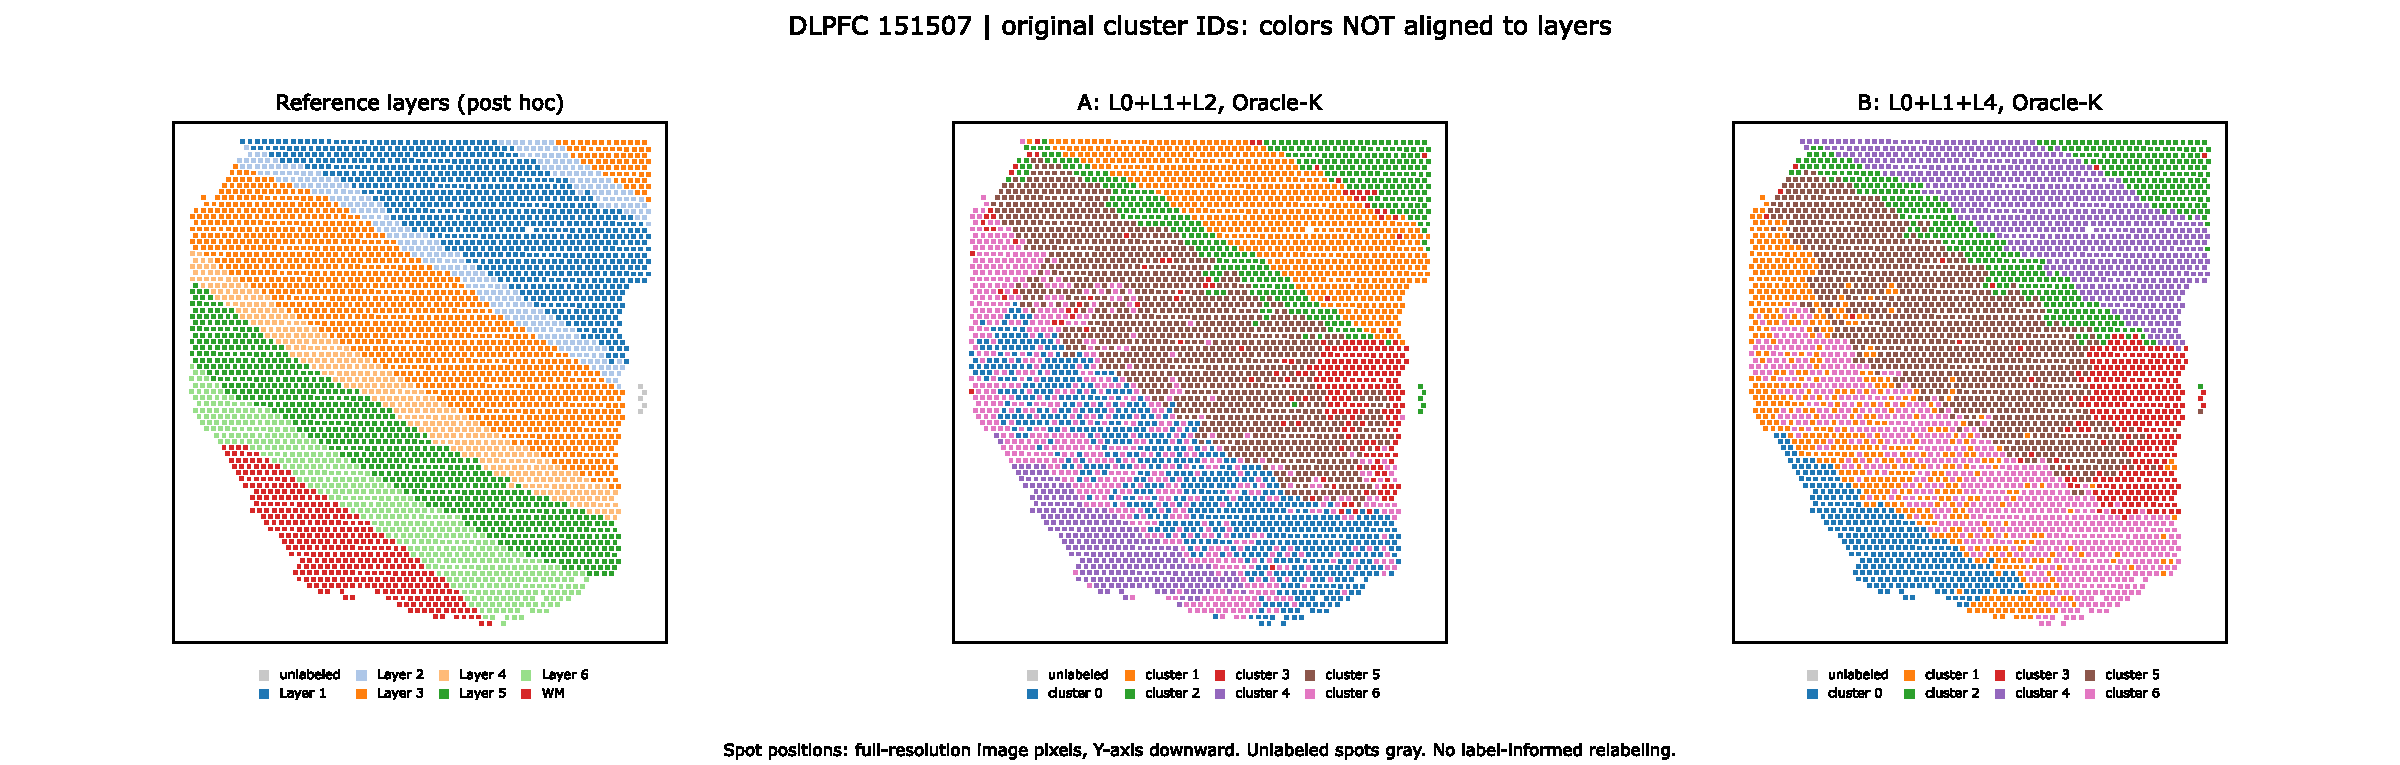
\includegraphics[width=0.98\linewidth]{E4_SOURCE_FIGURES_20261122_RELEASE/figures_pdf/151507/151507_reference_A_B_spatial.pdf}
\caption{DLPFC切片151507的参考层及A、B两种15维组合的聚类结果（第一名供体中B相对A为正向的代表切片；颜色不代表经标签对齐的簇）}
\label{fig:cc-e4-151507-p1}
\end{figure}
}{\par\noindent\emph{[编译提示：未找到151507空间三联图的PDF，请检查相对路径。]}\par}
\IfFileExists{E4_SOURCE_FIGURES_20261122_RELEASE/figures_pdf/151671/151671_reference_A_B_spatial.pdf}{%
\begin{figure}[htbp]
\centering
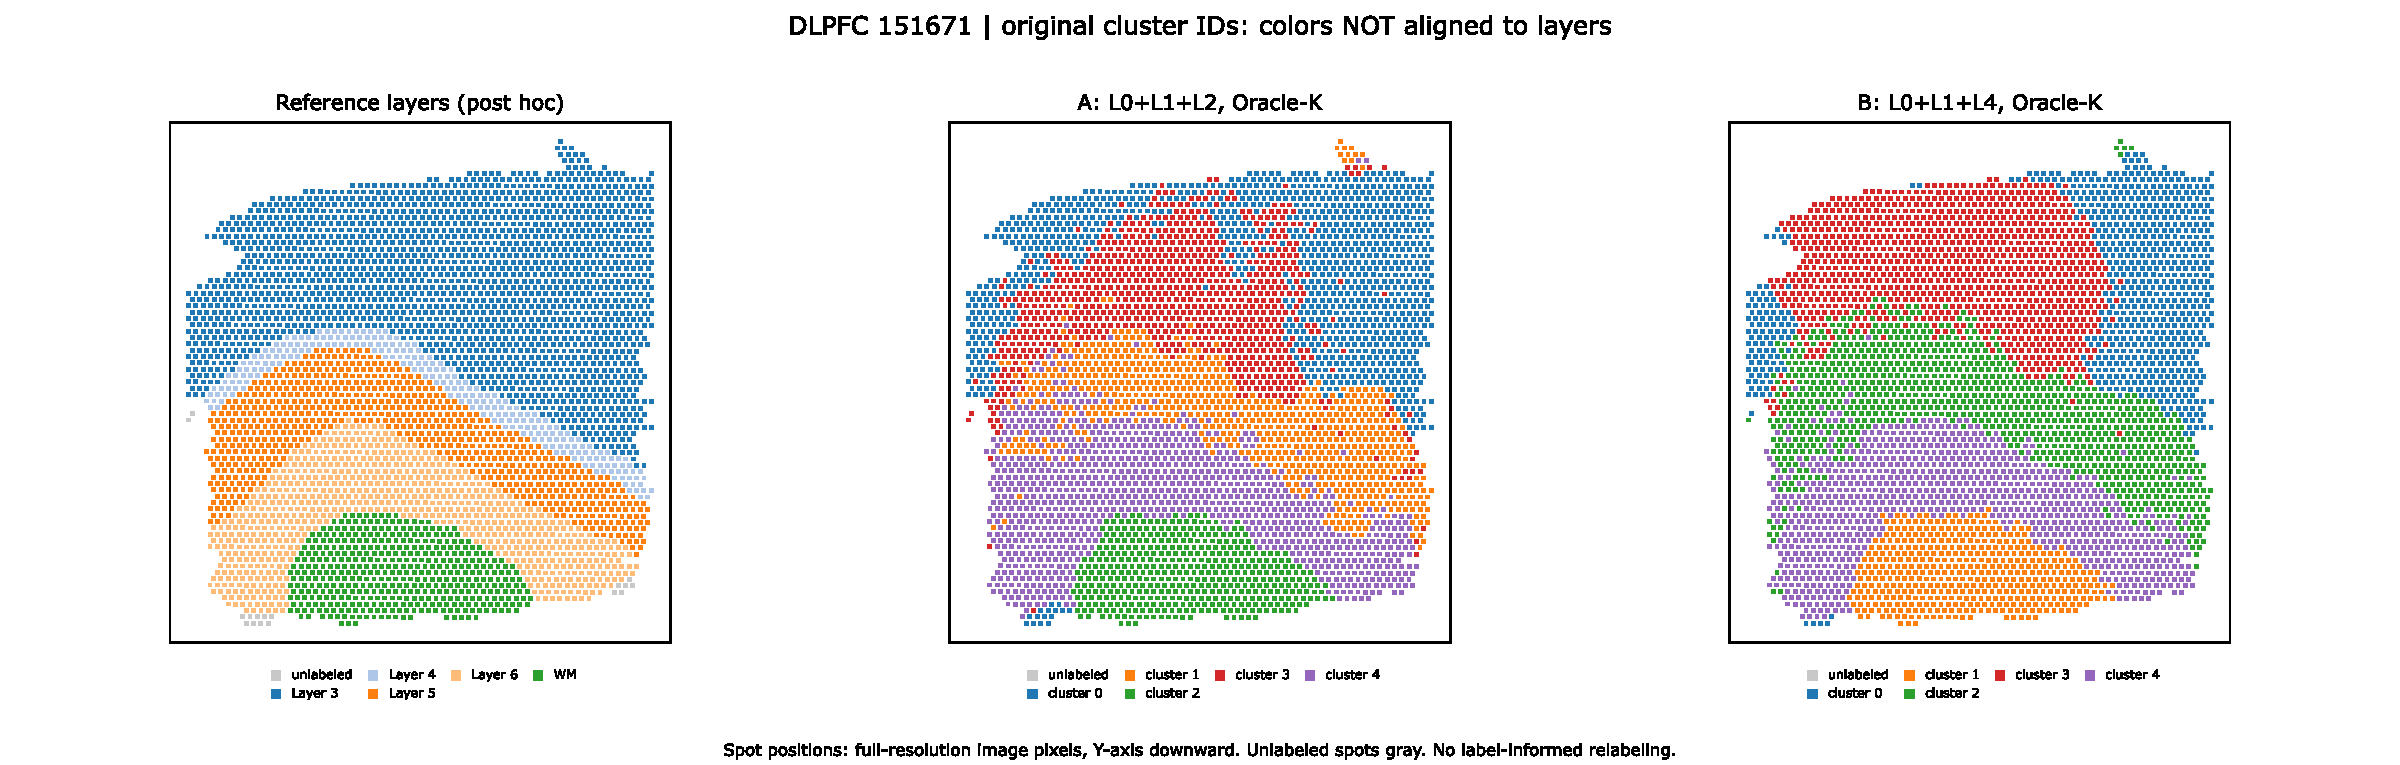
\includegraphics[width=0.98\linewidth]{E4_SOURCE_FIGURES_20261122_RELEASE/figures_pdf/151671/151671_reference_A_B_spatial.pdf}
\caption{DLPFC切片151671的参考层及A、B两种15维组合的聚类结果（第二名供体中B相对A接近零的代表切片）}
\label{fig:cc-e4-151671-p1}
\end{figure}
}{\par\noindent\emph{[编译提示：未找到151671空间三联图的PDF，请检查相对路径。]}\par}
\IfFileExists{E4_SOURCE_FIGURES_20261122_RELEASE/figures_pdf/151675/151675_reference_A_B_spatial.pdf}{%
\begin{figure}[htbp]
\centering
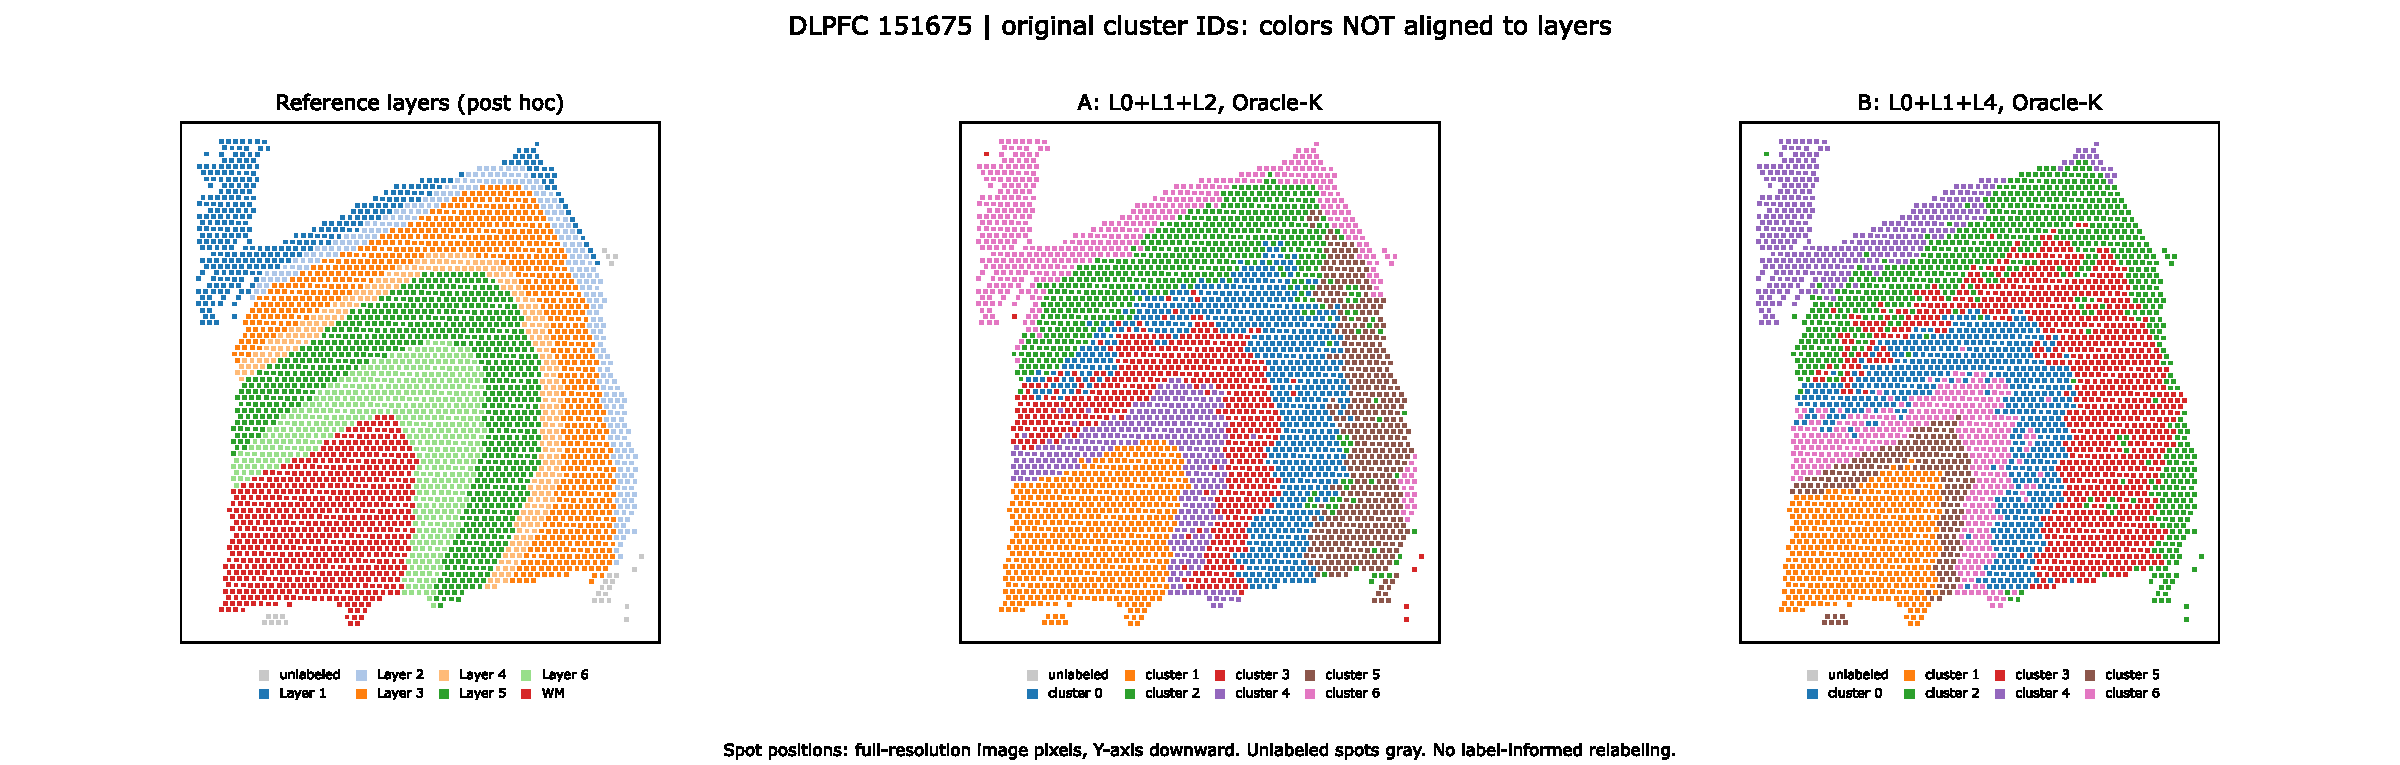
\includegraphics[width=0.98\linewidth]{E4_SOURCE_FIGURES_20261122_RELEASE/figures_pdf/151675/151675_reference_A_B_spatial.pdf}
\caption{DLPFC切片151675的参考层及A、B两种15维组合的聚类结果（第三名供体中B相对A为负向的代表切片）}
\label{fig:cc-e4-151675-p1}
\end{figure}
}{\par\noindent\emph{[编译提示：未找到151675空间三联图的PDF，请检查相对路径。]}\par}
\IfFileExists{E4_SOURCE_FIGURES_20261122_RELEASE/figures_pdf/151671/151671_MOBP_PCP4_SNAP25_expression.pdf}{%
\begin{figure}[htbp]
\centering
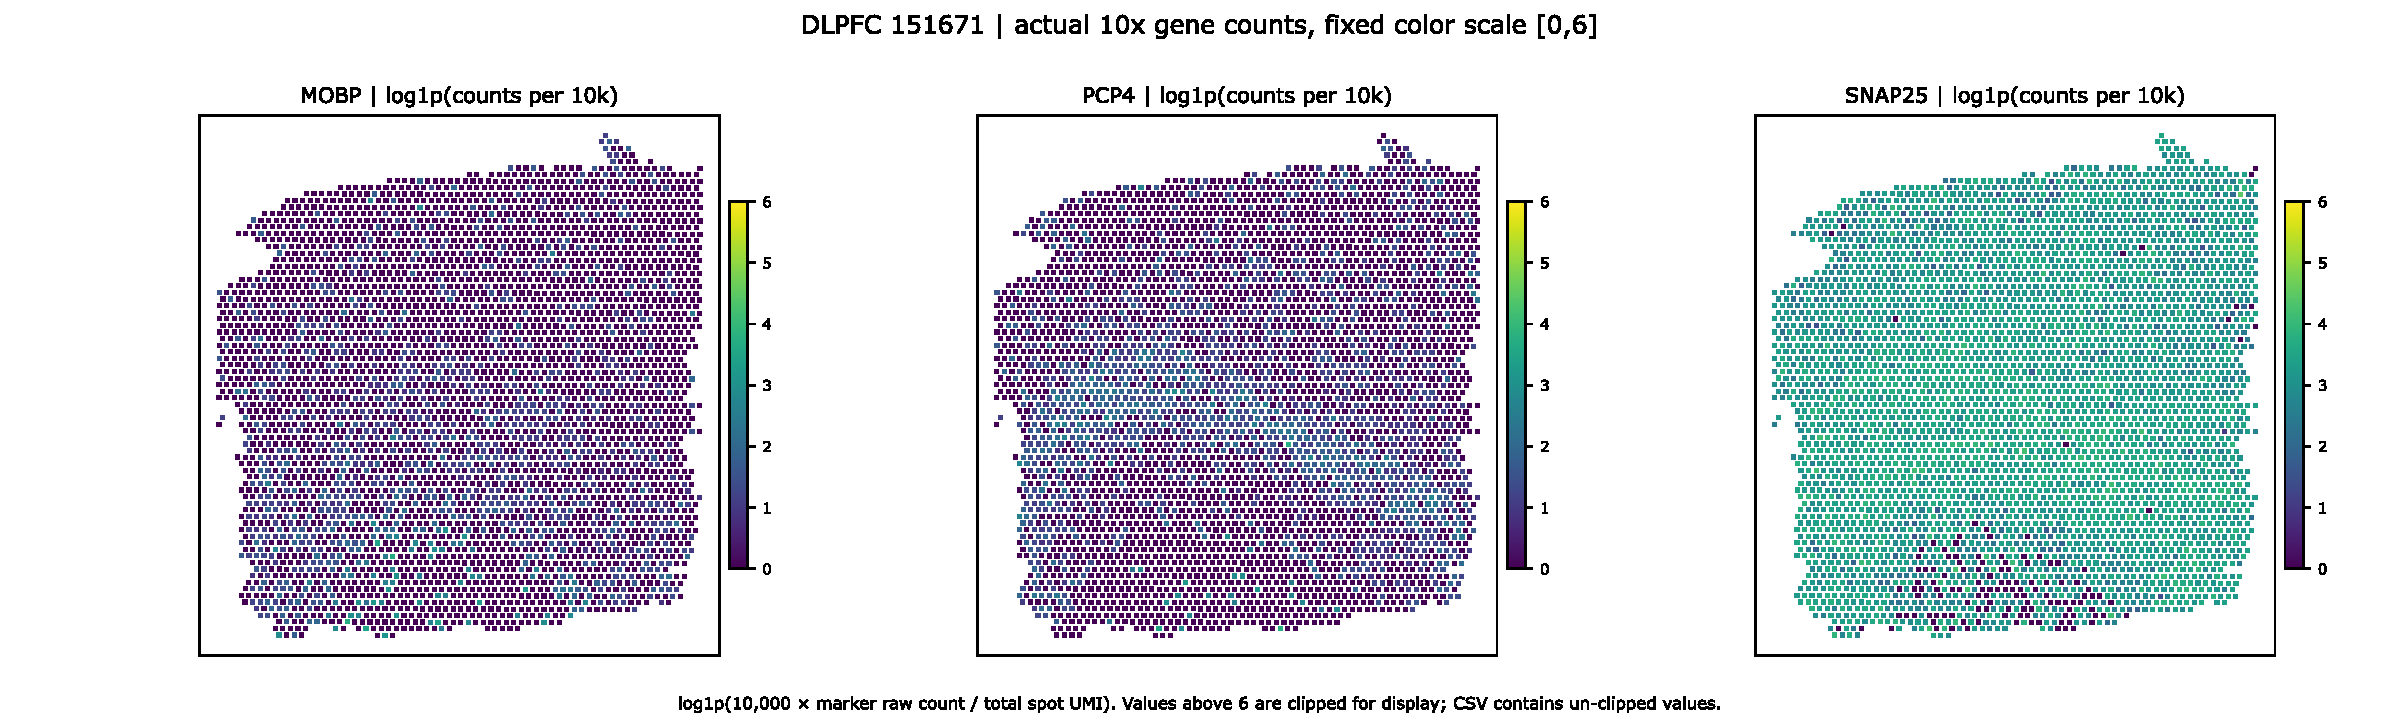
\includegraphics[width=0.98\linewidth]{E4_SOURCE_FIGURES_20261122_RELEASE/figures_pdf/151671/151671_MOBP_PCP4_SNAP25_expression.pdf}
\caption{DLPFC切片151671中MOBP、PCP4与SNAP25的归一化表达空间分布（统一的0--6色标）}
\label{fig:cc-e4-markers-151671-p1}
\end{figure}
}{\par\noindent\emph{[编译提示：未找到151671标记基因图的PDF，请检查相对路径。]}\par}

\subsection{讨论}
\label{subsec:cc-discussion-p1}

\subsubsection{同一方法的结论为何随条件而变}
以上结果显示，“邻域越大越好”这一结论只在特定的组合条件下成立：参考类别数确定K、以整体一致性或容差边界评价、观察宏平均。可以从三个方面理解其原因。
\begin{itemize}
  \item \textbf{邻域信息的边际收益递减。}一种合理的解释是：第一层邻域汇聚了相邻spot的表达，减弱了单spot表达的噪声，因此带来一致的提升；更远的邻域层与已有信息的重叠较多，增益随之变小。对于层厚不同的切片，更远的邻域还可能跨越层界，这与供体D3的反向趋势相容。以上解释都没有经过本研究的直接检验。
  \item \textbf{K的设定与尺度效应相互叠加。}固定K时，尺度排序稳定；一旦K由数据自行决定，选中K的波动（2到10）就压过了尺度之间的细小差别，排序随之改变。参考类别数并非ARI最优的K，这进一步说明，在参考类别数条件下得到的尺度比较，隐含地依赖于“K等于参考类别数”这一约定。
  \item \textbf{整体指标与严格边界指标衡量的是不同的误差。}随着邻域加深，预测边界的数量明显减少，预测分区更加平滑，整体一致性和容差边界匹配随之提高；而在严格网格匹配下，平滑后的边界只要错开一两个位置就不再计为命中，严格召回因此下降。两类指标的相反趋势，是同一组预测在不同评价问题上的表现，而不是互相矛盾的结论。
\end{itemize}

\subsubsection{对方法使用与评价的建议}
在本研究的数据与条件范围内，可以得到以下建议：
\begin{enumerate}
  \item \textbf{邻域层数。}在Visium皮层数据上，1--2层邻域已能获得大部分ARI收益；更深的聚合可以作为候选，但应报告其在切片或供体层面的方向，而不是只报告宏平均。
  \item \textbf{聚类数。}参考类别数条件下的结果应与固定K敏感性曲线一起报告。使用无标签稳定性选K时，宜采用足够的重复次数，并检查选中K是否落在搜索边界上；比较方法时，应同时列出各方法实际采用的选K规则。
  \item \textbf{边界评价。}应同时报告严格与容差边界指标，并给出precision、recall或预测边界数量，以区分定位偏移和预测碎片化。
  \item \textbf{跨数据集应用。}应逐个报告供体或患者的结果；宏平均容易被个别样本主导，在乳腺癌队列中，单个患者就足以改变配置之间的排序。
\end{enumerate}

\subsubsection{与已有研究的关系}
本研究的参考类别数结果与CellCharter原作者的单切片基准处于同一水平，也与原作者在调参中选择4层邻域相一致\cite{varrone2024}。在此基础上，本研究进一步说明：这一选择所带来的平均增益，在第一层之后已经较小，且依赖于聚类数设定和评价指标。原作者报告BIC倾向于给出更多的簇；本研究在非空间GMM基线上观察到同样的现象（32/36项选到上界）。已有的空间聚类评价研究强调，方法排序会因数据处理和参数设定而改变\cite{sun2026}；本研究在同一方法内部的尺度比较上，给出了相应的实证例子。

\subsubsection{研究局限}
\label{subsubsec:cc-limits-p1}
本研究的结论受到以下限制：
\begin{enumerate}
  \item DLPFC只有3名独立供体，乳腺癌只有6名患者，结论以描述性的分层统计为主，不作显著性推断；供体映射依据公开资料推定。
  \item 25维配置由原作者依据参考标签在3张切片上调出，组合B在开发切片上提出，这些切片都不是未接触样本；正文对相应结果分别报告了不同的汇总口径。
  \item 累计邻域深度与特征维数同时变化，等维组合只能部分区分两者的影响；边界分析没有零模型基准，相关解释不涉及因果机制。
  \item 稳定性选K只做了5次重复且逐切片运行；BayesSpace与GMM的K-blind似然规则大量命中搜索上界，其中BayesSpace的规则与官方建议不一致；对照集未包含STAGATE。这些因素限制了K-blind条件下方法比较的结论范围。
  \item 无标签选K的评分、边界指标、排除开发切片的汇总、与官方结果的对照以及K偏好分析，都是事后分析，只用于解释和检验稳健性，不是独立验证。
  \item 皮层层标注与乳腺癌病理区域的语义不同，不比较两种组织之间的ARI绝对值；外部队列的结果也不代表临床诊断性能。
\end{enumerate}

\subsection{本节小结}
本节表明，CellCharter的邻域聚合在DLPFC上带来明确的收益，收益主要集中在第一层邻域；更深的聚合只有小幅且因切片而异的增益。聚类数的设定对结论的影响大于15维之后的尺度差异，参考类别数也并非ARI最优的K。整体一致性与严格边界定位呈现相反的尺度排序，这主要源于预测碎片化程度的变化。在乳腺癌队列中，空间邻域特征相对非空间表示的收益方向得到保留，但患者间差异很大，与BayesSpace的比较随指标和K规则而变。这些结果共同说明，对成熟空间聚类方法的性能判断，应同时考虑聚类数规则、评价指标和样本层级。

\clearpage
% P1 学术写作版（2026-11-24）：结论与展望。由 cellcharter_study_conclusion_module_rev_p0_20261124.tex 改写；
% 局限的完整表述见第4.7.4节，此处只作概括。未编译。
\section{结论与展望}
\label{sec:cc-conclusion-p1}

\subsection{主要结论}
本研究以CellCharter原作者提出的方法和基准配置为基础，在3名供体的12张DLPFC切片和6例乳腺癌样本上，从邻域表征、聚类数规则、评价指标和跨组织适用性四个方面，系统评价了多尺度空间聚类的性能。主要结论如下。

\begin{enumerate}
  \item \textbf{邻域收益集中于最近邻层。}引入第一层邻域后，ARI由0.305升至0.408，并在全部切片中方向一致；15维之后的增益小于切片间差异，约半数切片和一名供体方向相反。不同15维邻域组合之间没有稳定占优者；在开发切片上提出的远邻替换组合，在其余切片和外部队列中没有复现其优势。在原作者的基准配置下，本研究结果与原作者发布的单切片结果处于同一水平。
  \item \textbf{聚类数规则对结论的影响大于深层尺度差异。}固定K时尺度排序稳定，但K本身引起的ARI变化远大于15维之后的尺度差异。参考类别数并非ARI最优的K。逐切片的无标签稳定性选K（5次重复）选出的簇数离散，并改变了尺度排序。
  \item \textbf{整体一致性与严格边界定位存在评价权衡。}随邻域加深，2-hop容差边界F1由0.286升至0.533，严格边界F1则从约0.145降至0.118。这一差异主要来自预测边界从碎片化走向平滑时召回率的变化，说明边界评价需要同时报告严格指标、容差指标及其分解。
  \item \textbf{方法比较与跨组织适用性依赖于条件。}在参考类别数条件下，CellCharter优于非空间方法和BANKSY，与BayesSpace相当；在K-blind条件下，比较结论受到各方法选K规则（包括本研究为BayesSpace和GMM设定的似然规则频繁命中上界）的强烈影响。在乳腺癌队列中，空间邻域特征相对非空间表示的收益在全部患者中方向一致，但患者间差异很大，与BayesSpace的比较随指标和K规则而变。
\end{enumerate}

综上，本研究表明：对于成熟的空间聚类方法，性能判断不能只依赖参考类别数条件下的单一整体指标，而应同时考察聚类数敏感性、严格与容差边界指标，以及供体或患者层面的结果。这为空间聚类方法的参数选择、结果解释和评价报告提供了可复核的实证依据。

\subsection{局限}
本研究的独立生物学样本较少（3名供体、6名患者），以描述性分层统计为主。部分配置所用的切片在调参或开发阶段已被分析过。邻域深度与特征维数同时变化。稳定性选K的重复次数少于原作者设定，部分基线的K-blind规则存在缺陷，对照集也未包含STAGATE。若干解释性分析属于事后分析。上述限制的完整说明见第\ref{subsubsec:cc-limits-p1}节。

\subsection{展望}
后续工作可以从以下几方面展开：
\begin{itemize}
  \item 在更多独立供体、组织类型和测序平台上检验当前结论的适用范围；
  \item 按各方法官方建议的选K方式（例如BayesSpace的拐点判断）及足够的稳定性重复次数，重新设计无标签条件下的对照，并纳入STAGATE等更强的基线；
  \item 以维度匹配的对照进一步区分邻域范围与特征维数的作用；
  \item 为边界指标建立零模型基准，并结合层间过渡区的标注不确定性完善边界评价。
\end{itemize}

\clearpage
\appendix
\IfFileExists{E4_SOURCE_FIGURES_20261122_RELEASE/figures_pdf/151507/151507_reference_A_B_spatial.pdf}{%
% P1 (2026-11-24): derived from appendix_e4_all12_figures_layout_v2_20261123.tex (unchanged).
% Changed: header, section title, intro paragraph, and missing-figure fallback text only.
% All \includegraphics paths, captions and labels are byte-identical to layout V2.
\section{全部12张DLPFC切片的空间分布图件}
\label{sec:cc-e4-appendix-v1}
本附录列出全部12张DLPFC切片的空间聚类图、标记基因表达图与参考层--聚类交叉计数图，作为第\ref{subsec:cc-res-maps-p1}节的完整补充。所有图件均使用随机种子22911、参考类别数条件下A、B两种15维组合的原始预测；聚类编号未依据参考标签重排。12张切片来自3名供体，不构成12个独立的生物学重复。图件由原始计数与预测直接绘制，未作任何重绘或生成式处理。

\subsection{DLPFC切片151507}
\IfFileExists{E4_SOURCE_FIGURES_20261122_RELEASE/figures_pdf/151507/151507_reference_A_B_spatial.pdf}{%
\par\noindent\begin{minipage}{\linewidth}
\centering
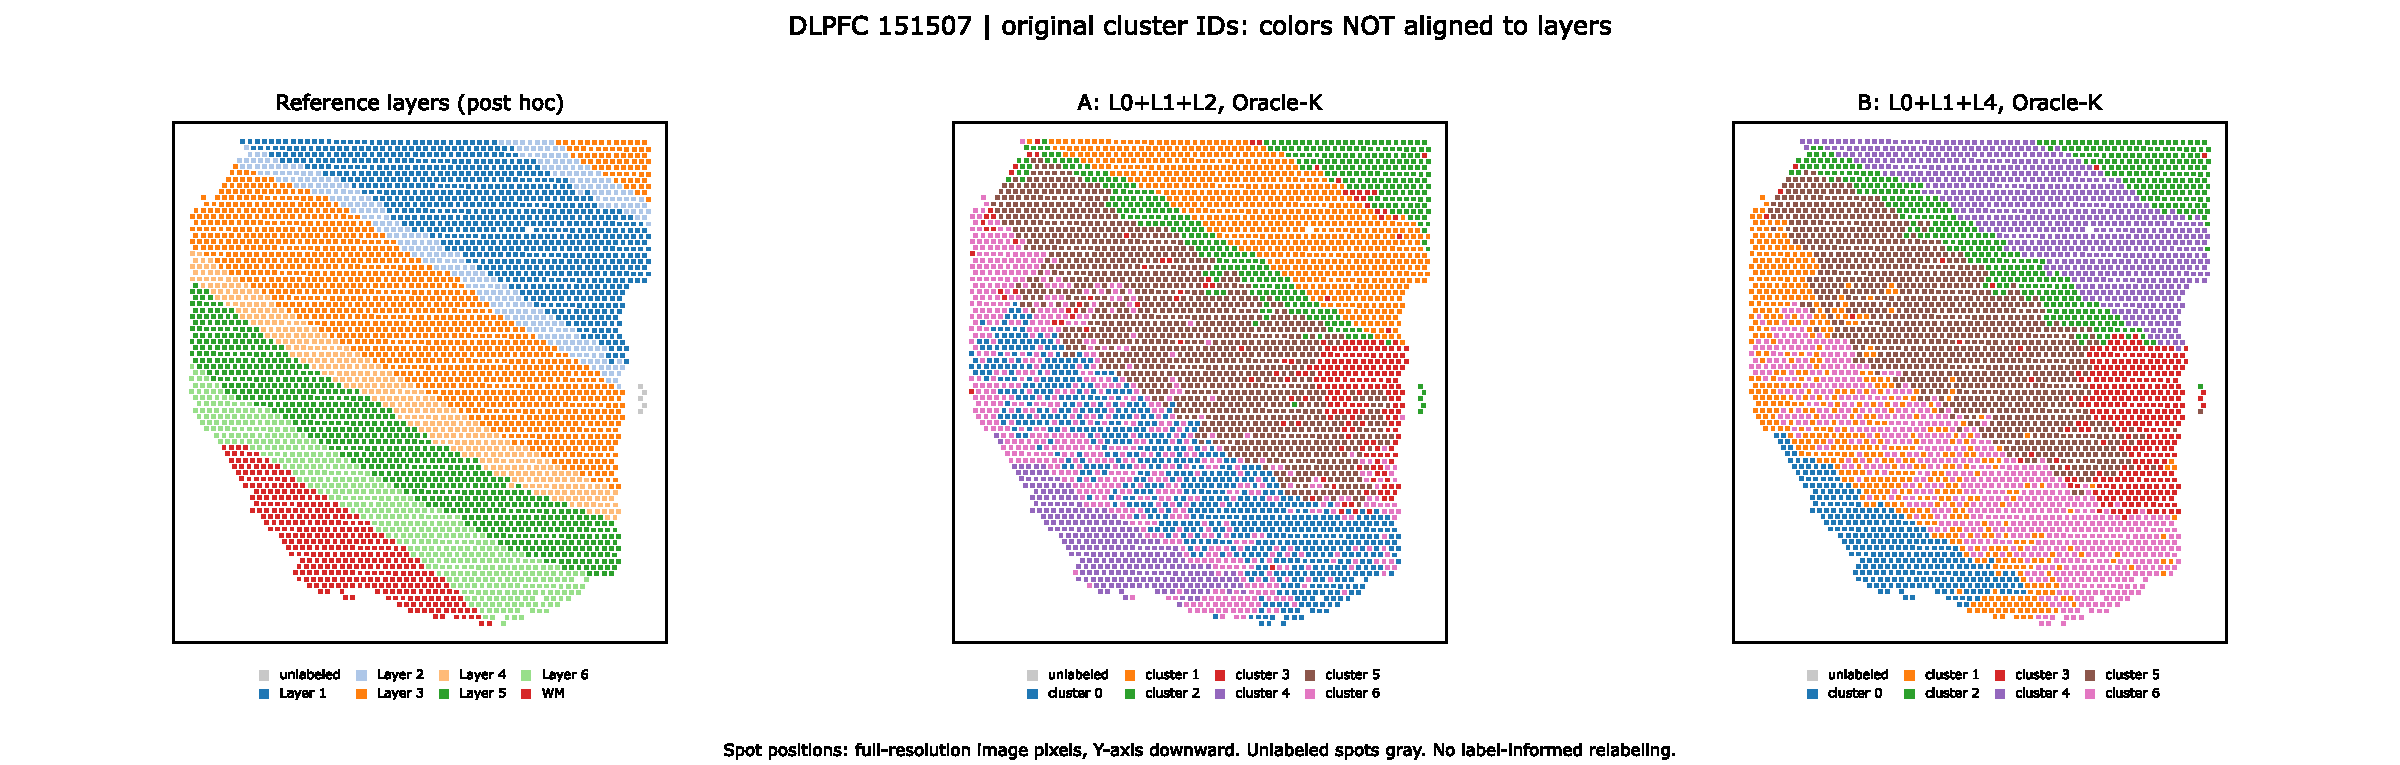
\includegraphics[width=0.97\linewidth,height=0.72\textheight,keepaspectratio]{E4_SOURCE_FIGURES_20261122_RELEASE/figures_pdf/151507/151507_reference_A_B_spatial.pdf}
\captionof{figure}{DLPFC切片151507：参考层与A/B原始聚类三联图（原始E4图件转换的矢量PDF；聚类编号未根据参考标签重排）。}
\label{fig:cc-e4-app-151507-map}
\end{minipage}\par\medskip
}{%
\par\noindent\emph{[编译提示：未找到该图件的PDF，请检查相对路径。]}\par
}
\IfFileExists{E4_SOURCE_FIGURES_20261122_RELEASE/figures_pdf/151507/151507_MOBP_PCP4_SNAP25_expression.pdf}{%
\par\noindent\begin{minipage}{\linewidth}
\centering
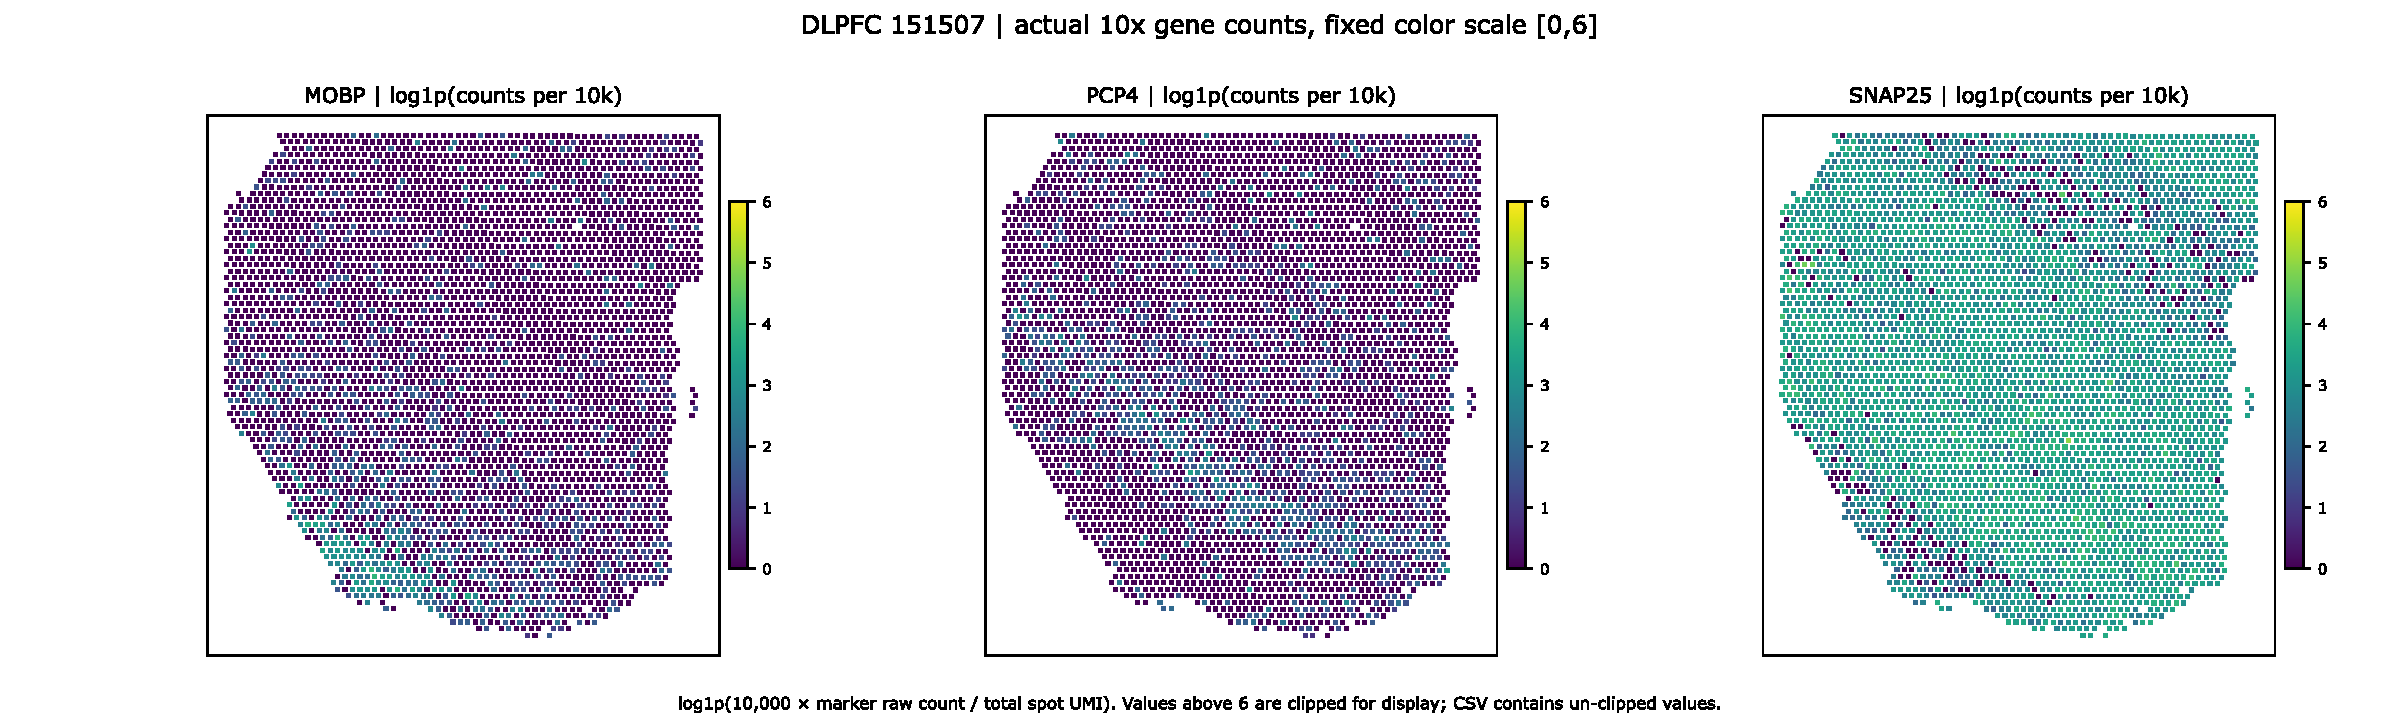
\includegraphics[width=0.97\linewidth,height=0.72\textheight,keepaspectratio]{E4_SOURCE_FIGURES_20261122_RELEASE/figures_pdf/151507/151507_MOBP_PCP4_SNAP25_expression.pdf}
\captionof{figure}{DLPFC切片151507：MOBP/PCP4/SNAP25表达三联图（原始E4图件转换的矢量PDF；聚类编号未根据参考标签重排）。}
\label{fig:cc-e4-app-151507-markers}
\end{minipage}\par\medskip
}{%
\par\noindent\emph{[编译提示：未找到该图件的PDF，请检查相对路径。]}\par
}
\IfFileExists{E4_SOURCE_FIGURES_20261122_RELEASE/figures_pdf/151507/151507_reference_A_B_confusion.pdf}{%
\par\noindent\begin{minipage}{\linewidth}
\centering
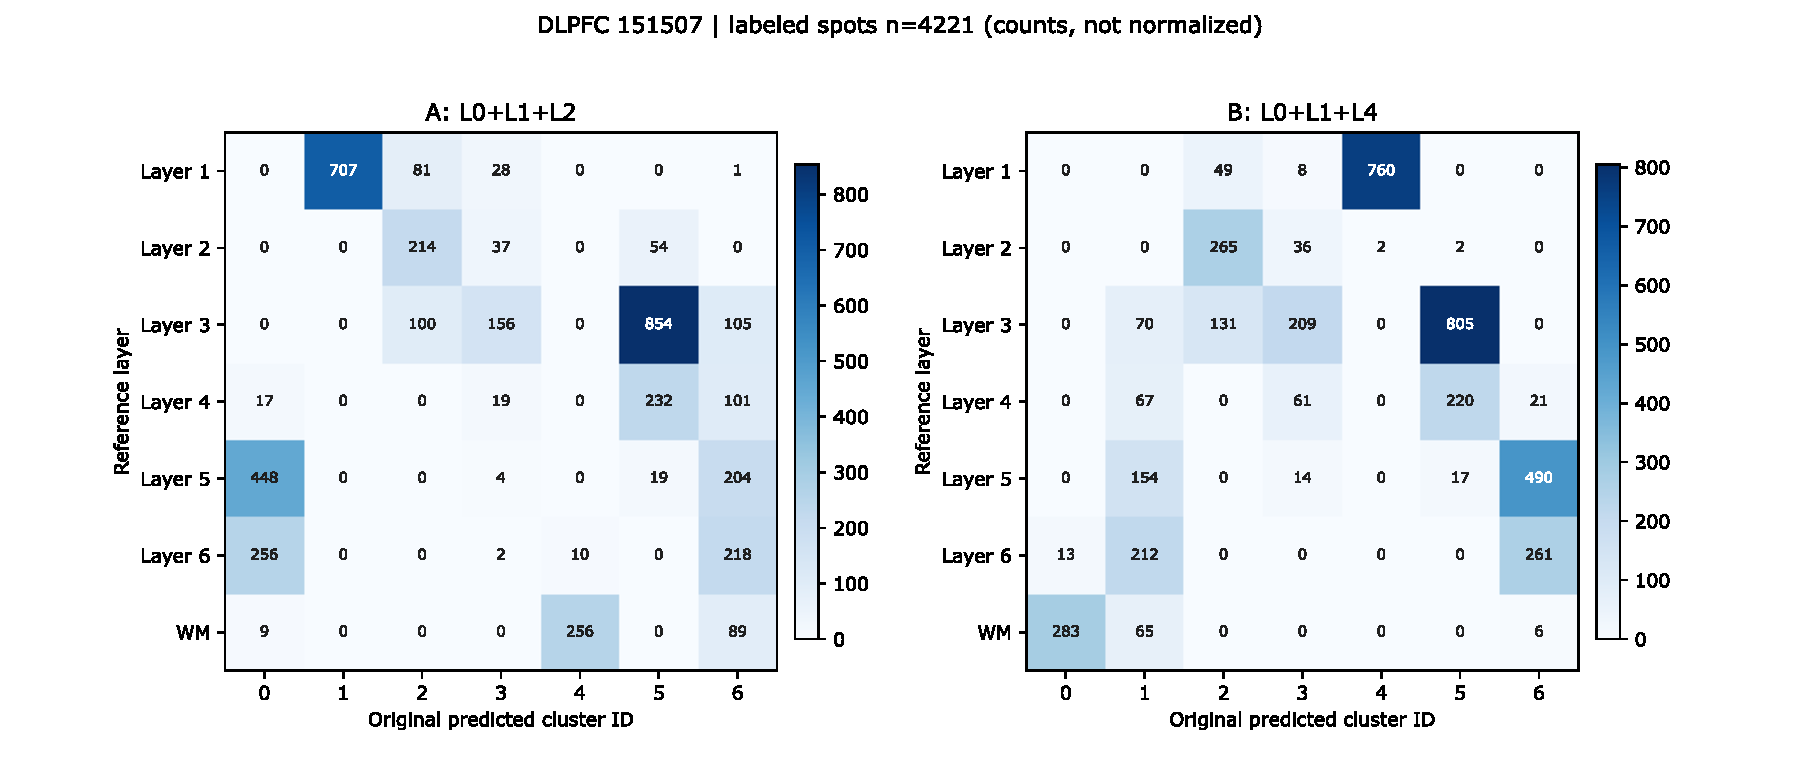
\includegraphics[width=0.97\linewidth,height=0.72\textheight,keepaspectratio]{E4_SOURCE_FIGURES_20261122_RELEASE/figures_pdf/151507/151507_reference_A_B_confusion.pdf}
\captionof{figure}{DLPFC切片151507：参考层与A/B簇交叉计数图（原始E4图件转换的矢量PDF；聚类编号未根据参考标签重排）。}
\label{fig:cc-e4-app-151507-confusion}
\end{minipage}\par\medskip
}{%
\par\noindent\emph{[编译提示：未找到该图件的PDF，请检查相对路径。]}\par
}
\subsection{DLPFC切片151508}
\IfFileExists{E4_SOURCE_FIGURES_20261122_RELEASE/figures_pdf/151508/151508_reference_A_B_spatial.pdf}{%
\par\noindent\begin{minipage}{\linewidth}
\centering
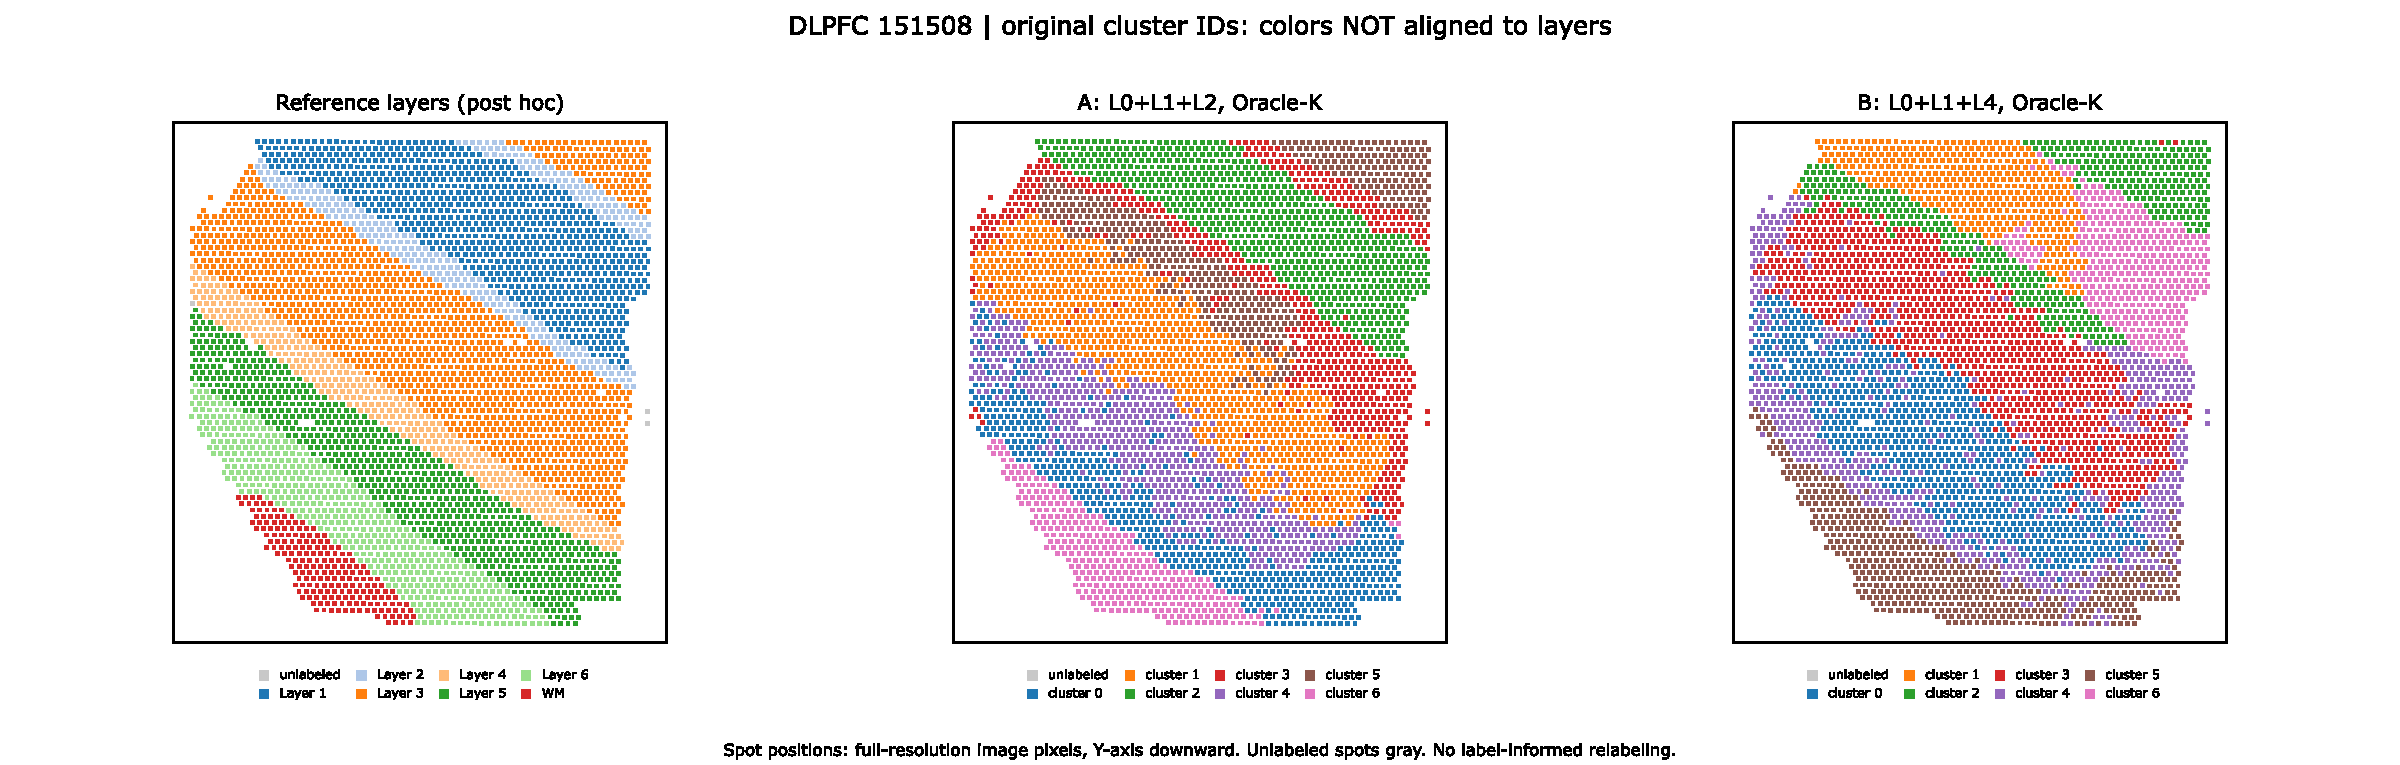
\includegraphics[width=0.97\linewidth,height=0.72\textheight,keepaspectratio]{E4_SOURCE_FIGURES_20261122_RELEASE/figures_pdf/151508/151508_reference_A_B_spatial.pdf}
\captionof{figure}{DLPFC切片151508：参考层与A/B原始聚类三联图（原始E4图件转换的矢量PDF；聚类编号未根据参考标签重排）。}
\label{fig:cc-e4-app-151508-map}
\end{minipage}\par\medskip
}{%
\par\noindent\emph{[编译提示：未找到该图件的PDF，请检查相对路径。]}\par
}
\IfFileExists{E4_SOURCE_FIGURES_20261122_RELEASE/figures_pdf/151508/151508_MOBP_PCP4_SNAP25_expression.pdf}{%
\par\noindent\begin{minipage}{\linewidth}
\centering
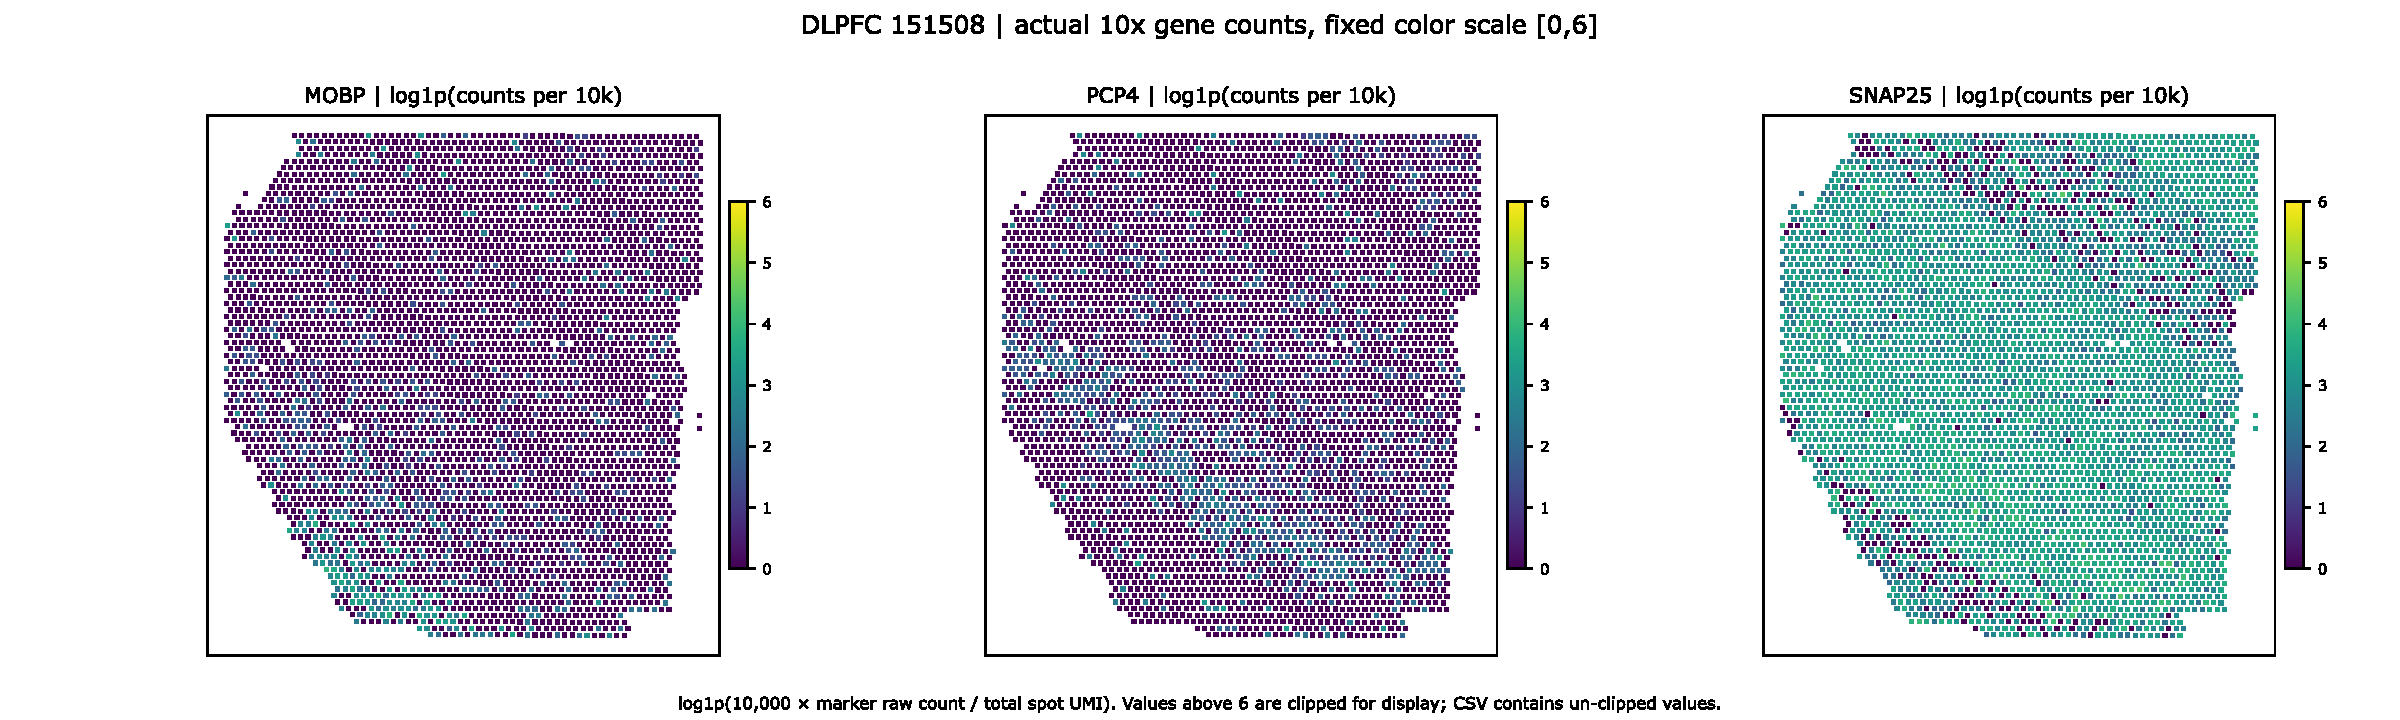
\includegraphics[width=0.97\linewidth,height=0.72\textheight,keepaspectratio]{E4_SOURCE_FIGURES_20261122_RELEASE/figures_pdf/151508/151508_MOBP_PCP4_SNAP25_expression.pdf}
\captionof{figure}{DLPFC切片151508：MOBP/PCP4/SNAP25表达三联图（原始E4图件转换的矢量PDF；聚类编号未根据参考标签重排）。}
\label{fig:cc-e4-app-151508-markers}
\end{minipage}\par\medskip
}{%
\par\noindent\emph{[编译提示：未找到该图件的PDF，请检查相对路径。]}\par
}
\IfFileExists{E4_SOURCE_FIGURES_20261122_RELEASE/figures_pdf/151508/151508_reference_A_B_confusion.pdf}{%
\par\noindent\begin{minipage}{\linewidth}
\centering
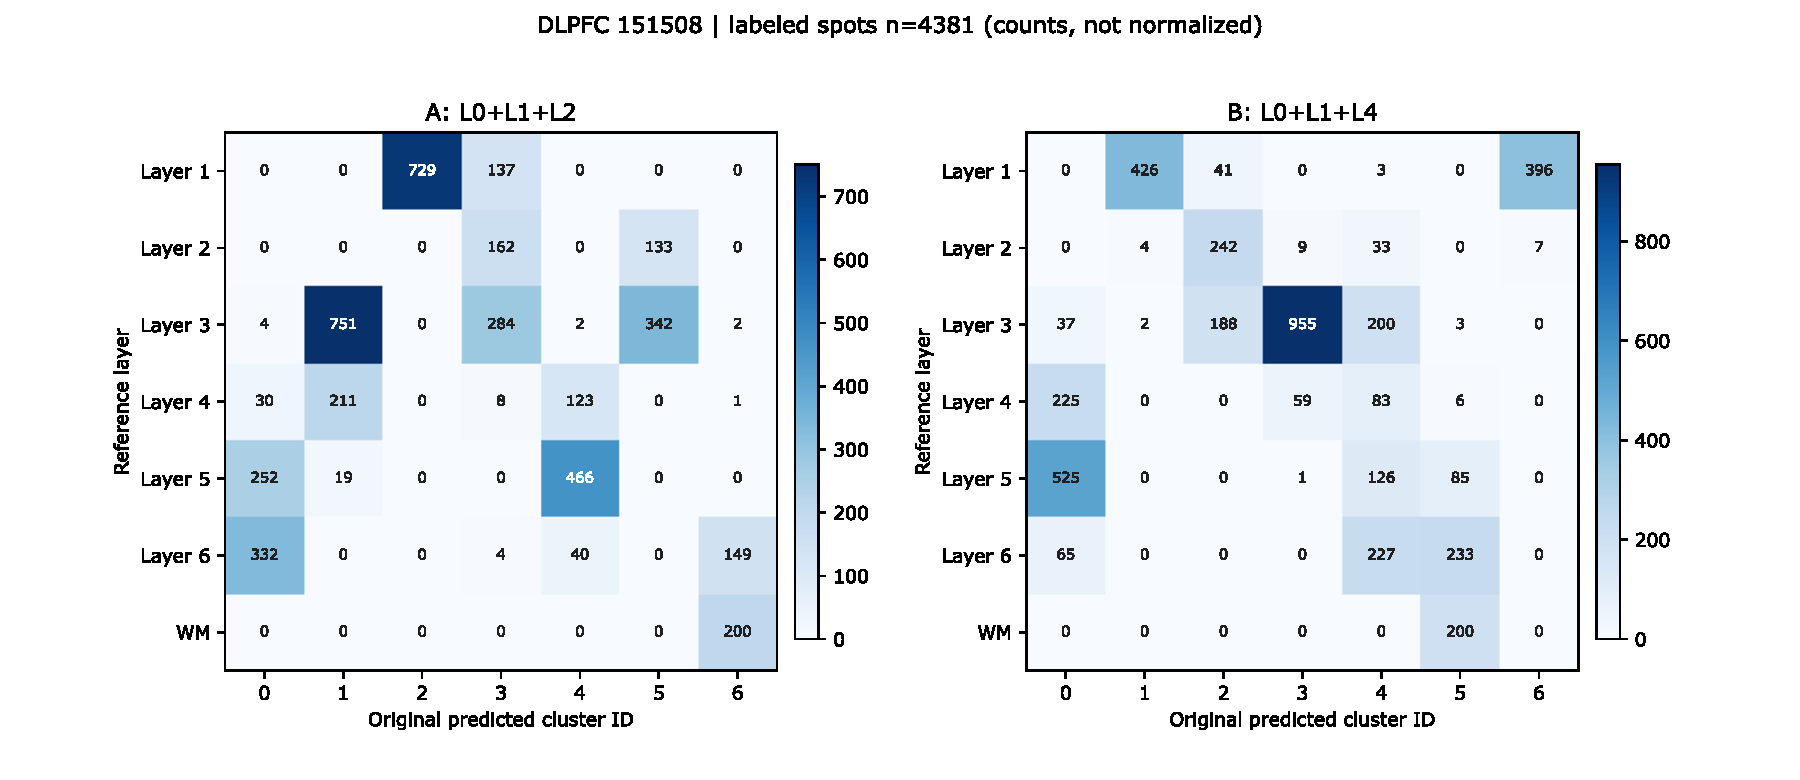
\includegraphics[width=0.97\linewidth,height=0.72\textheight,keepaspectratio]{E4_SOURCE_FIGURES_20261122_RELEASE/figures_pdf/151508/151508_reference_A_B_confusion.pdf}
\captionof{figure}{DLPFC切片151508：参考层与A/B簇交叉计数图（原始E4图件转换的矢量PDF；聚类编号未根据参考标签重排）。}
\label{fig:cc-e4-app-151508-confusion}
\end{minipage}\par\medskip
}{%
\par\noindent\emph{[编译提示：未找到该图件的PDF，请检查相对路径。]}\par
}
\subsection{DLPFC切片151509}
\IfFileExists{E4_SOURCE_FIGURES_20261122_RELEASE/figures_pdf/151509/151509_reference_A_B_spatial.pdf}{%
\par\noindent\begin{minipage}{\linewidth}
\centering
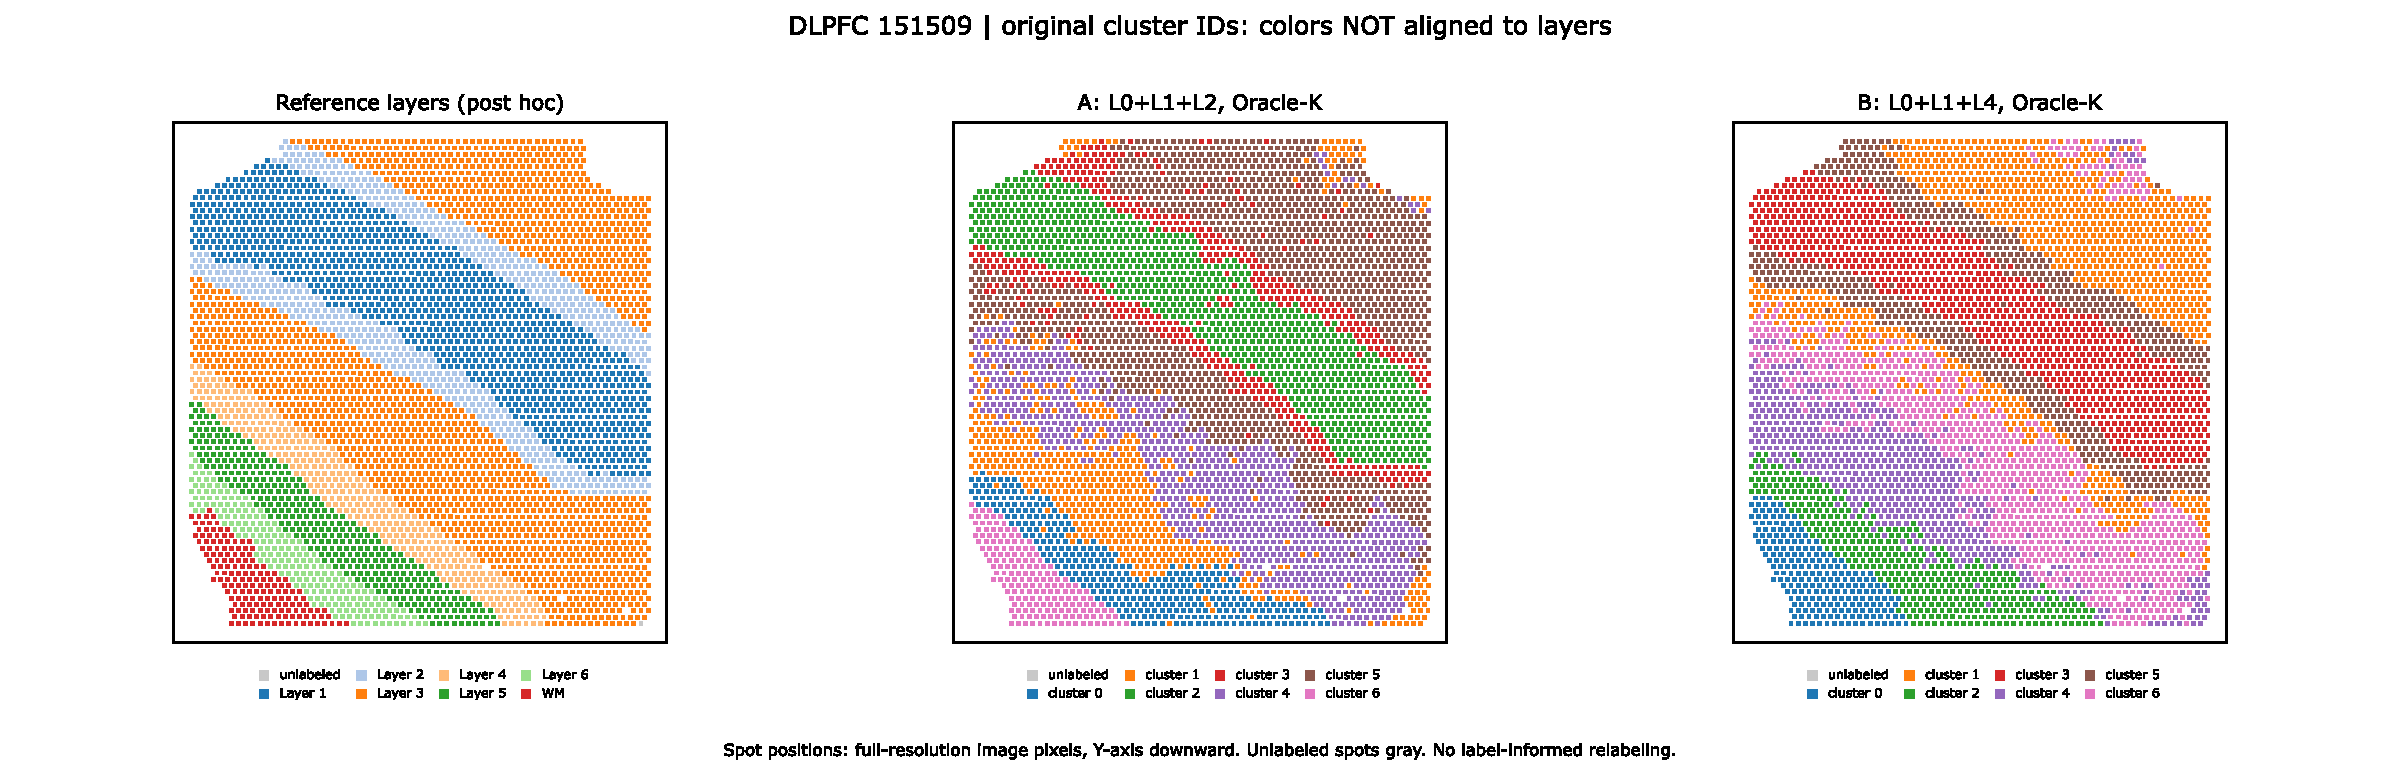
\includegraphics[width=0.97\linewidth,height=0.72\textheight,keepaspectratio]{E4_SOURCE_FIGURES_20261122_RELEASE/figures_pdf/151509/151509_reference_A_B_spatial.pdf}
\captionof{figure}{DLPFC切片151509：参考层与A/B原始聚类三联图（原始E4图件转换的矢量PDF；聚类编号未根据参考标签重排）。}
\label{fig:cc-e4-app-151509-map}
\end{minipage}\par\medskip
}{%
\par\noindent\emph{[编译提示：未找到该图件的PDF，请检查相对路径。]}\par
}
\IfFileExists{E4_SOURCE_FIGURES_20261122_RELEASE/figures_pdf/151509/151509_MOBP_PCP4_SNAP25_expression.pdf}{%
\par\noindent\begin{minipage}{\linewidth}
\centering
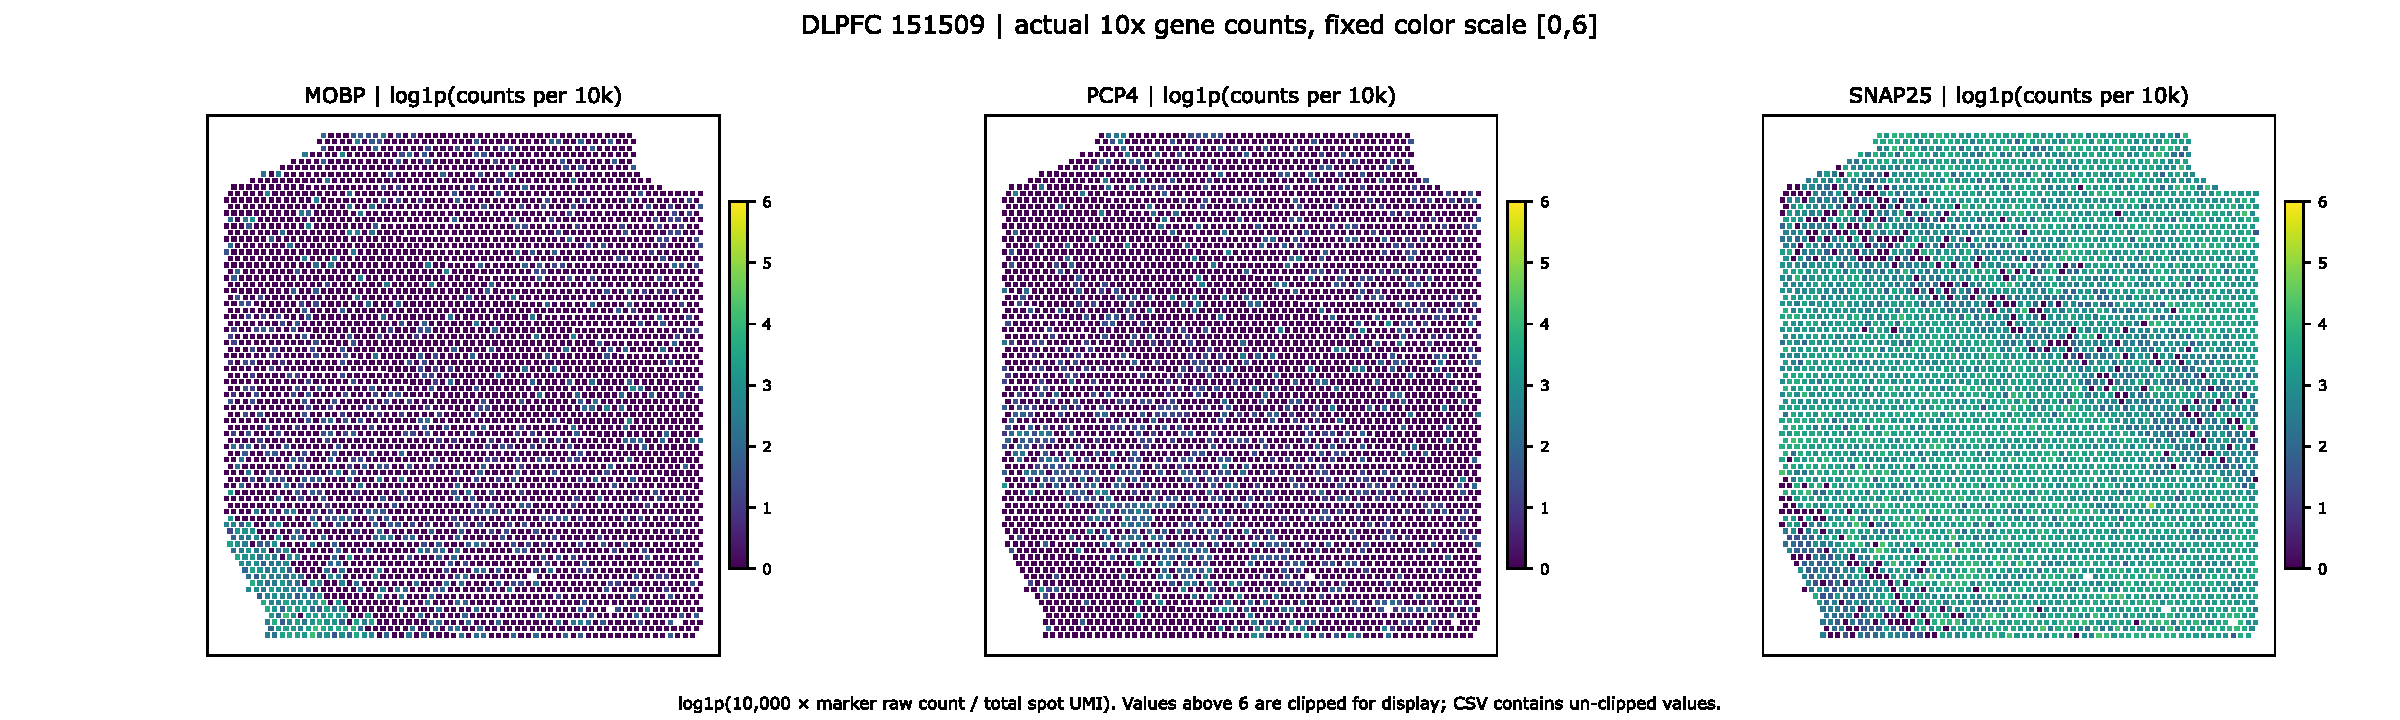
\includegraphics[width=0.97\linewidth,height=0.72\textheight,keepaspectratio]{E4_SOURCE_FIGURES_20261122_RELEASE/figures_pdf/151509/151509_MOBP_PCP4_SNAP25_expression.pdf}
\captionof{figure}{DLPFC切片151509：MOBP/PCP4/SNAP25表达三联图（原始E4图件转换的矢量PDF；聚类编号未根据参考标签重排）。}
\label{fig:cc-e4-app-151509-markers}
\end{minipage}\par\medskip
}{%
\par\noindent\emph{[编译提示：未找到该图件的PDF，请检查相对路径。]}\par
}
\IfFileExists{E4_SOURCE_FIGURES_20261122_RELEASE/figures_pdf/151509/151509_reference_A_B_confusion.pdf}{%
\par\noindent\begin{minipage}{\linewidth}
\centering
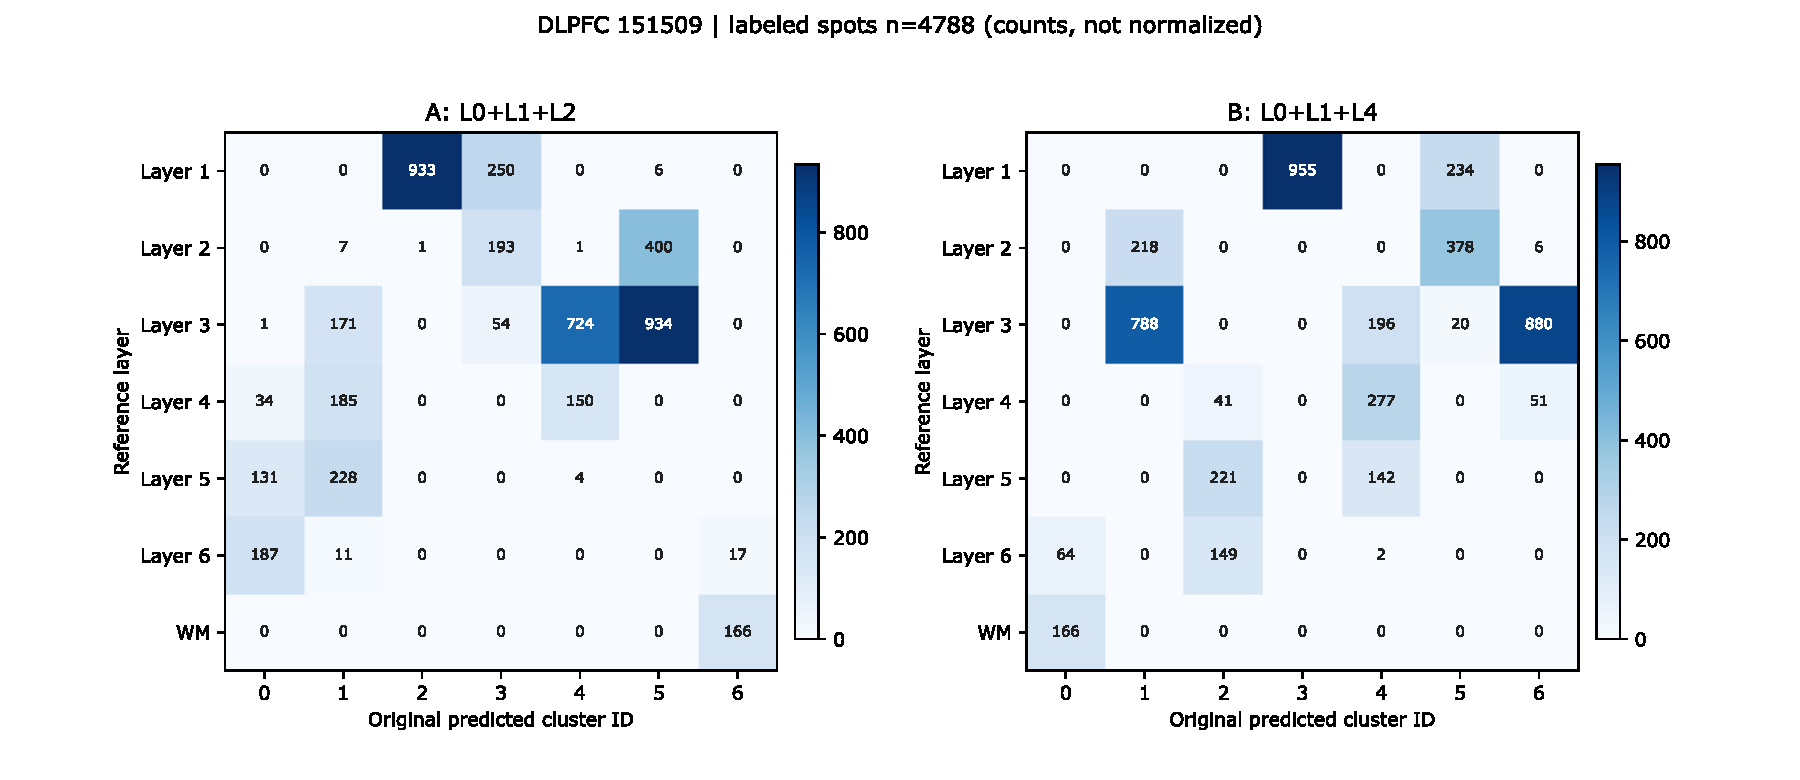
\includegraphics[width=0.97\linewidth,height=0.72\textheight,keepaspectratio]{E4_SOURCE_FIGURES_20261122_RELEASE/figures_pdf/151509/151509_reference_A_B_confusion.pdf}
\captionof{figure}{DLPFC切片151509：参考层与A/B簇交叉计数图（原始E4图件转换的矢量PDF；聚类编号未根据参考标签重排）。}
\label{fig:cc-e4-app-151509-confusion}
\end{minipage}\par\medskip
}{%
\par\noindent\emph{[编译提示：未找到该图件的PDF，请检查相对路径。]}\par
}
\subsection{DLPFC切片151510}
\IfFileExists{E4_SOURCE_FIGURES_20261122_RELEASE/figures_pdf/151510/151510_reference_A_B_spatial.pdf}{%
\par\noindent\begin{minipage}{\linewidth}
\centering
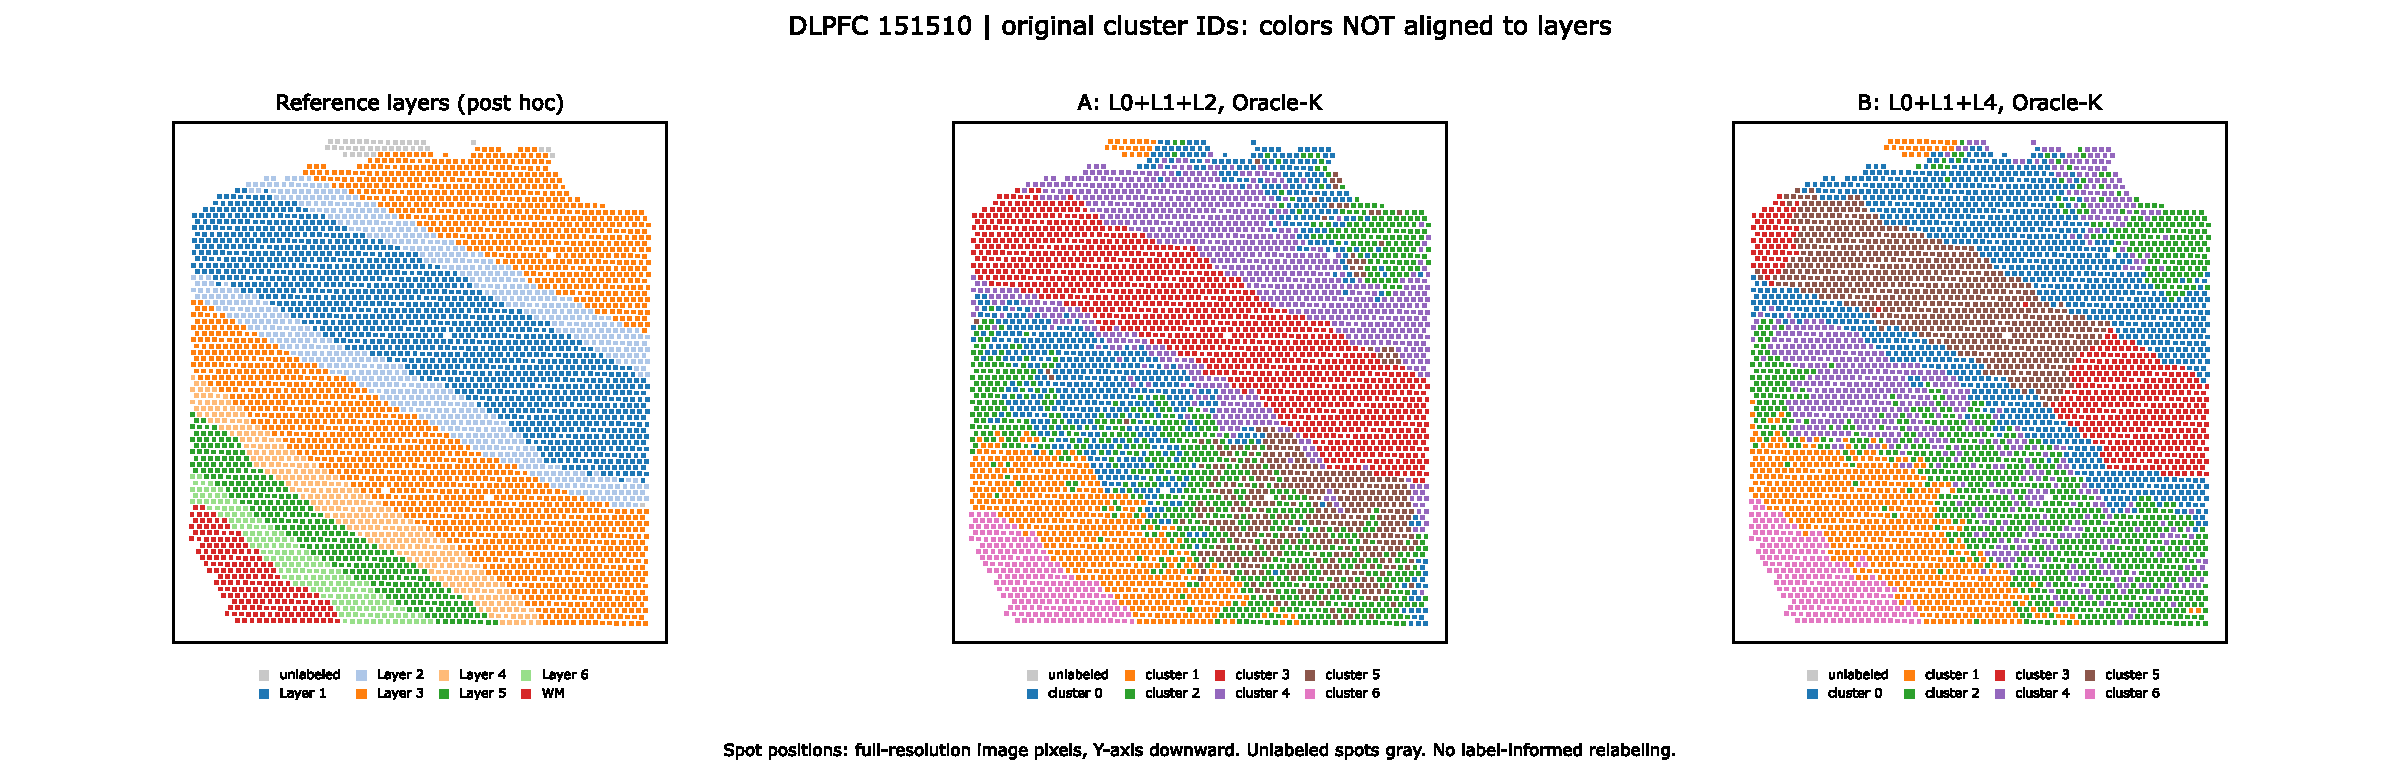
\includegraphics[width=0.97\linewidth,height=0.72\textheight,keepaspectratio]{E4_SOURCE_FIGURES_20261122_RELEASE/figures_pdf/151510/151510_reference_A_B_spatial.pdf}
\captionof{figure}{DLPFC切片151510：参考层与A/B原始聚类三联图（原始E4图件转换的矢量PDF；聚类编号未根据参考标签重排）。}
\label{fig:cc-e4-app-151510-map}
\end{minipage}\par\medskip
}{%
\par\noindent\emph{[编译提示：未找到该图件的PDF，请检查相对路径。]}\par
}
\IfFileExists{E4_SOURCE_FIGURES_20261122_RELEASE/figures_pdf/151510/151510_MOBP_PCP4_SNAP25_expression.pdf}{%
\par\noindent\begin{minipage}{\linewidth}
\centering
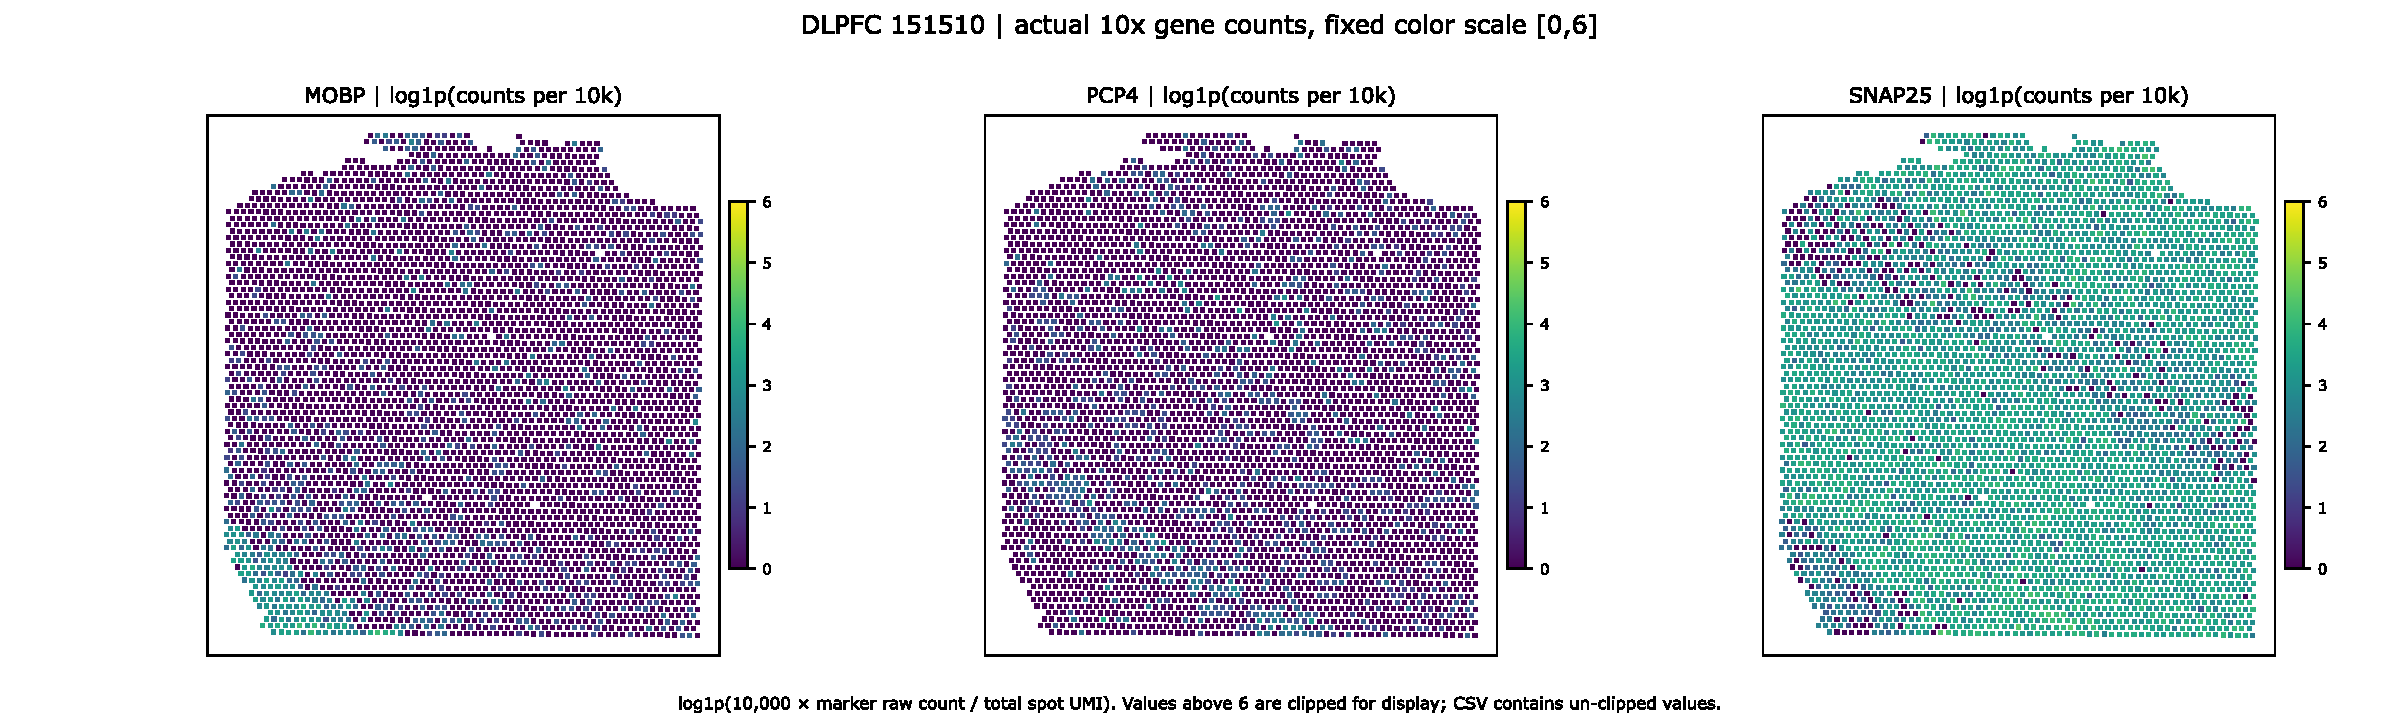
\includegraphics[width=0.97\linewidth,height=0.72\textheight,keepaspectratio]{E4_SOURCE_FIGURES_20261122_RELEASE/figures_pdf/151510/151510_MOBP_PCP4_SNAP25_expression.pdf}
\captionof{figure}{DLPFC切片151510：MOBP/PCP4/SNAP25表达三联图（原始E4图件转换的矢量PDF；聚类编号未根据参考标签重排）。}
\label{fig:cc-e4-app-151510-markers}
\end{minipage}\par\medskip
}{%
\par\noindent\emph{[编译提示：未找到该图件的PDF，请检查相对路径。]}\par
}
\IfFileExists{E4_SOURCE_FIGURES_20261122_RELEASE/figures_pdf/151510/151510_reference_A_B_confusion.pdf}{%
\par\noindent\begin{minipage}{\linewidth}
\centering
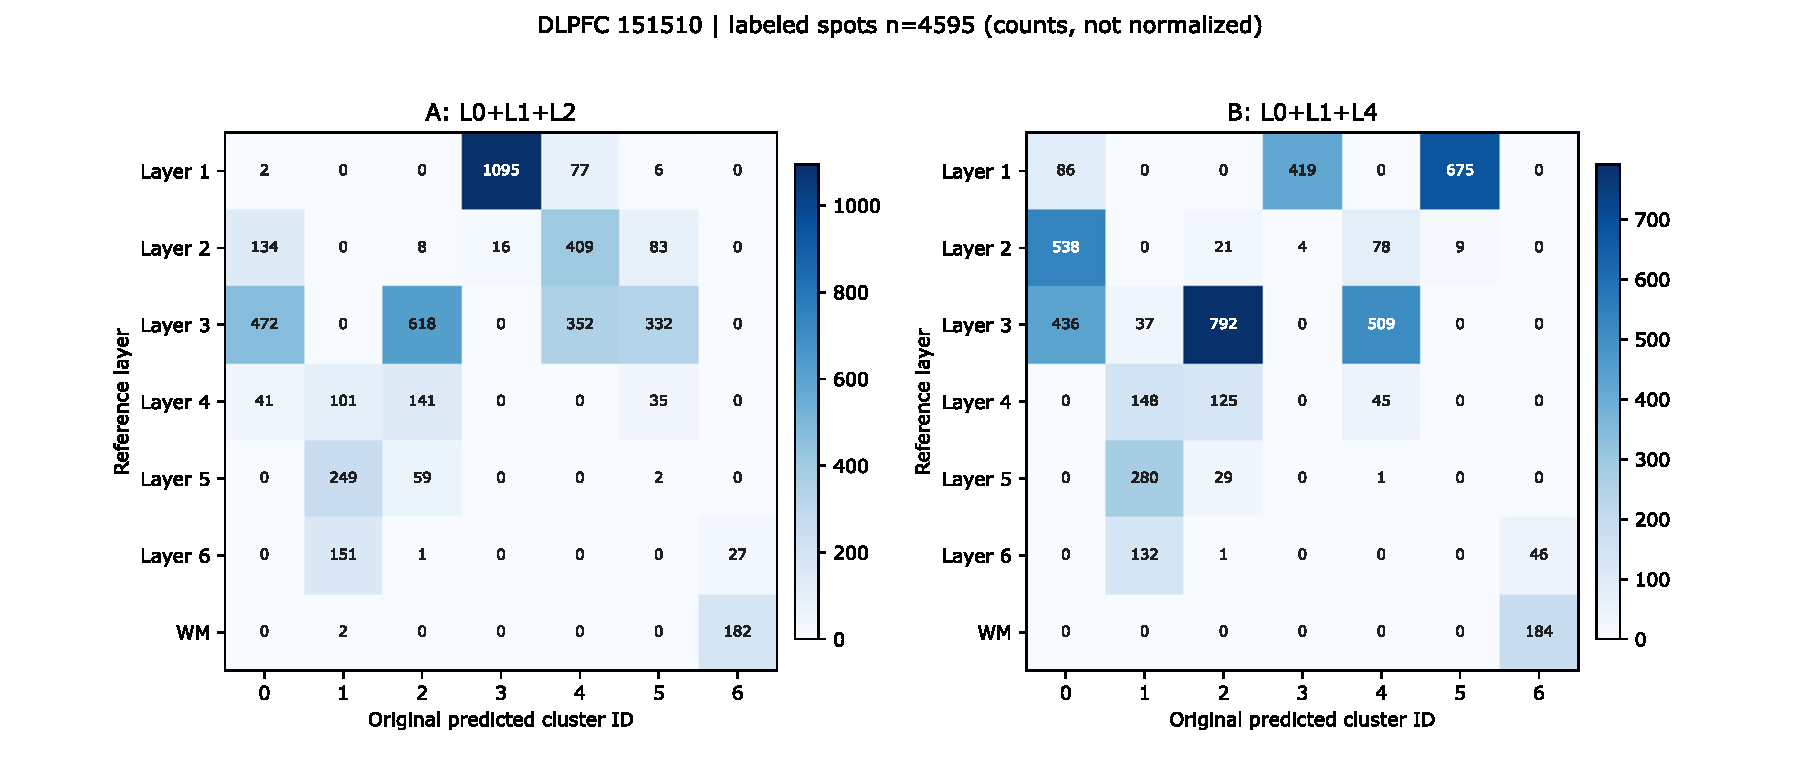
\includegraphics[width=0.97\linewidth,height=0.72\textheight,keepaspectratio]{E4_SOURCE_FIGURES_20261122_RELEASE/figures_pdf/151510/151510_reference_A_B_confusion.pdf}
\captionof{figure}{DLPFC切片151510：参考层与A/B簇交叉计数图（原始E4图件转换的矢量PDF；聚类编号未根据参考标签重排）。}
\label{fig:cc-e4-app-151510-confusion}
\end{minipage}\par\medskip
}{%
\par\noindent\emph{[编译提示：未找到该图件的PDF，请检查相对路径。]}\par
}
\subsection{DLPFC切片151669}
\IfFileExists{E4_SOURCE_FIGURES_20261122_RELEASE/figures_pdf/151669/151669_reference_A_B_spatial.pdf}{%
\par\noindent\begin{minipage}{\linewidth}
\centering
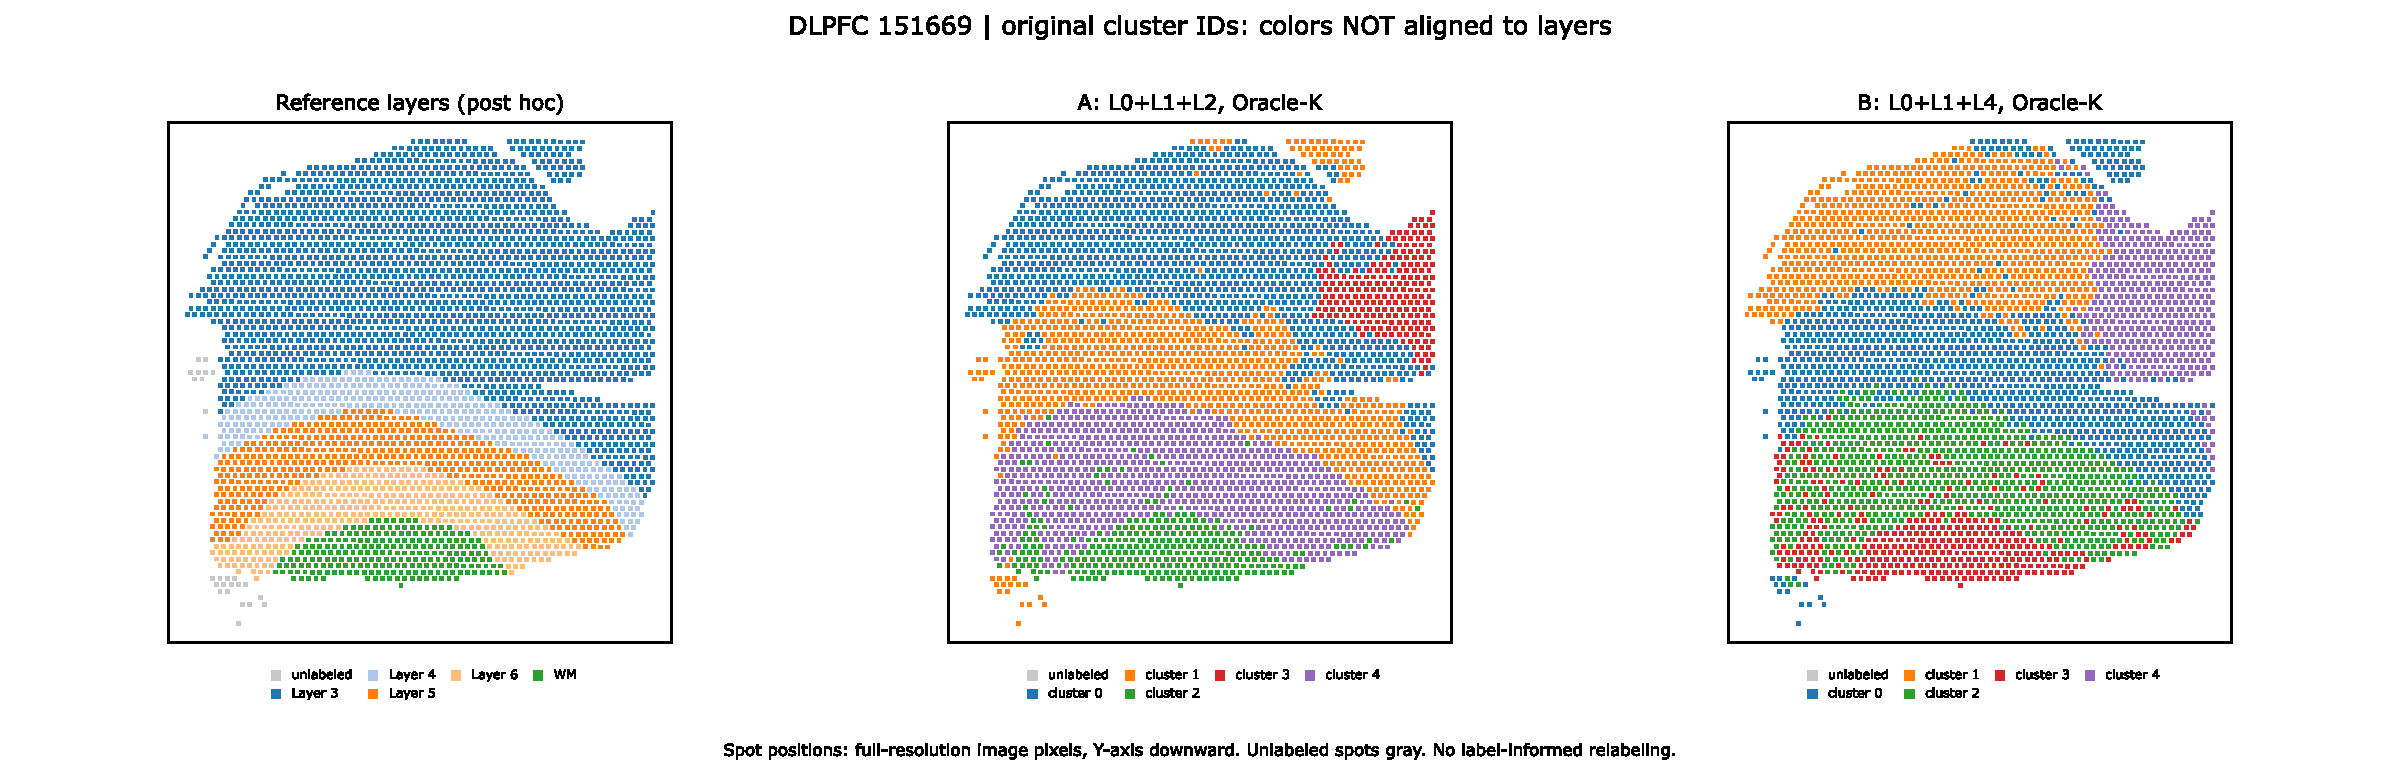
\includegraphics[width=0.97\linewidth,height=0.72\textheight,keepaspectratio]{E4_SOURCE_FIGURES_20261122_RELEASE/figures_pdf/151669/151669_reference_A_B_spatial.pdf}
\captionof{figure}{DLPFC切片151669：参考层与A/B原始聚类三联图（原始E4图件转换的矢量PDF；聚类编号未根据参考标签重排）。}
\label{fig:cc-e4-app-151669-map}
\end{minipage}\par\medskip
}{%
\par\noindent\emph{[编译提示：未找到该图件的PDF，请检查相对路径。]}\par
}
\IfFileExists{E4_SOURCE_FIGURES_20261122_RELEASE/figures_pdf/151669/151669_MOBP_PCP4_SNAP25_expression.pdf}{%
\par\noindent\begin{minipage}{\linewidth}
\centering
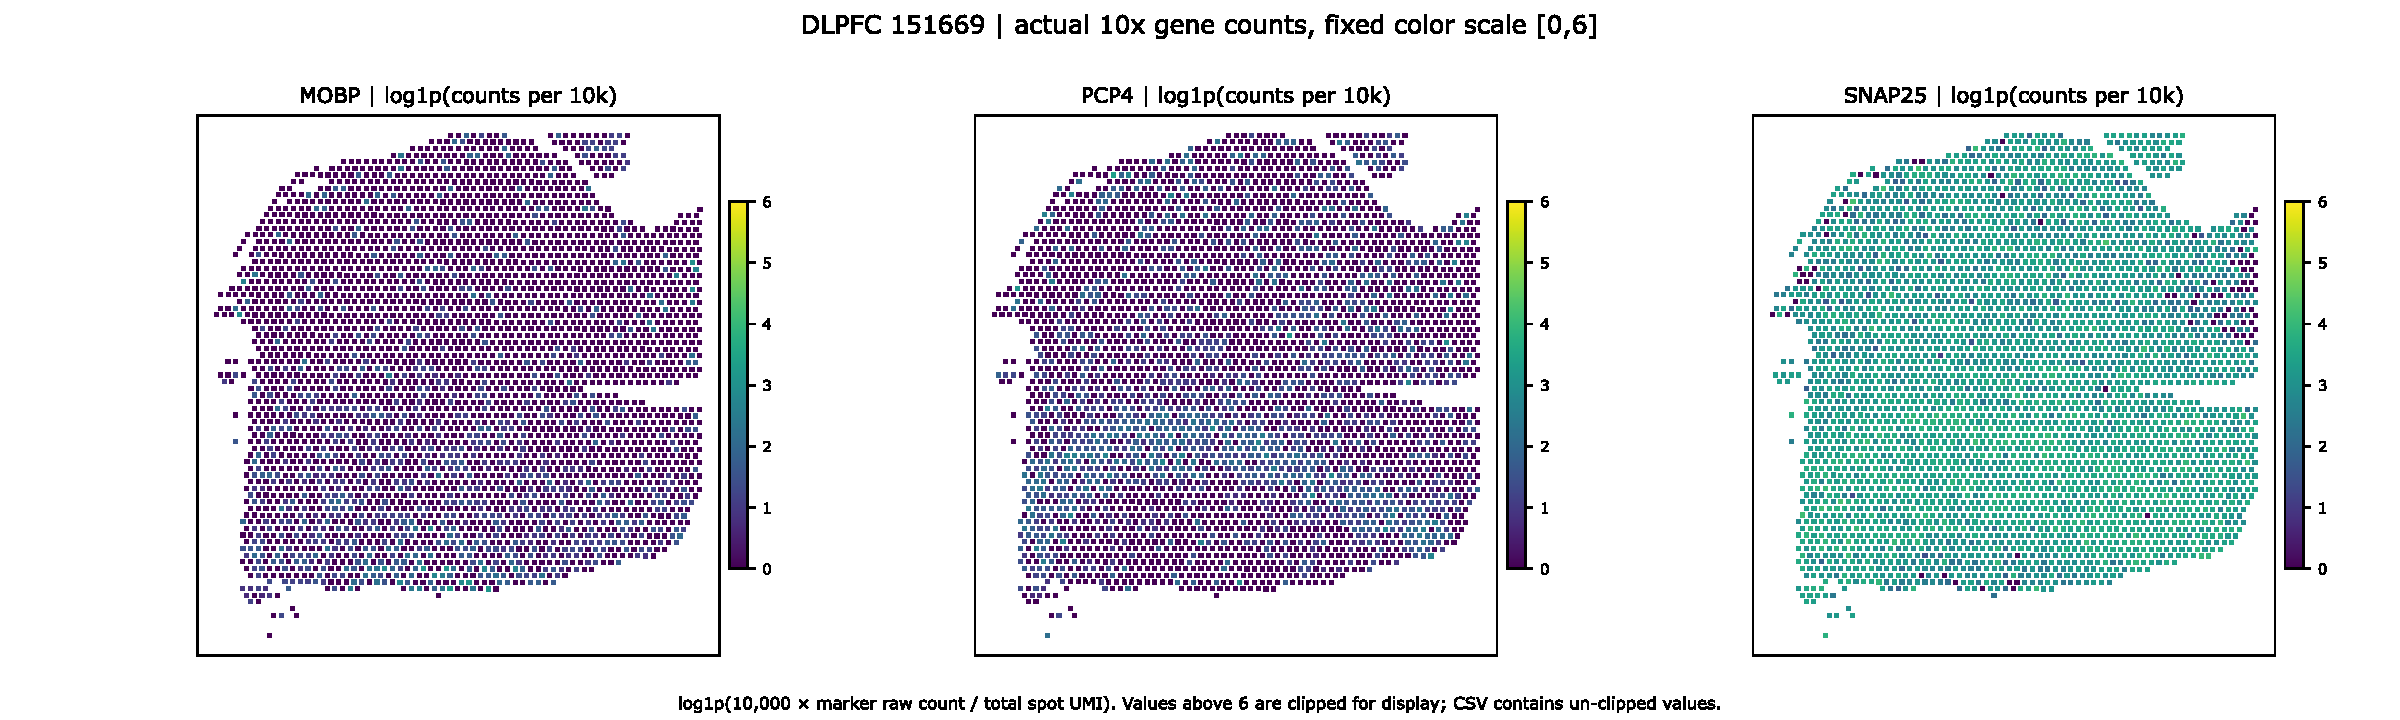
\includegraphics[width=0.97\linewidth,height=0.72\textheight,keepaspectratio]{E4_SOURCE_FIGURES_20261122_RELEASE/figures_pdf/151669/151669_MOBP_PCP4_SNAP25_expression.pdf}
\captionof{figure}{DLPFC切片151669：MOBP/PCP4/SNAP25表达三联图（原始E4图件转换的矢量PDF；聚类编号未根据参考标签重排）。}
\label{fig:cc-e4-app-151669-markers}
\end{minipage}\par\medskip
}{%
\par\noindent\emph{[编译提示：未找到该图件的PDF，请检查相对路径。]}\par
}
\IfFileExists{E4_SOURCE_FIGURES_20261122_RELEASE/figures_pdf/151669/151669_reference_A_B_confusion.pdf}{%
\par\noindent\begin{minipage}{\linewidth}
\centering
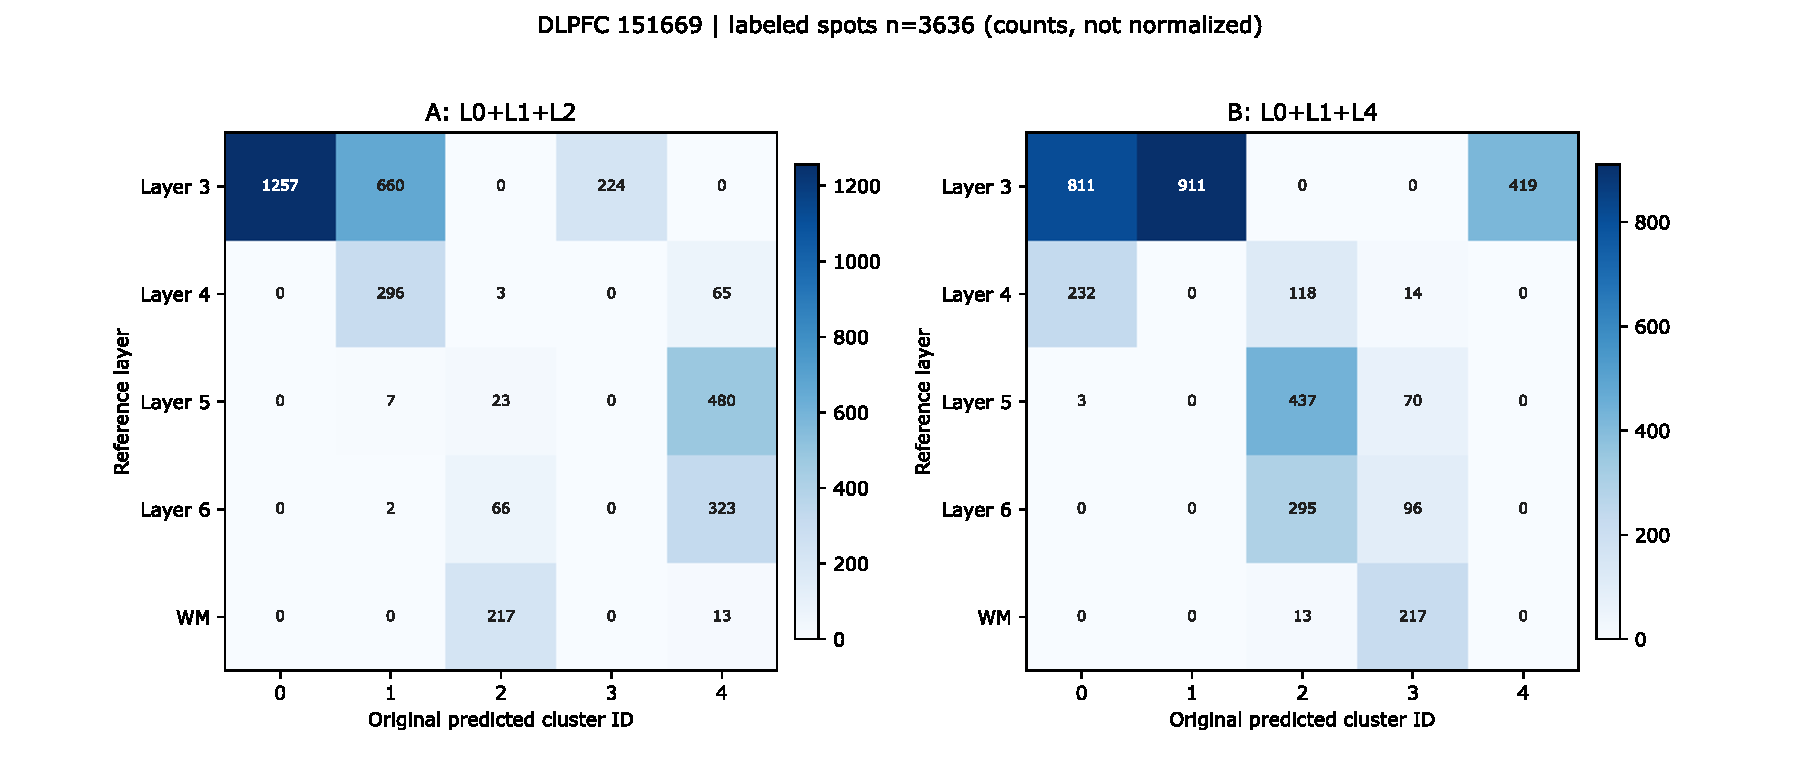
\includegraphics[width=0.97\linewidth,height=0.72\textheight,keepaspectratio]{E4_SOURCE_FIGURES_20261122_RELEASE/figures_pdf/151669/151669_reference_A_B_confusion.pdf}
\captionof{figure}{DLPFC切片151669：参考层与A/B簇交叉计数图（原始E4图件转换的矢量PDF；聚类编号未根据参考标签重排）。}
\label{fig:cc-e4-app-151669-confusion}
\end{minipage}\par\medskip
}{%
\par\noindent\emph{[编译提示：未找到该图件的PDF，请检查相对路径。]}\par
}
\subsection{DLPFC切片151670}
\IfFileExists{E4_SOURCE_FIGURES_20261122_RELEASE/figures_pdf/151670/151670_reference_A_B_spatial.pdf}{%
\par\noindent\begin{minipage}{\linewidth}
\centering
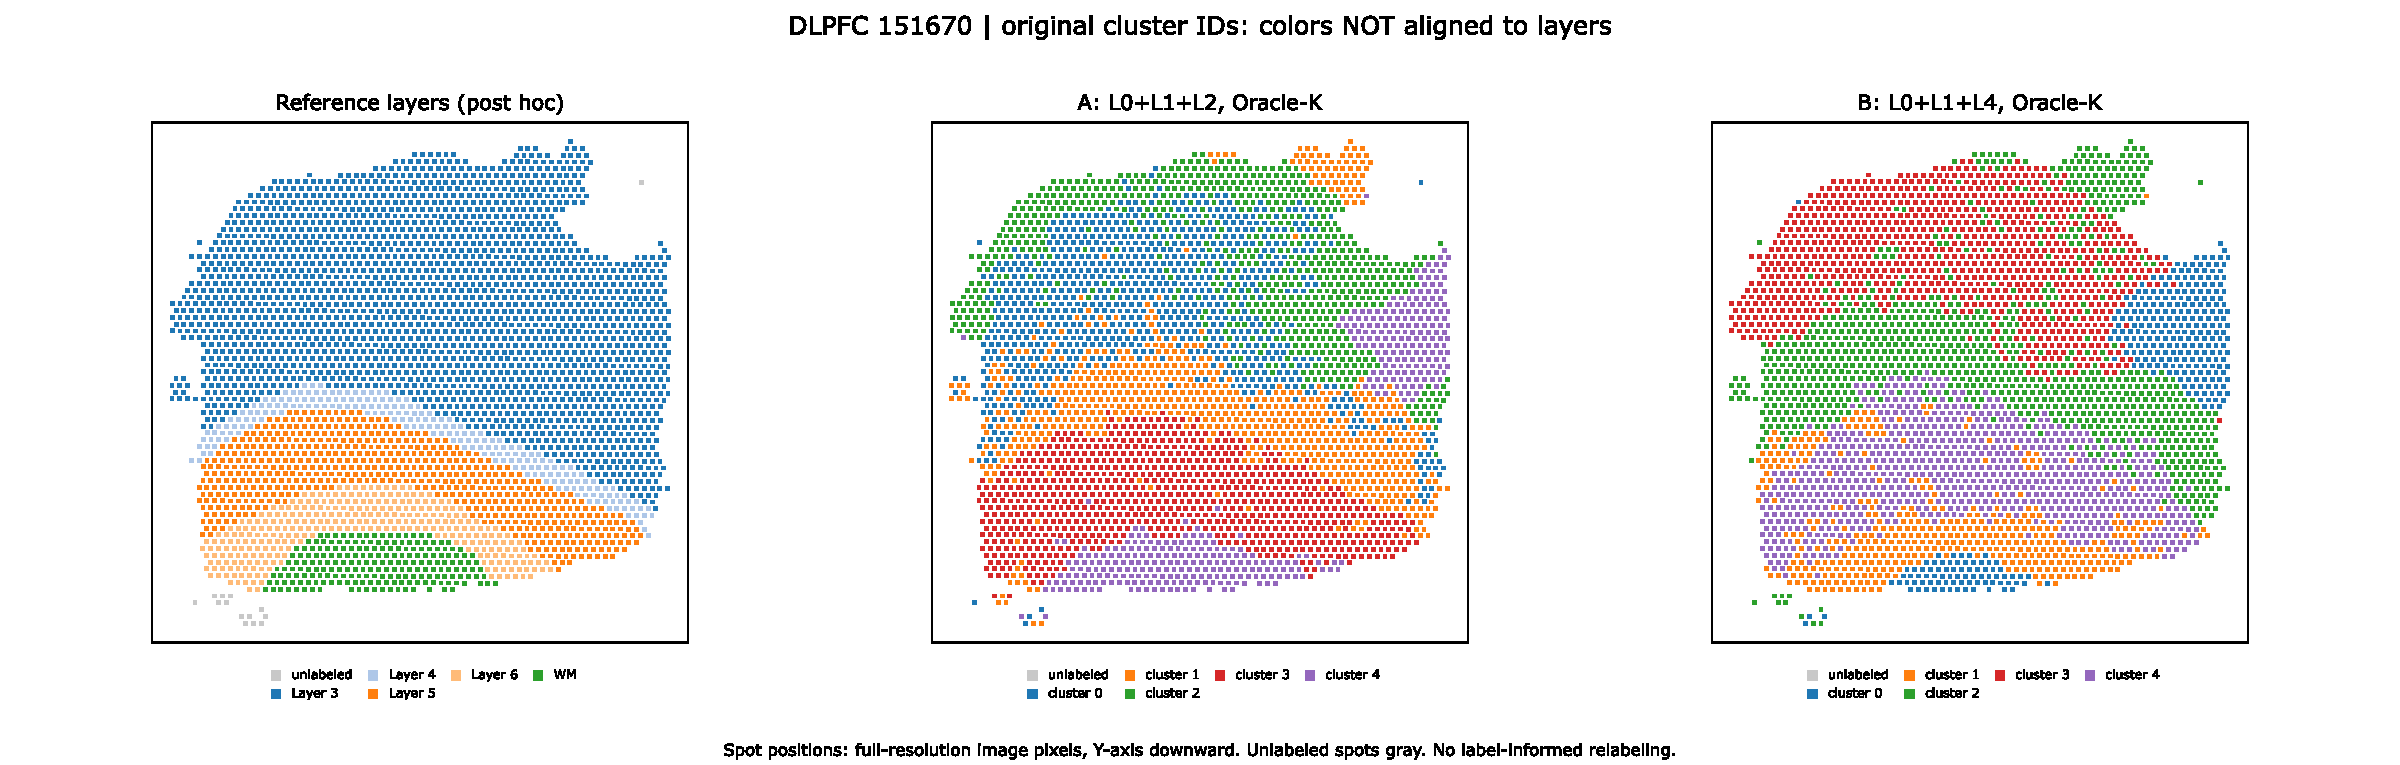
\includegraphics[width=0.97\linewidth,height=0.72\textheight,keepaspectratio]{E4_SOURCE_FIGURES_20261122_RELEASE/figures_pdf/151670/151670_reference_A_B_spatial.pdf}
\captionof{figure}{DLPFC切片151670：参考层与A/B原始聚类三联图（原始E4图件转换的矢量PDF；聚类编号未根据参考标签重排）。}
\label{fig:cc-e4-app-151670-map}
\end{minipage}\par\medskip
}{%
\par\noindent\emph{[编译提示：未找到该图件的PDF，请检查相对路径。]}\par
}
\IfFileExists{E4_SOURCE_FIGURES_20261122_RELEASE/figures_pdf/151670/151670_MOBP_PCP4_SNAP25_expression.pdf}{%
\par\noindent\begin{minipage}{\linewidth}
\centering
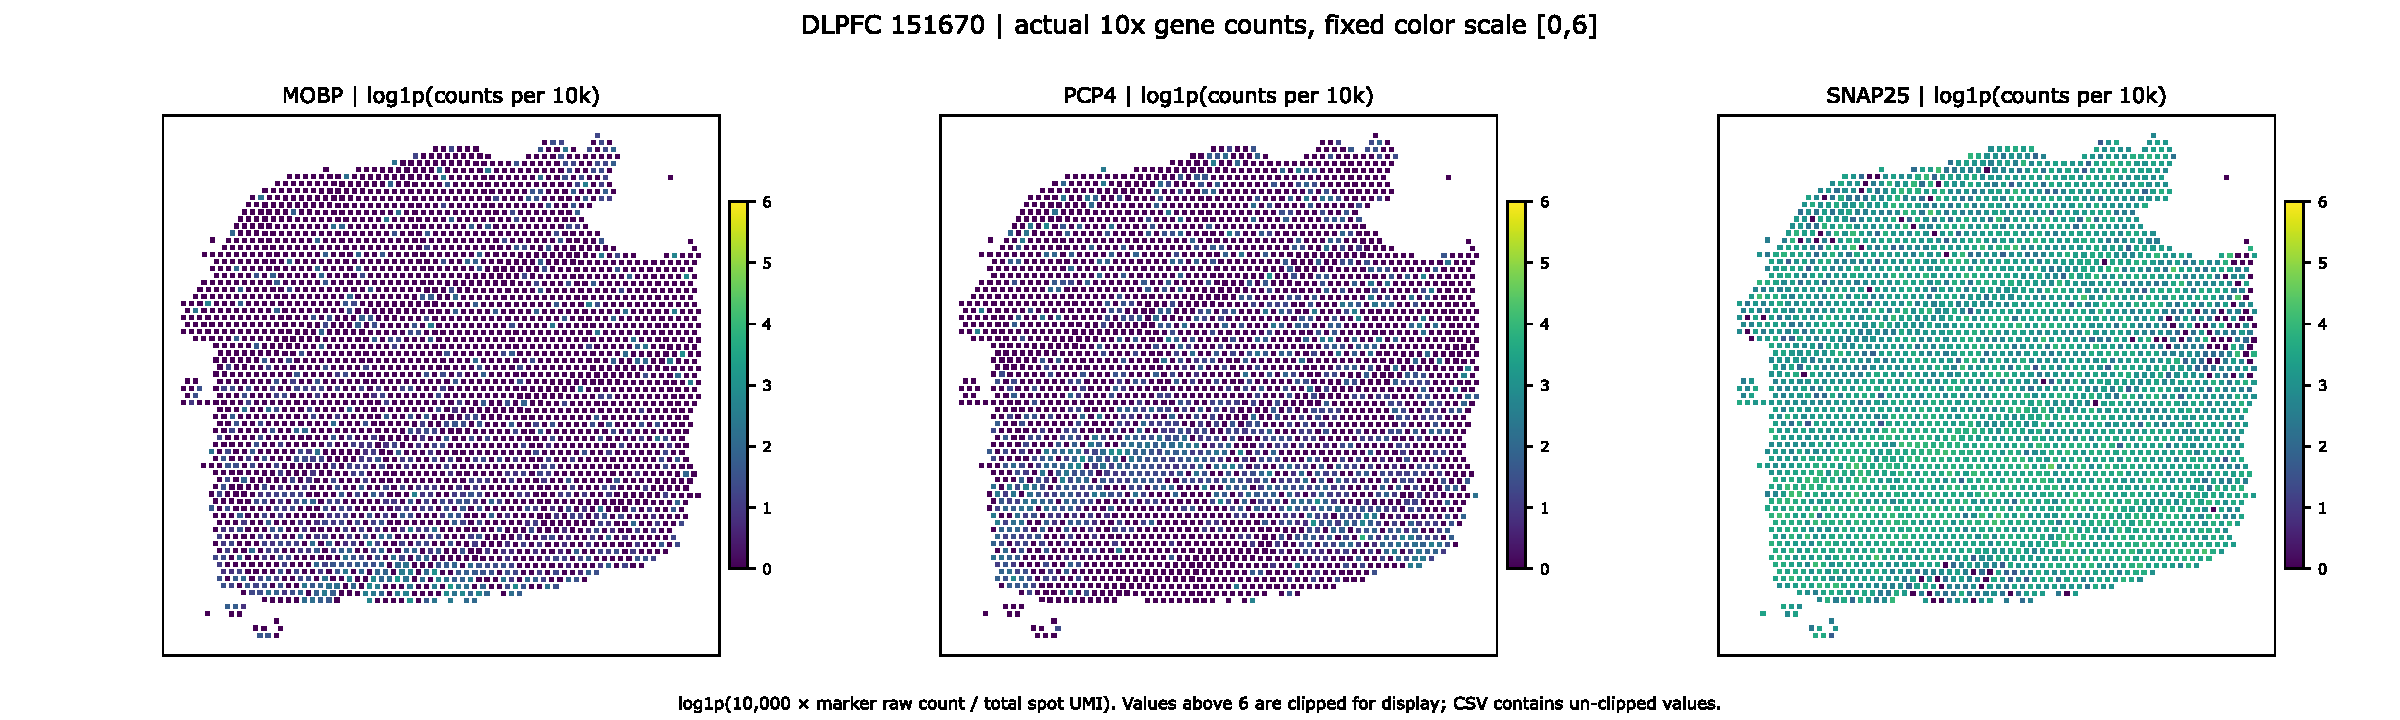
\includegraphics[width=0.97\linewidth,height=0.72\textheight,keepaspectratio]{E4_SOURCE_FIGURES_20261122_RELEASE/figures_pdf/151670/151670_MOBP_PCP4_SNAP25_expression.pdf}
\captionof{figure}{DLPFC切片151670：MOBP/PCP4/SNAP25表达三联图（原始E4图件转换的矢量PDF；聚类编号未根据参考标签重排）。}
\label{fig:cc-e4-app-151670-markers}
\end{minipage}\par\medskip
}{%
\par\noindent\emph{[编译提示：未找到该图件的PDF，请检查相对路径。]}\par
}
\IfFileExists{E4_SOURCE_FIGURES_20261122_RELEASE/figures_pdf/151670/151670_reference_A_B_confusion.pdf}{%
\par\noindent\begin{minipage}{\linewidth}
\centering
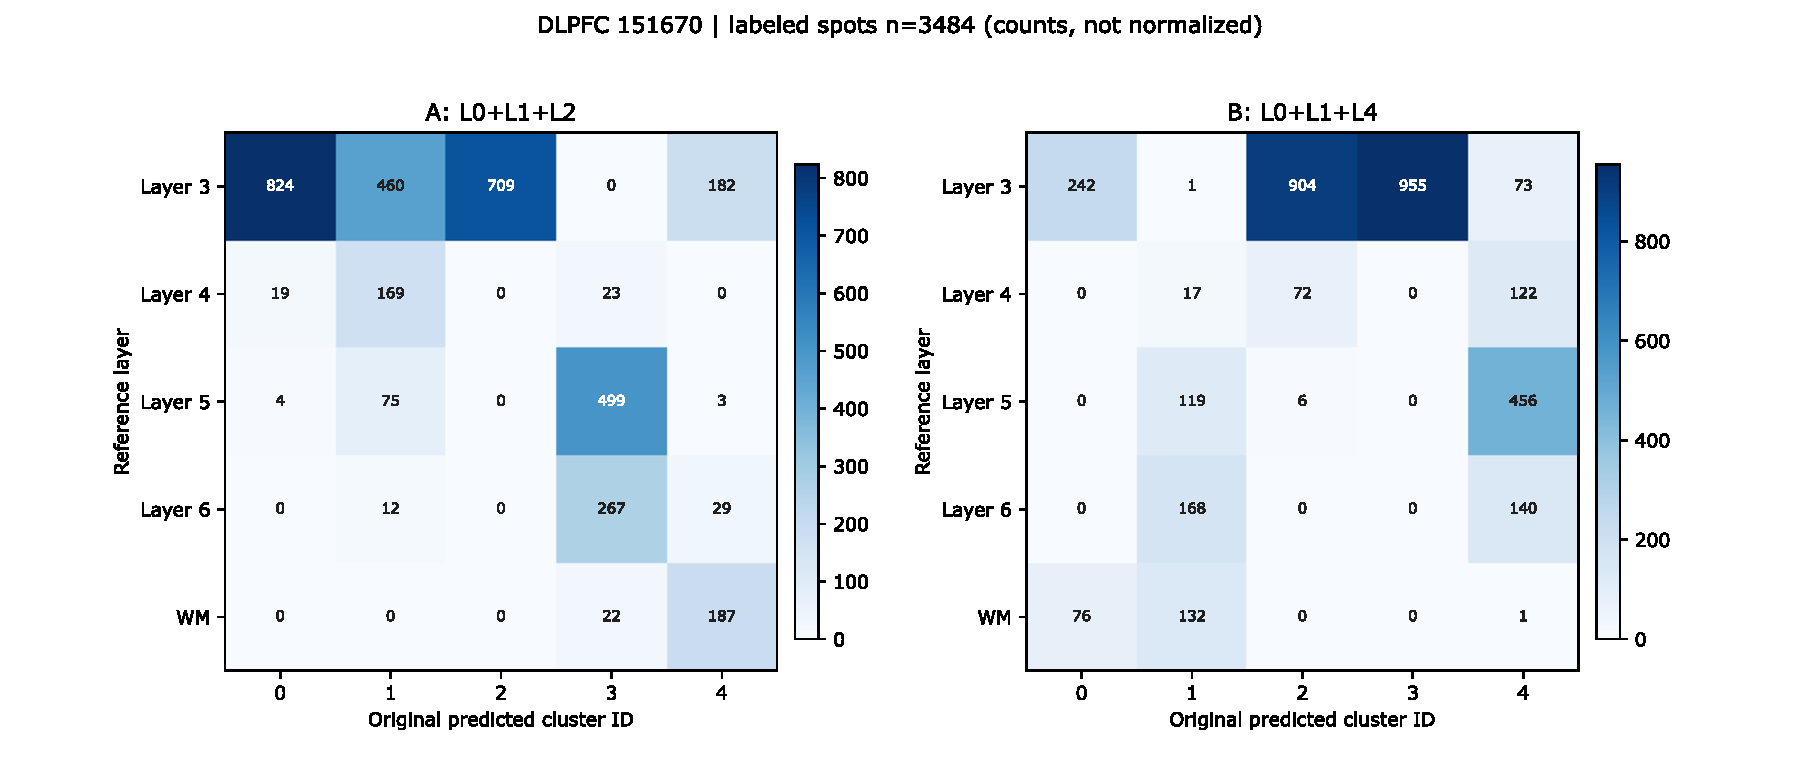
\includegraphics[width=0.97\linewidth,height=0.72\textheight,keepaspectratio]{E4_SOURCE_FIGURES_20261122_RELEASE/figures_pdf/151670/151670_reference_A_B_confusion.pdf}
\captionof{figure}{DLPFC切片151670：参考层与A/B簇交叉计数图（原始E4图件转换的矢量PDF；聚类编号未根据参考标签重排）。}
\label{fig:cc-e4-app-151670-confusion}
\end{minipage}\par\medskip
}{%
\par\noindent\emph{[编译提示：未找到该图件的PDF，请检查相对路径。]}\par
}
\subsection{DLPFC切片151671}
\IfFileExists{E4_SOURCE_FIGURES_20261122_RELEASE/figures_pdf/151671/151671_reference_A_B_spatial.pdf}{%
\par\noindent\begin{minipage}{\linewidth}
\centering
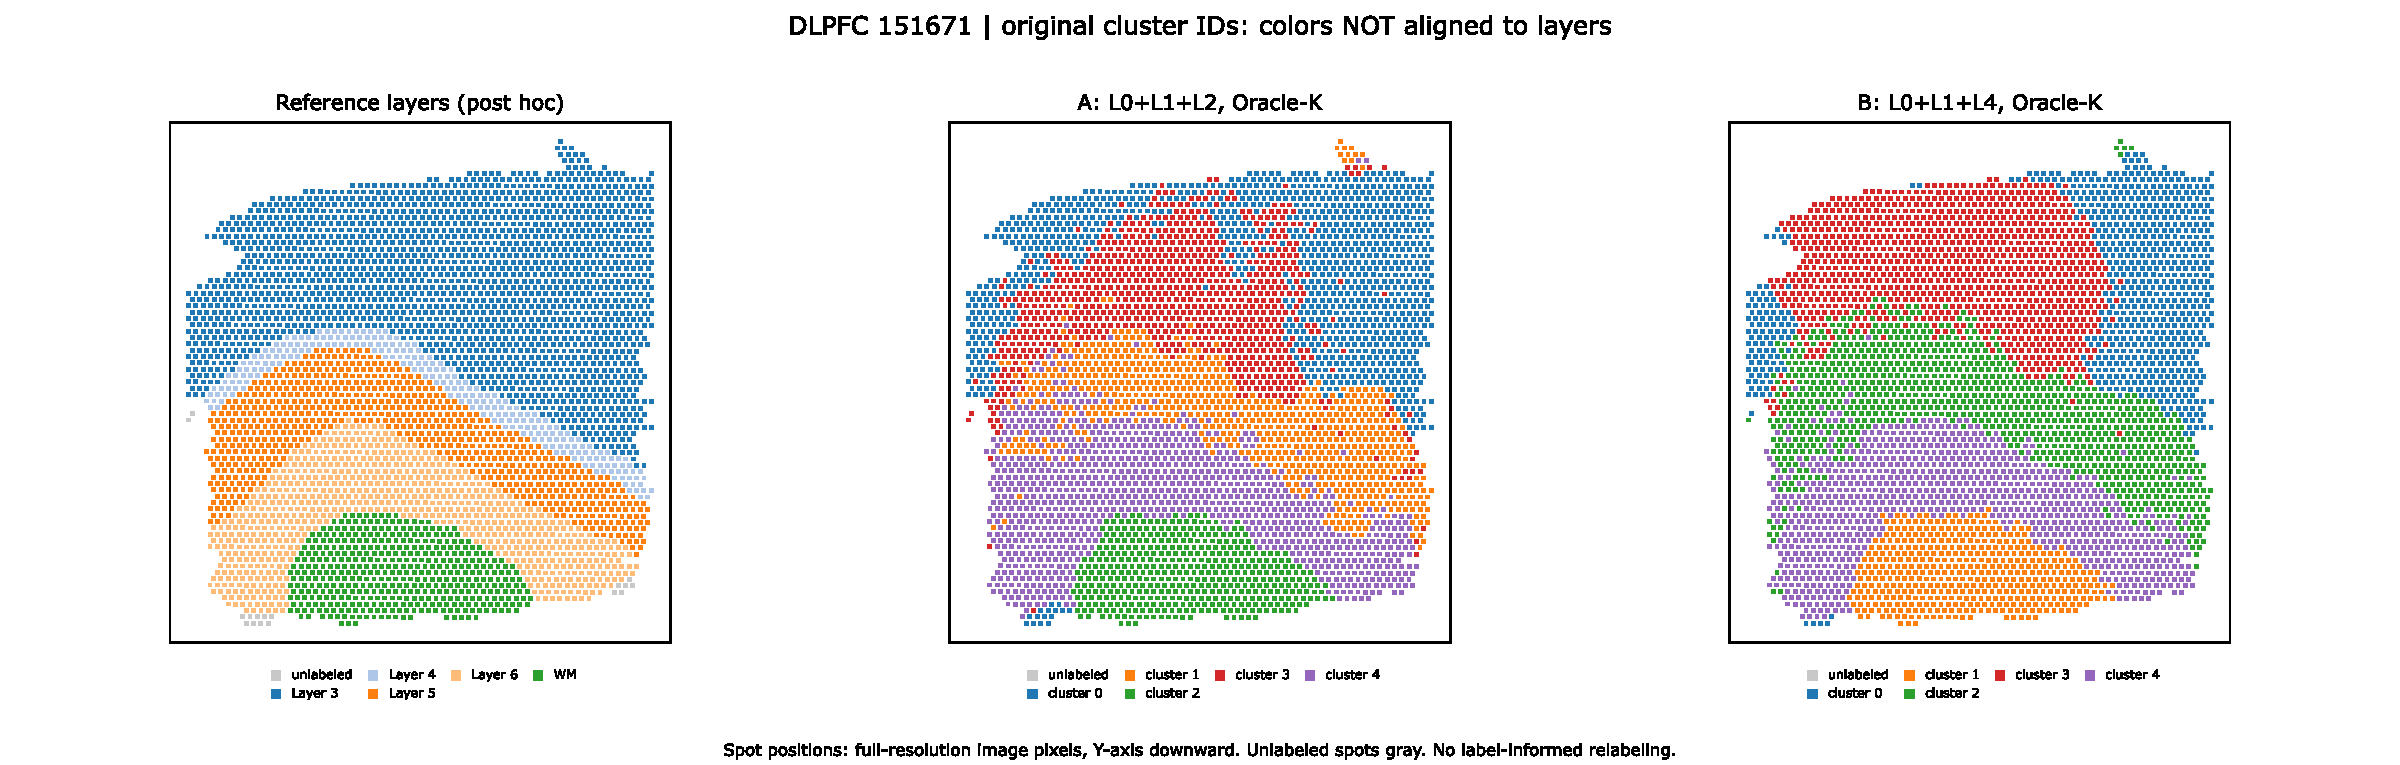
\includegraphics[width=0.97\linewidth,height=0.72\textheight,keepaspectratio]{E4_SOURCE_FIGURES_20261122_RELEASE/figures_pdf/151671/151671_reference_A_B_spatial.pdf}
\captionof{figure}{DLPFC切片151671：参考层与A/B原始聚类三联图（原始E4图件转换的矢量PDF；聚类编号未根据参考标签重排）。}
\label{fig:cc-e4-app-151671-map}
\end{minipage}\par\medskip
}{%
\par\noindent\emph{[编译提示：未找到该图件的PDF，请检查相对路径。]}\par
}
\IfFileExists{E4_SOURCE_FIGURES_20261122_RELEASE/figures_pdf/151671/151671_MOBP_PCP4_SNAP25_expression.pdf}{%
\par\noindent\begin{minipage}{\linewidth}
\centering
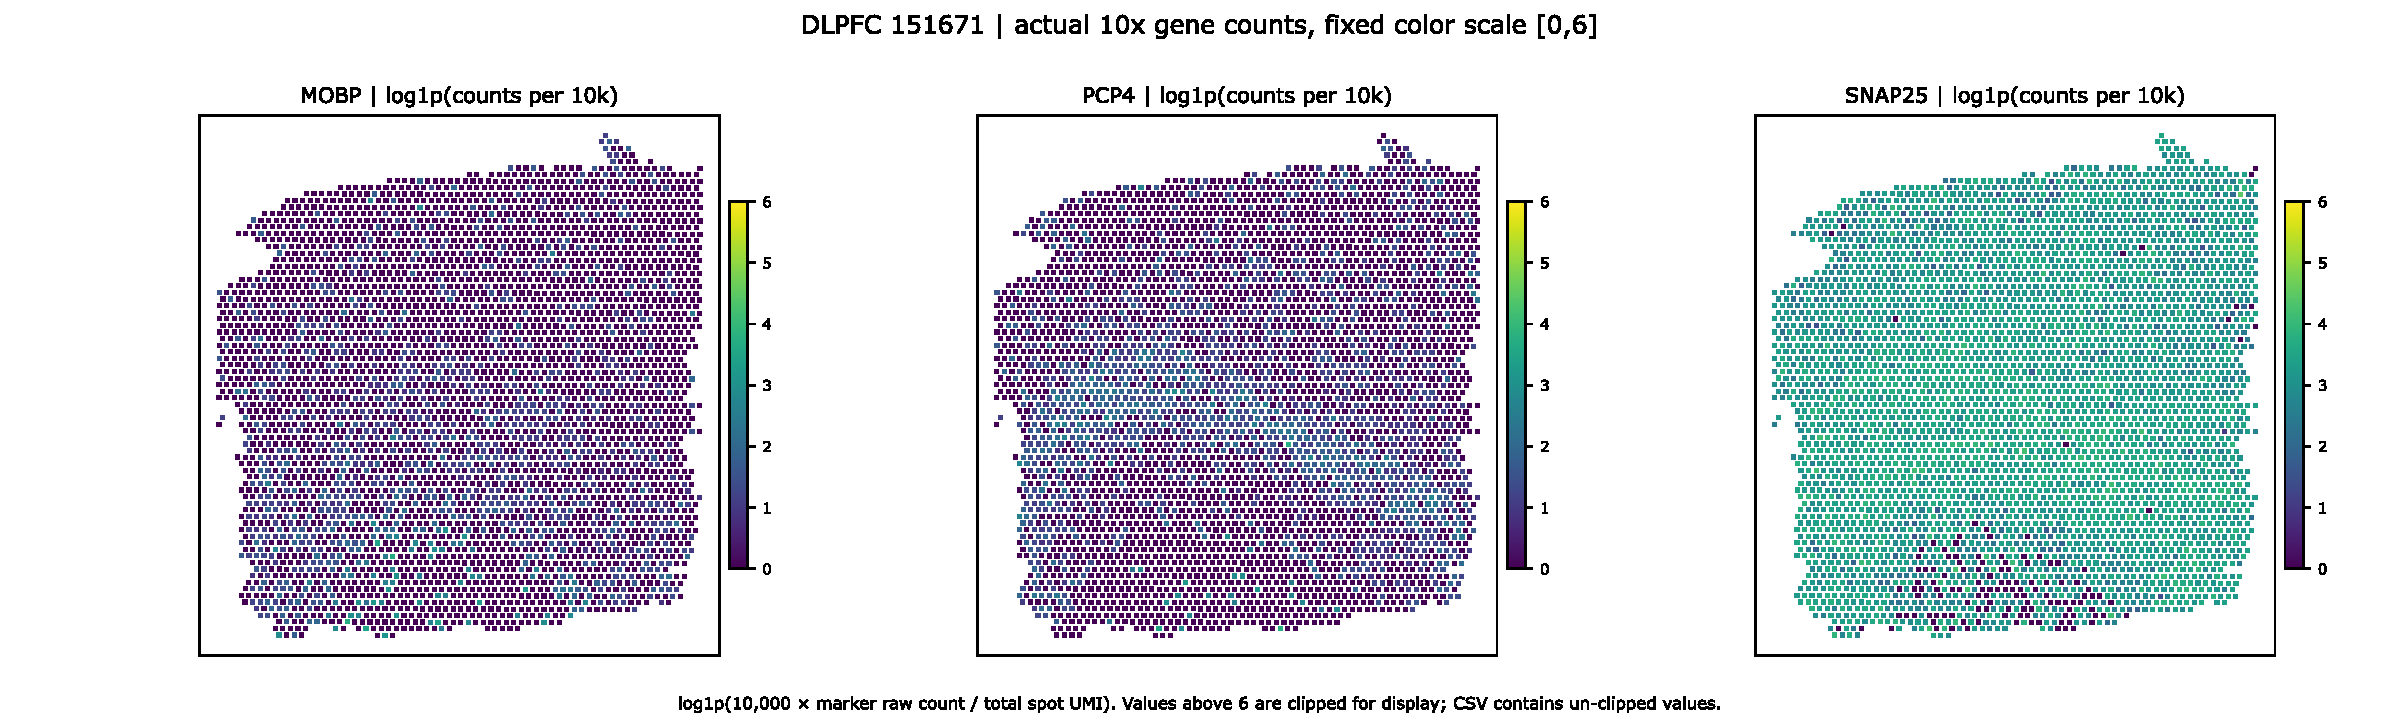
\includegraphics[width=0.97\linewidth,height=0.72\textheight,keepaspectratio]{E4_SOURCE_FIGURES_20261122_RELEASE/figures_pdf/151671/151671_MOBP_PCP4_SNAP25_expression.pdf}
\captionof{figure}{DLPFC切片151671：MOBP/PCP4/SNAP25表达三联图（原始E4图件转换的矢量PDF；聚类编号未根据参考标签重排）。}
\label{fig:cc-e4-app-151671-markers}
\end{minipage}\par\medskip
}{%
\par\noindent\emph{[编译提示：未找到该图件的PDF，请检查相对路径。]}\par
}
\IfFileExists{E4_SOURCE_FIGURES_20261122_RELEASE/figures_pdf/151671/151671_reference_A_B_confusion.pdf}{%
\par\noindent\begin{minipage}{\linewidth}
\centering
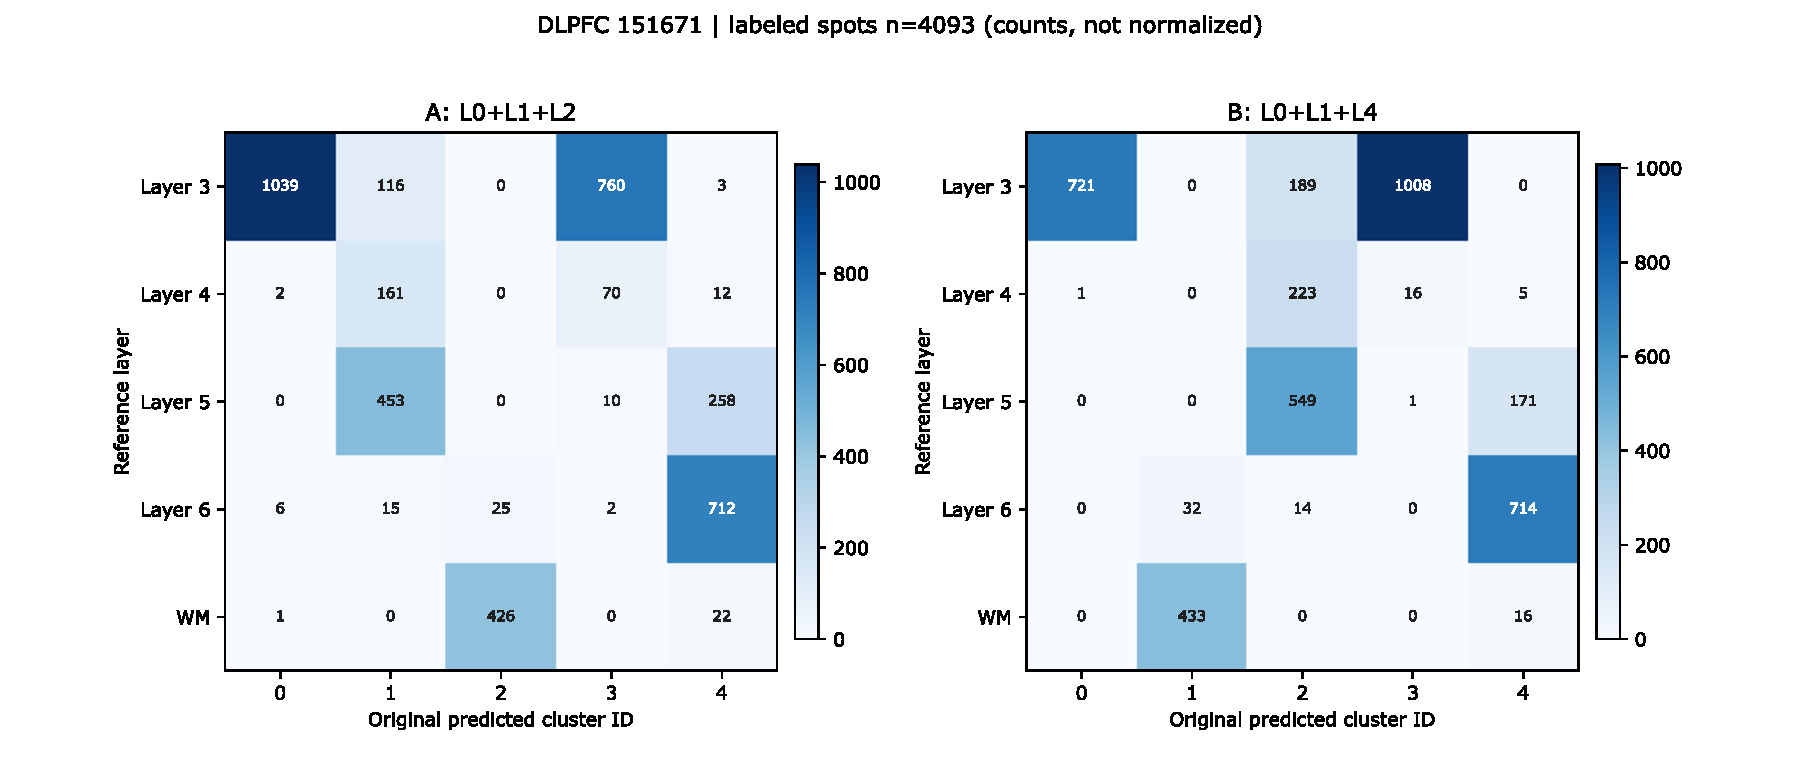
\includegraphics[width=0.97\linewidth,height=0.72\textheight,keepaspectratio]{E4_SOURCE_FIGURES_20261122_RELEASE/figures_pdf/151671/151671_reference_A_B_confusion.pdf}
\captionof{figure}{DLPFC切片151671：参考层与A/B簇交叉计数图（原始E4图件转换的矢量PDF；聚类编号未根据参考标签重排）。}
\label{fig:cc-e4-app-151671-confusion}
\end{minipage}\par\medskip
}{%
\par\noindent\emph{[编译提示：未找到该图件的PDF，请检查相对路径。]}\par
}
\subsection{DLPFC切片151672}
\IfFileExists{E4_SOURCE_FIGURES_20261122_RELEASE/figures_pdf/151672/151672_reference_A_B_spatial.pdf}{%
\par\noindent\begin{minipage}{\linewidth}
\centering
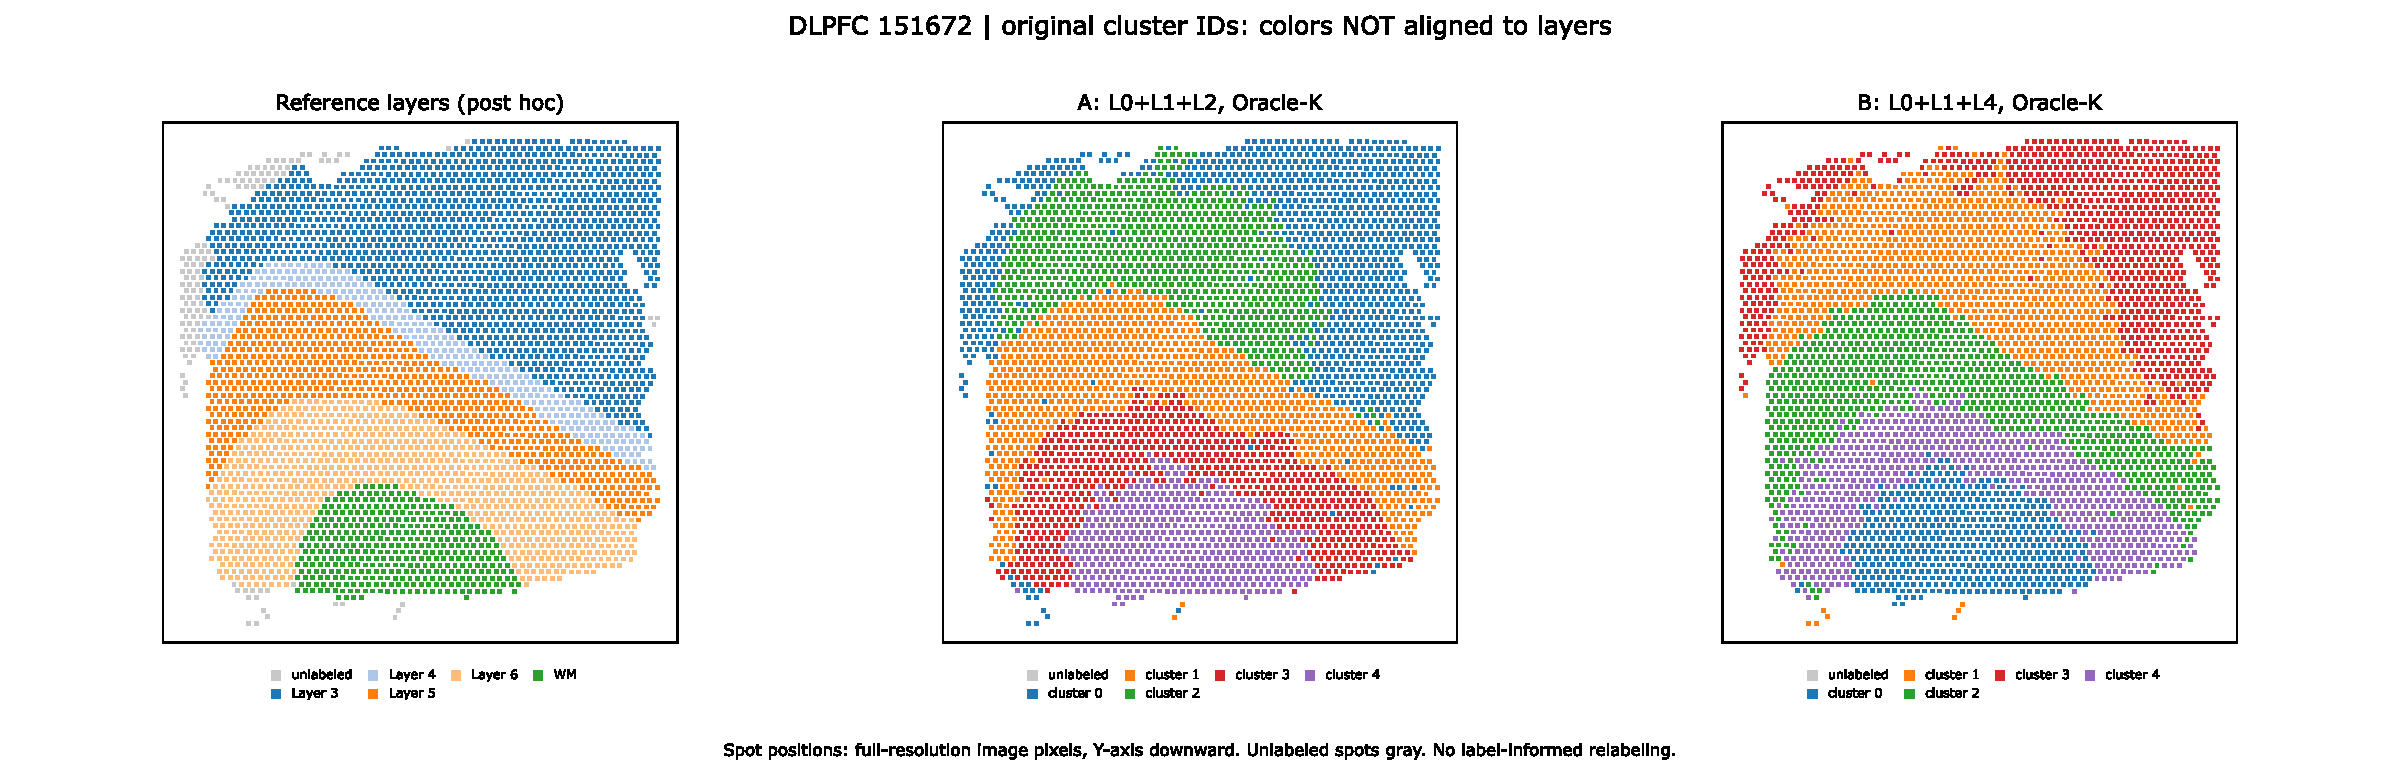
\includegraphics[width=0.97\linewidth,height=0.72\textheight,keepaspectratio]{E4_SOURCE_FIGURES_20261122_RELEASE/figures_pdf/151672/151672_reference_A_B_spatial.pdf}
\captionof{figure}{DLPFC切片151672：参考层与A/B原始聚类三联图（原始E4图件转换的矢量PDF；聚类编号未根据参考标签重排）。}
\label{fig:cc-e4-app-151672-map}
\end{minipage}\par\medskip
}{%
\par\noindent\emph{[编译提示：未找到该图件的PDF，请检查相对路径。]}\par
}
\IfFileExists{E4_SOURCE_FIGURES_20261122_RELEASE/figures_pdf/151672/151672_MOBP_PCP4_SNAP25_expression.pdf}{%
\par\noindent\begin{minipage}{\linewidth}
\centering
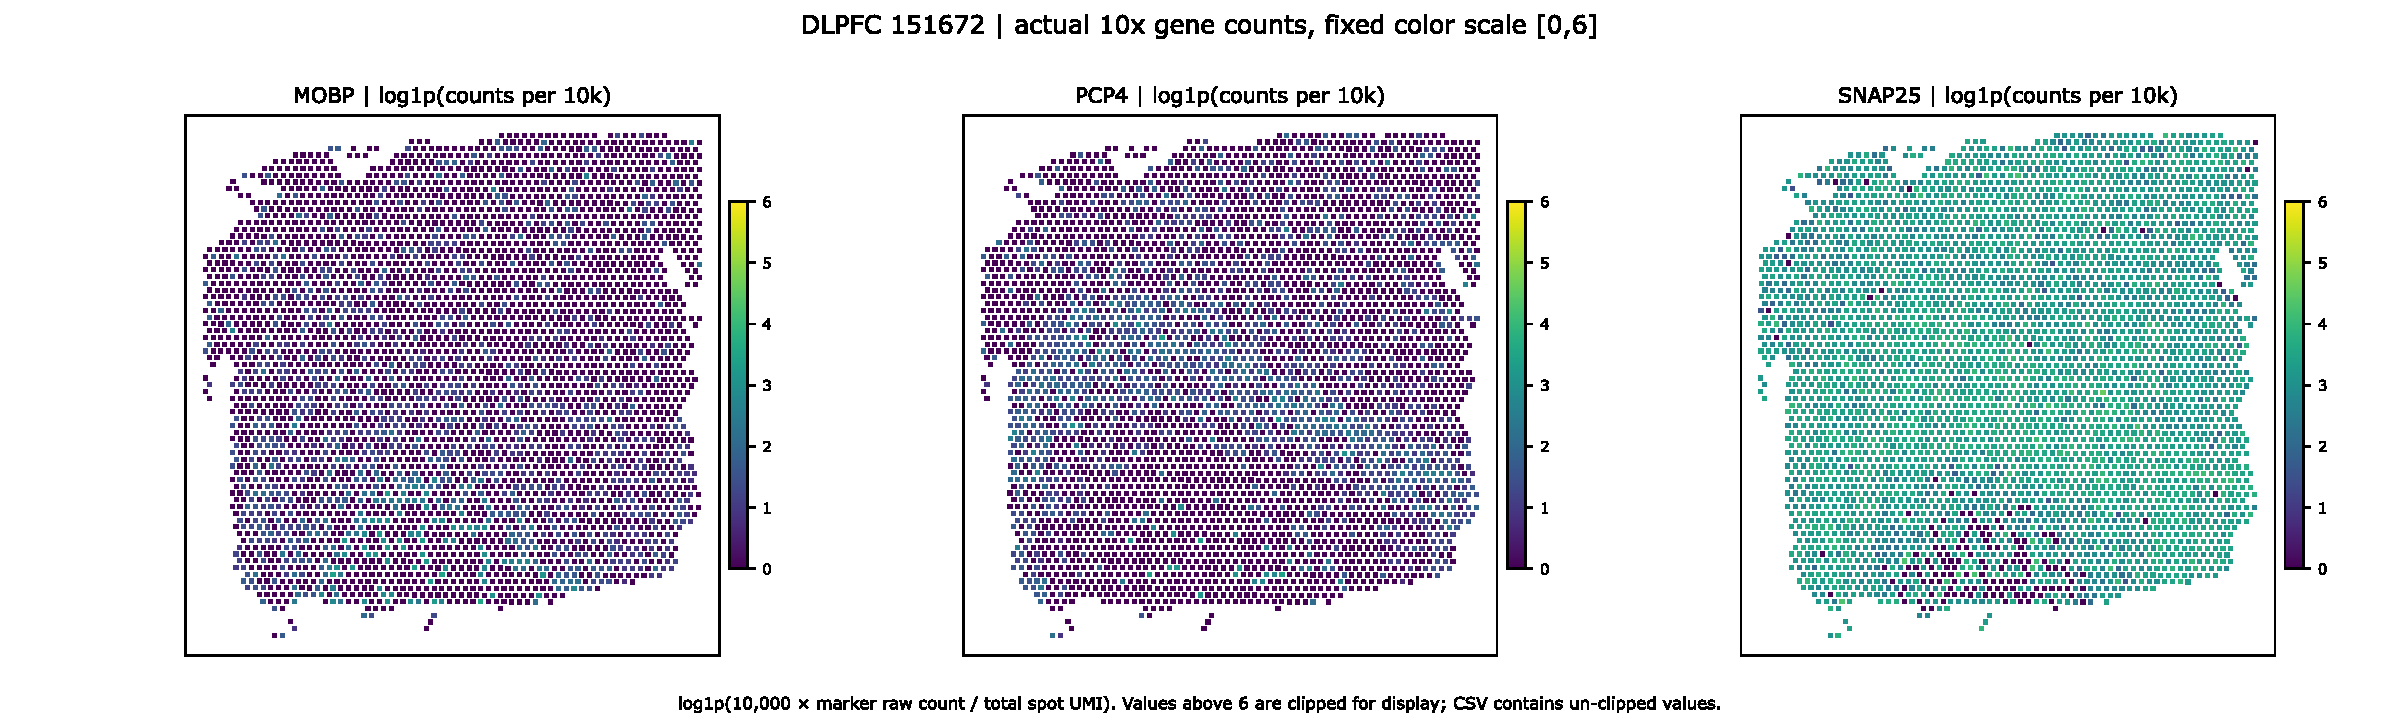
\includegraphics[width=0.97\linewidth,height=0.72\textheight,keepaspectratio]{E4_SOURCE_FIGURES_20261122_RELEASE/figures_pdf/151672/151672_MOBP_PCP4_SNAP25_expression.pdf}
\captionof{figure}{DLPFC切片151672：MOBP/PCP4/SNAP25表达三联图（原始E4图件转换的矢量PDF；聚类编号未根据参考标签重排）。}
\label{fig:cc-e4-app-151672-markers}
\end{minipage}\par\medskip
}{%
\par\noindent\emph{[编译提示：未找到该图件的PDF，请检查相对路径。]}\par
}
\IfFileExists{E4_SOURCE_FIGURES_20261122_RELEASE/figures_pdf/151672/151672_reference_A_B_confusion.pdf}{%
\par\noindent\begin{minipage}{\linewidth}
\centering
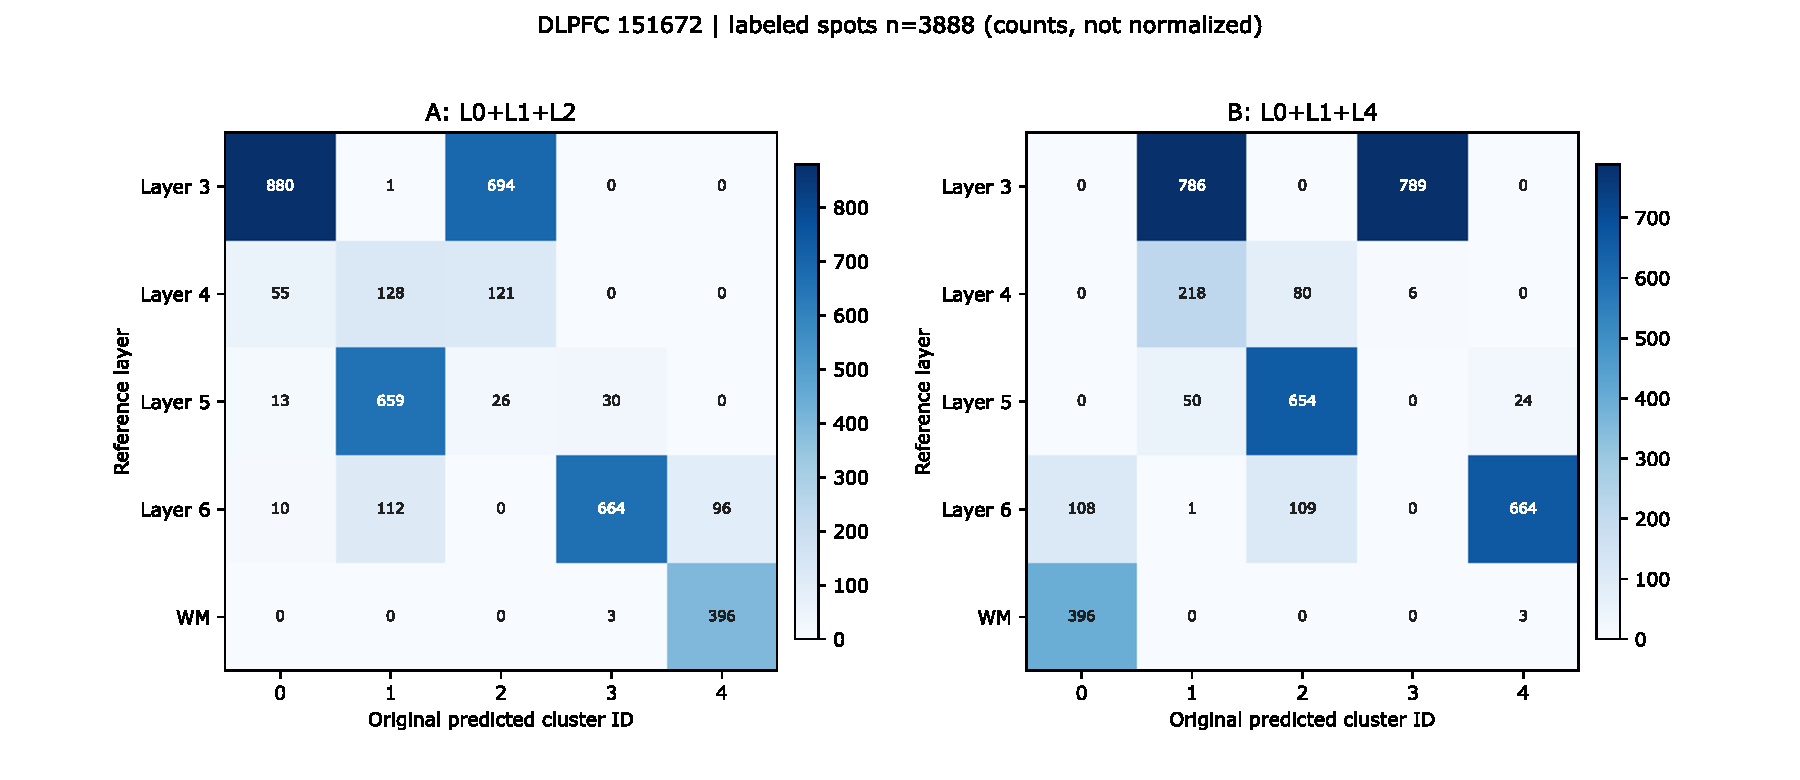
\includegraphics[width=0.97\linewidth,height=0.72\textheight,keepaspectratio]{E4_SOURCE_FIGURES_20261122_RELEASE/figures_pdf/151672/151672_reference_A_B_confusion.pdf}
\captionof{figure}{DLPFC切片151672：参考层与A/B簇交叉计数图（原始E4图件转换的矢量PDF；聚类编号未根据参考标签重排）。}
\label{fig:cc-e4-app-151672-confusion}
\end{minipage}\par\medskip
}{%
\par\noindent\emph{[编译提示：未找到该图件的PDF，请检查相对路径。]}\par
}
\subsection{DLPFC切片151673}
\IfFileExists{E4_SOURCE_FIGURES_20261122_RELEASE/figures_pdf/151673/151673_reference_A_B_spatial.pdf}{%
\par\noindent\begin{minipage}{\linewidth}
\centering
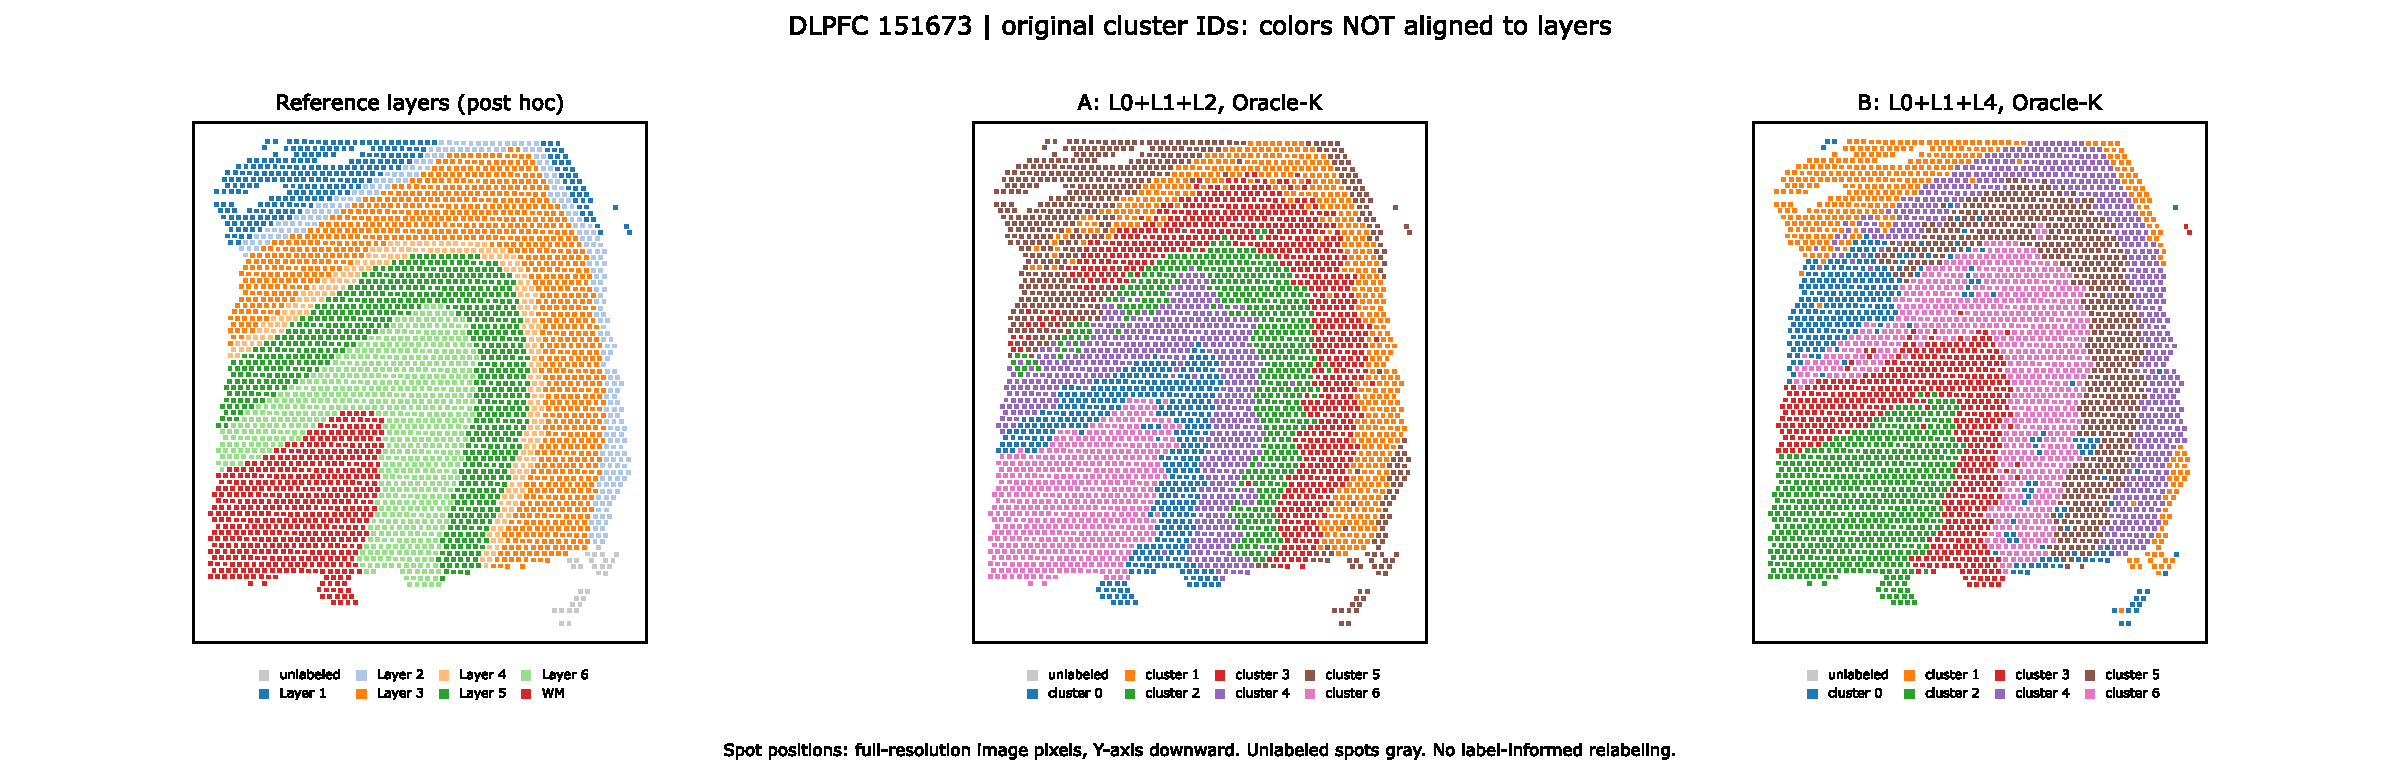
\includegraphics[width=0.97\linewidth,height=0.72\textheight,keepaspectratio]{E4_SOURCE_FIGURES_20261122_RELEASE/figures_pdf/151673/151673_reference_A_B_spatial.pdf}
\captionof{figure}{DLPFC切片151673：参考层与A/B原始聚类三联图（原始E4图件转换的矢量PDF；聚类编号未根据参考标签重排）。}
\label{fig:cc-e4-app-151673-map}
\end{minipage}\par\medskip
}{%
\par\noindent\emph{[编译提示：未找到该图件的PDF，请检查相对路径。]}\par
}
\IfFileExists{E4_SOURCE_FIGURES_20261122_RELEASE/figures_pdf/151673/151673_MOBP_PCP4_SNAP25_expression.pdf}{%
\par\noindent\begin{minipage}{\linewidth}
\centering
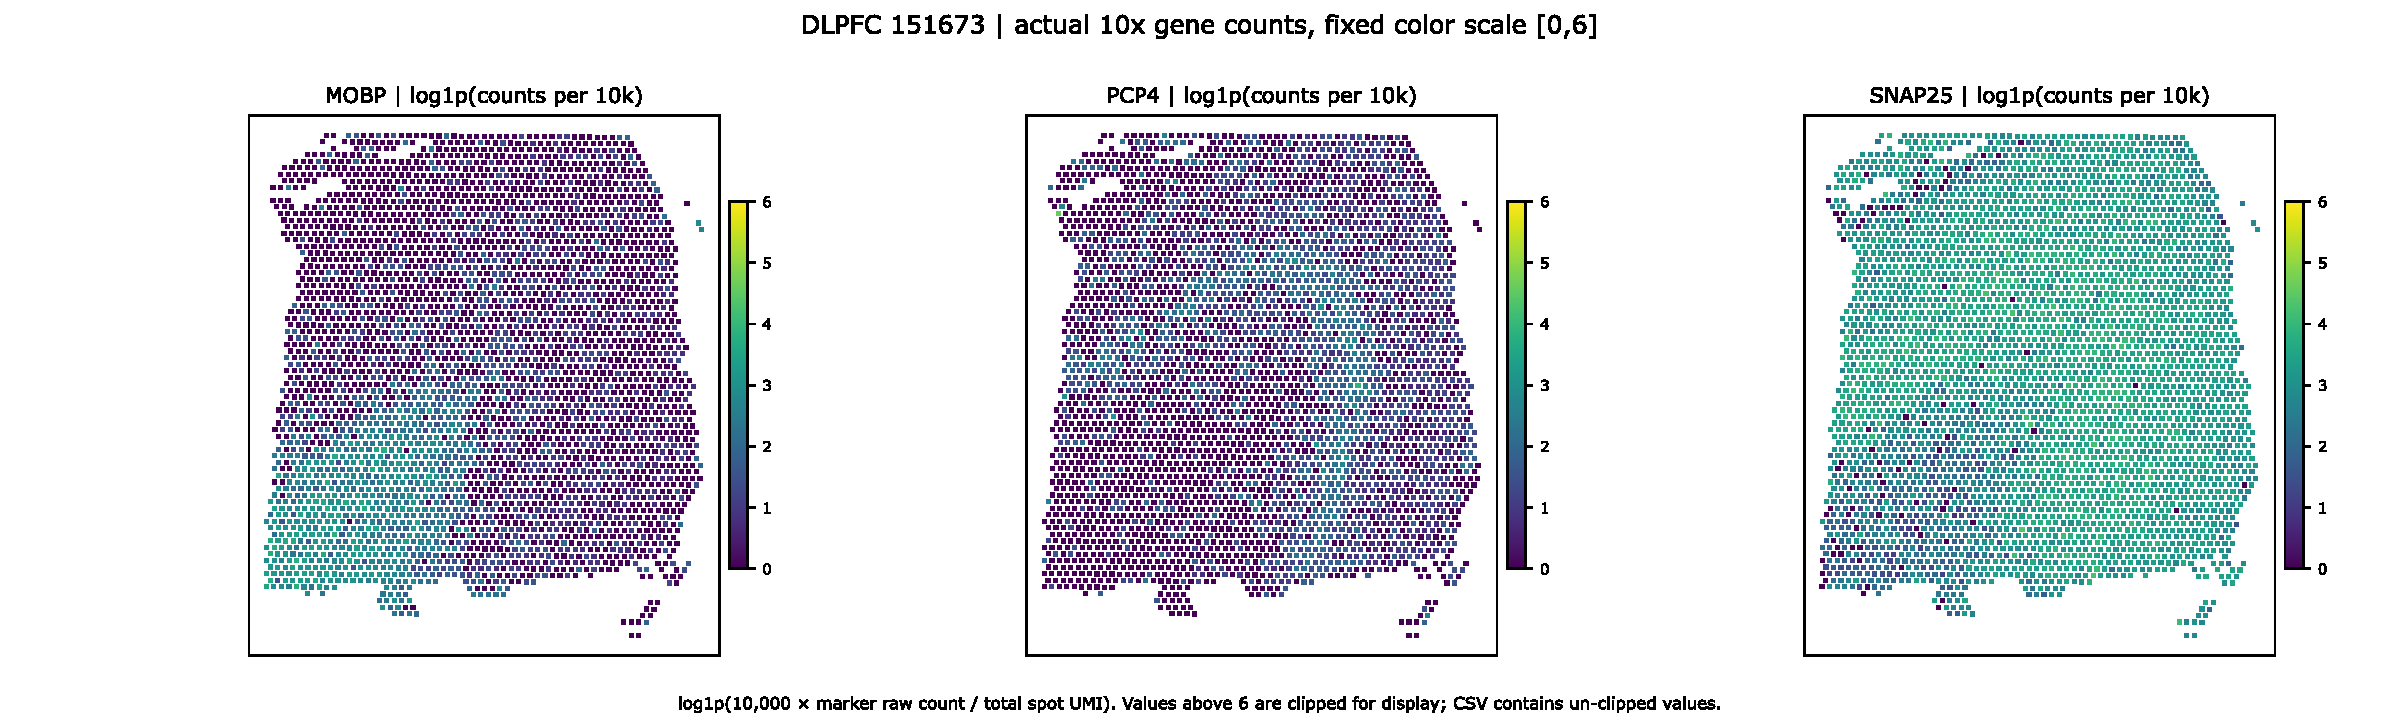
\includegraphics[width=0.97\linewidth,height=0.72\textheight,keepaspectratio]{E4_SOURCE_FIGURES_20261122_RELEASE/figures_pdf/151673/151673_MOBP_PCP4_SNAP25_expression.pdf}
\captionof{figure}{DLPFC切片151673：MOBP/PCP4/SNAP25表达三联图（原始E4图件转换的矢量PDF；聚类编号未根据参考标签重排）。}
\label{fig:cc-e4-app-151673-markers}
\end{minipage}\par\medskip
}{%
\par\noindent\emph{[编译提示：未找到该图件的PDF，请检查相对路径。]}\par
}
\IfFileExists{E4_SOURCE_FIGURES_20261122_RELEASE/figures_pdf/151673/151673_reference_A_B_confusion.pdf}{%
\par\noindent\begin{minipage}{\linewidth}
\centering
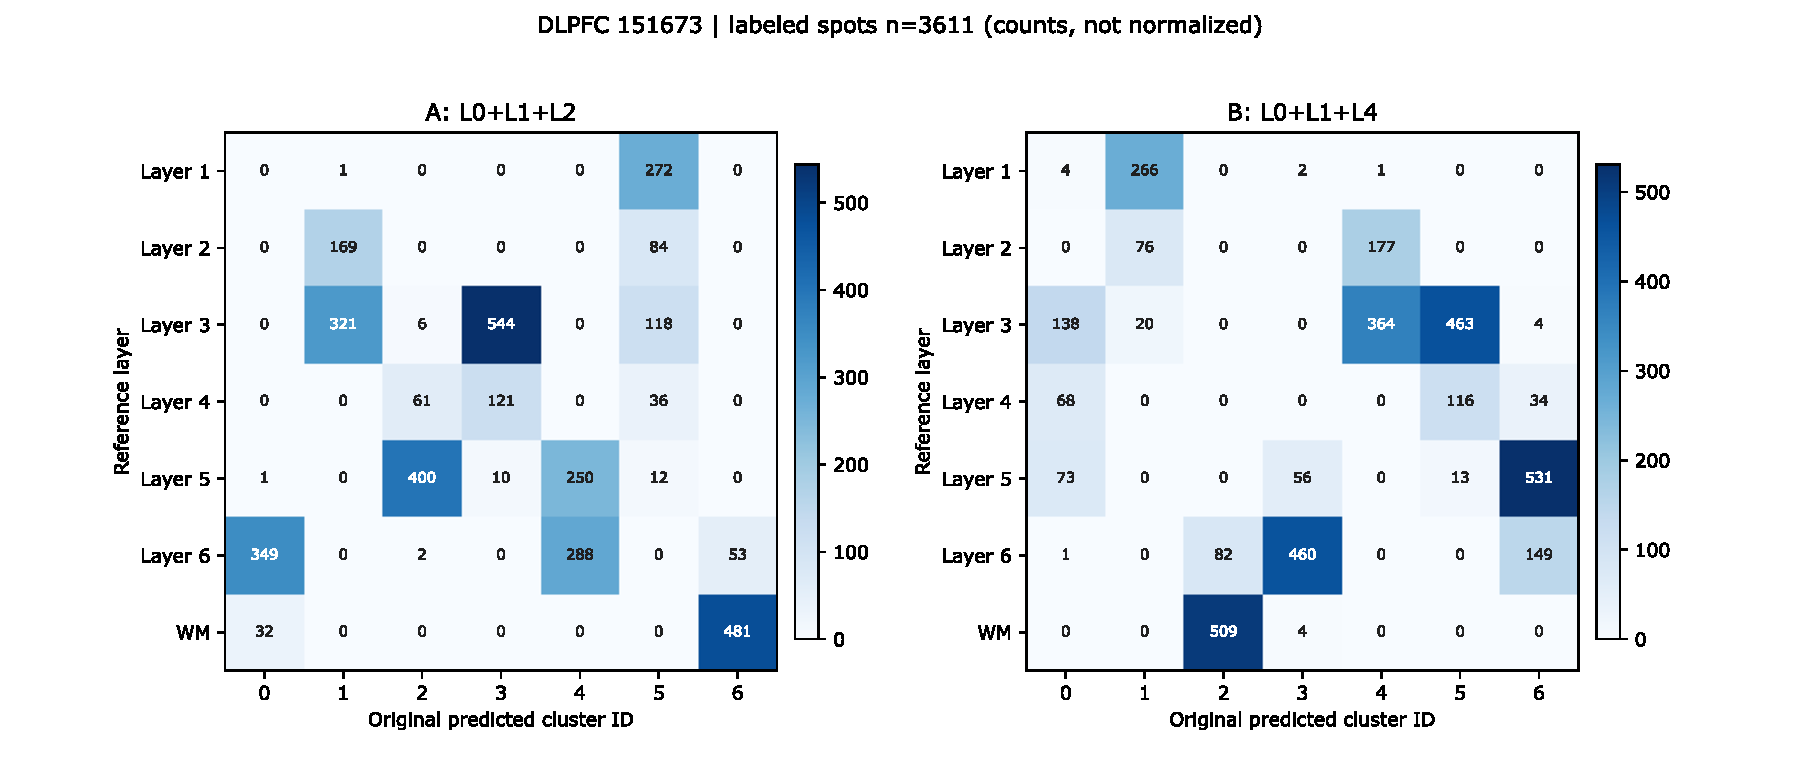
\includegraphics[width=0.97\linewidth,height=0.72\textheight,keepaspectratio]{E4_SOURCE_FIGURES_20261122_RELEASE/figures_pdf/151673/151673_reference_A_B_confusion.pdf}
\captionof{figure}{DLPFC切片151673：参考层与A/B簇交叉计数图（原始E4图件转换的矢量PDF；聚类编号未根据参考标签重排）。}
\label{fig:cc-e4-app-151673-confusion}
\end{minipage}\par\medskip
}{%
\par\noindent\emph{[编译提示：未找到该图件的PDF，请检查相对路径。]}\par
}
\subsection{DLPFC切片151674}
\IfFileExists{E4_SOURCE_FIGURES_20261122_RELEASE/figures_pdf/151674/151674_reference_A_B_spatial.pdf}{%
\par\noindent\begin{minipage}{\linewidth}
\centering
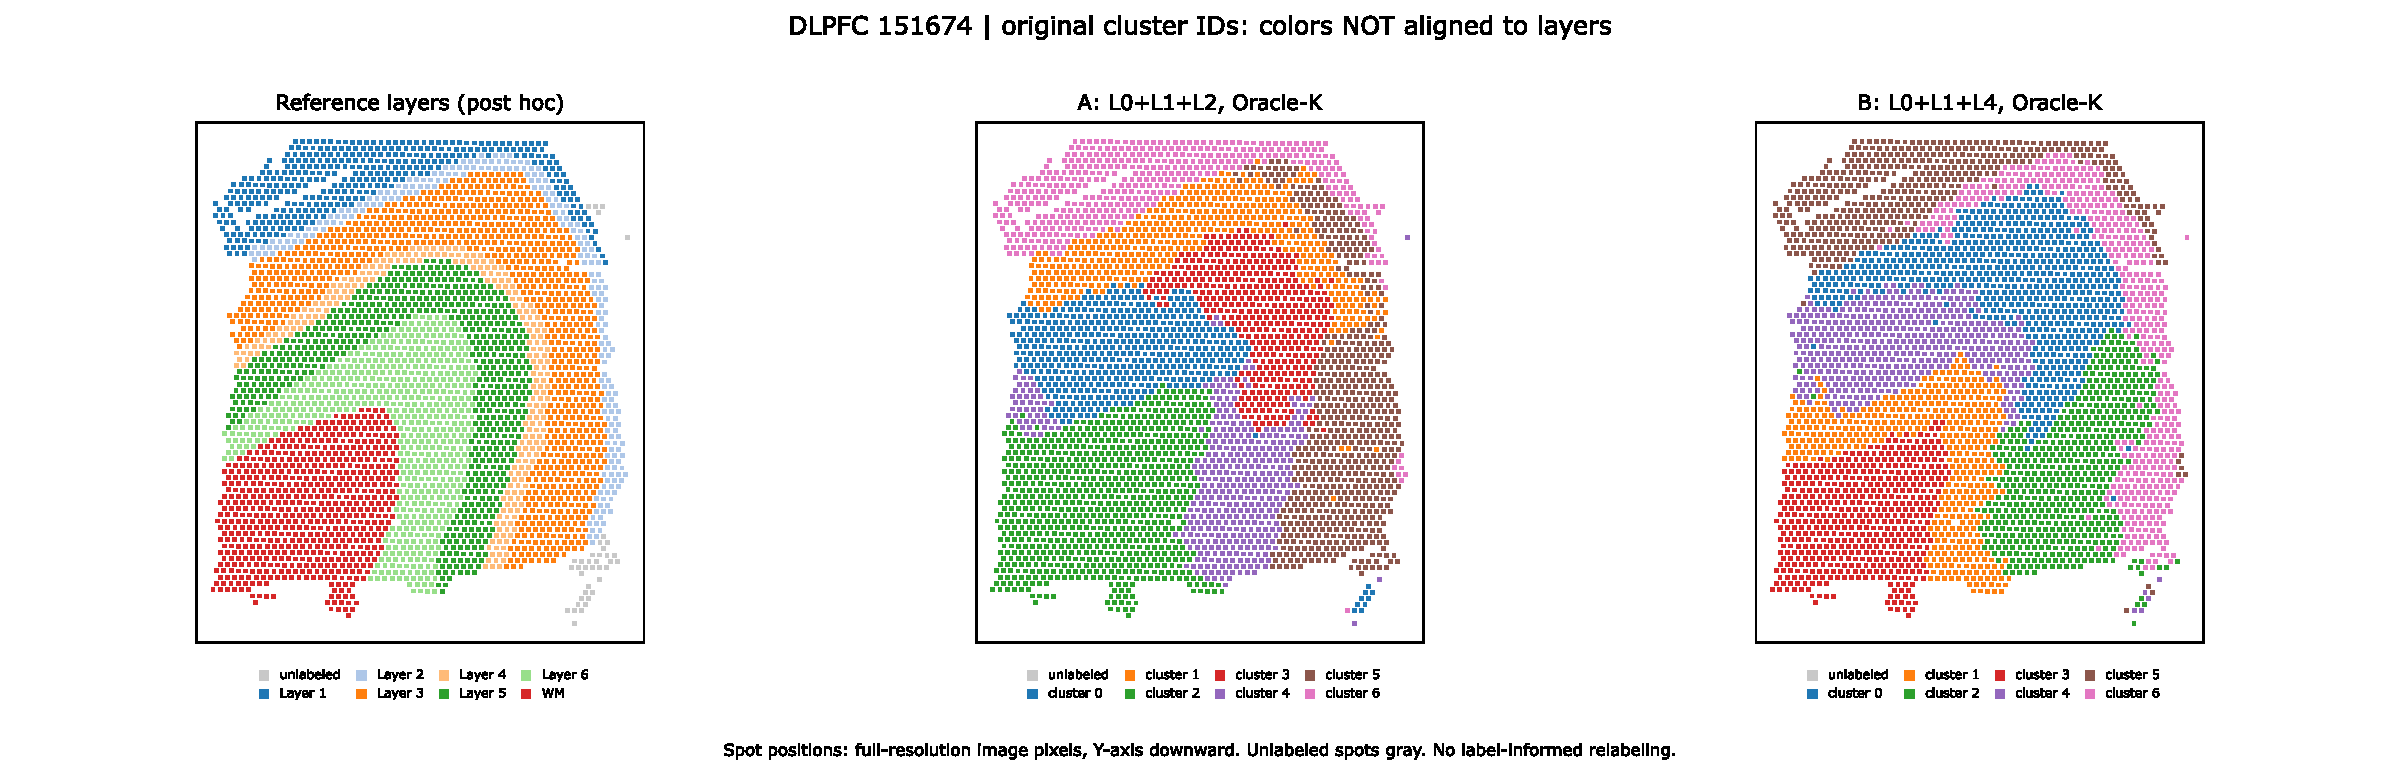
\includegraphics[width=0.97\linewidth,height=0.72\textheight,keepaspectratio]{E4_SOURCE_FIGURES_20261122_RELEASE/figures_pdf/151674/151674_reference_A_B_spatial.pdf}
\captionof{figure}{DLPFC切片151674：参考层与A/B原始聚类三联图（原始E4图件转换的矢量PDF；聚类编号未根据参考标签重排）。}
\label{fig:cc-e4-app-151674-map}
\end{minipage}\par\medskip
}{%
\par\noindent\emph{[编译提示：未找到该图件的PDF，请检查相对路径。]}\par
}
\IfFileExists{E4_SOURCE_FIGURES_20261122_RELEASE/figures_pdf/151674/151674_MOBP_PCP4_SNAP25_expression.pdf}{%
\par\noindent\begin{minipage}{\linewidth}
\centering
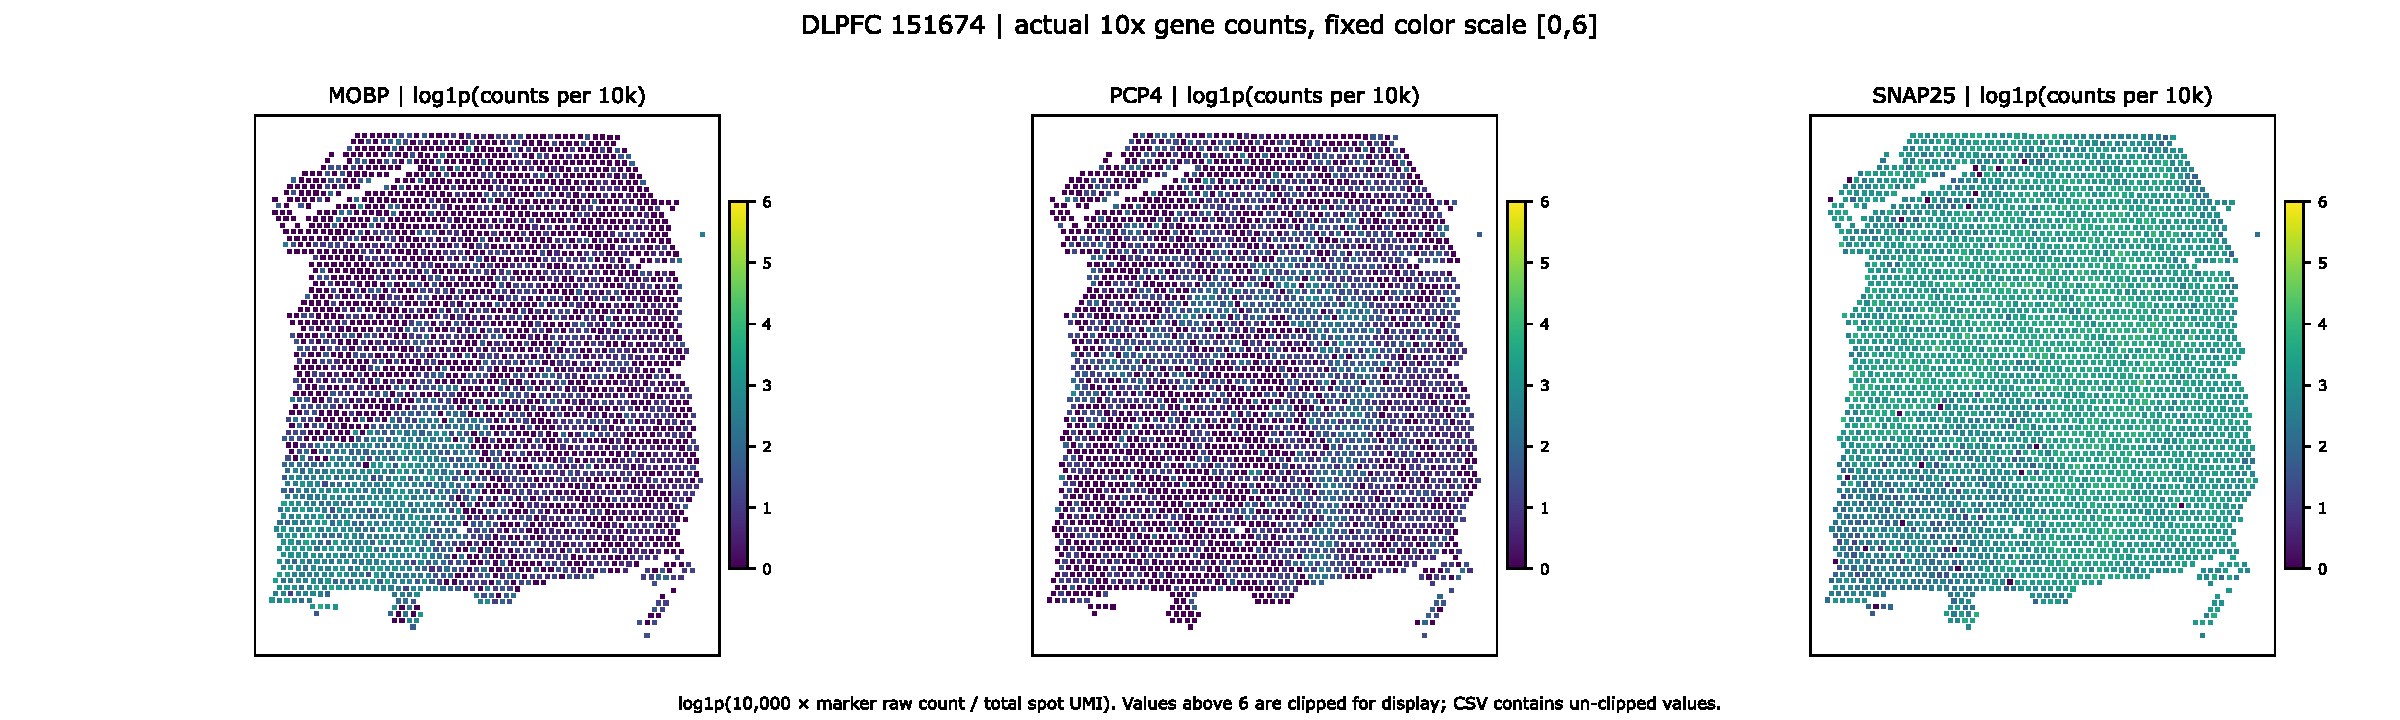
\includegraphics[width=0.97\linewidth,height=0.72\textheight,keepaspectratio]{E4_SOURCE_FIGURES_20261122_RELEASE/figures_pdf/151674/151674_MOBP_PCP4_SNAP25_expression.pdf}
\captionof{figure}{DLPFC切片151674：MOBP/PCP4/SNAP25表达三联图（原始E4图件转换的矢量PDF；聚类编号未根据参考标签重排）。}
\label{fig:cc-e4-app-151674-markers}
\end{minipage}\par\medskip
}{%
\par\noindent\emph{[编译提示：未找到该图件的PDF，请检查相对路径。]}\par
}
\IfFileExists{E4_SOURCE_FIGURES_20261122_RELEASE/figures_pdf/151674/151674_reference_A_B_confusion.pdf}{%
\par\noindent\begin{minipage}{\linewidth}
\centering
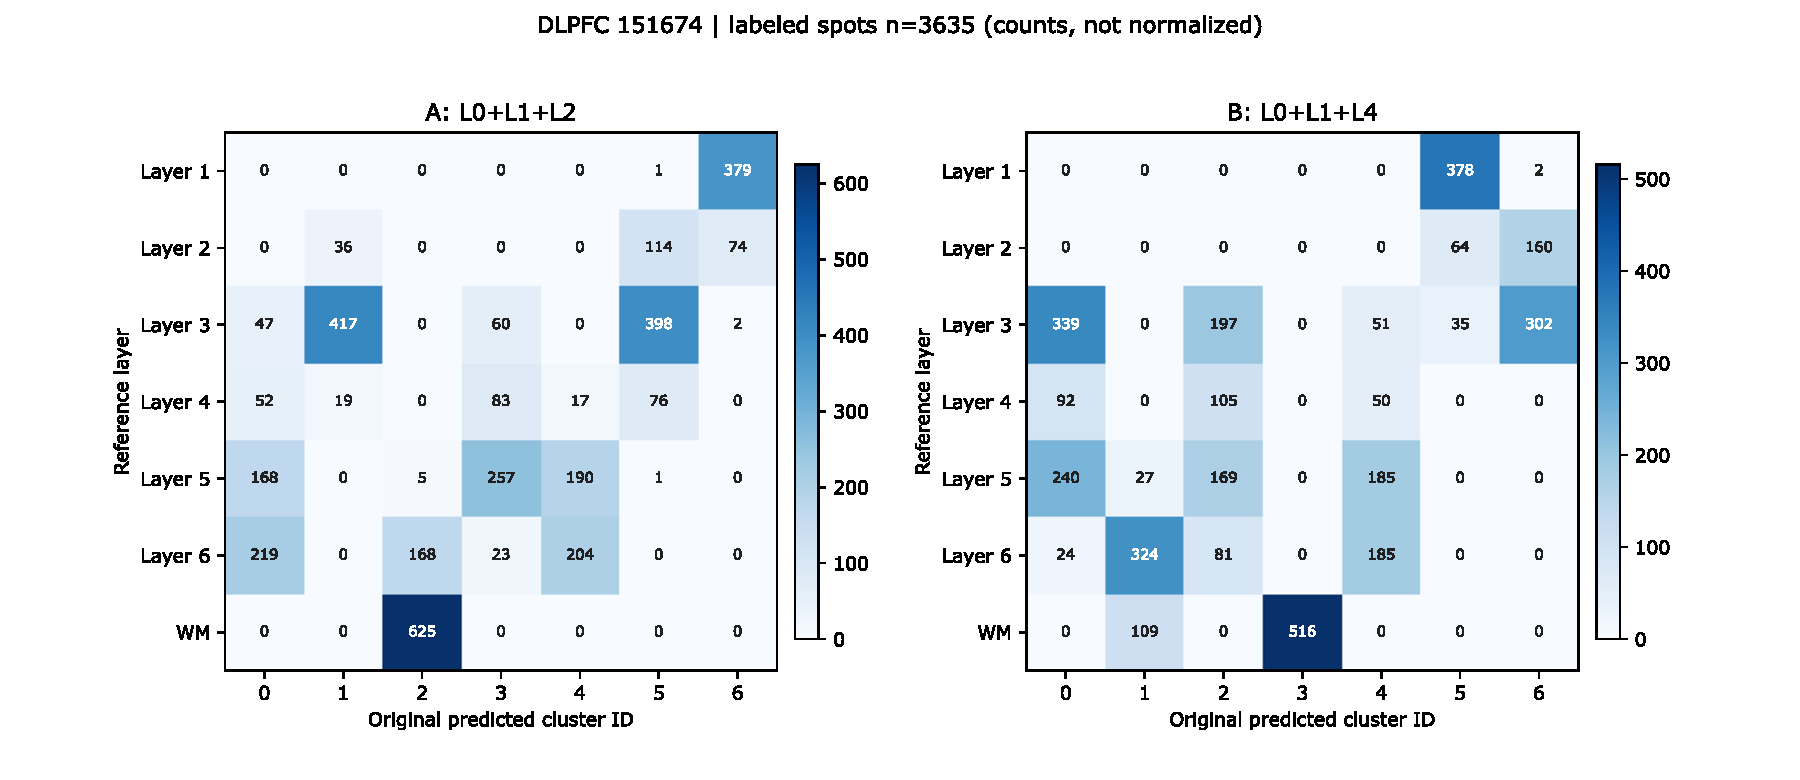
\includegraphics[width=0.97\linewidth,height=0.72\textheight,keepaspectratio]{E4_SOURCE_FIGURES_20261122_RELEASE/figures_pdf/151674/151674_reference_A_B_confusion.pdf}
\captionof{figure}{DLPFC切片151674：参考层与A/B簇交叉计数图（原始E4图件转换的矢量PDF；聚类编号未根据参考标签重排）。}
\label{fig:cc-e4-app-151674-confusion}
\end{minipage}\par\medskip
}{%
\par\noindent\emph{[编译提示：未找到该图件的PDF，请检查相对路径。]}\par
}
\subsection{DLPFC切片151675}
\IfFileExists{E4_SOURCE_FIGURES_20261122_RELEASE/figures_pdf/151675/151675_reference_A_B_spatial.pdf}{%
\par\noindent\begin{minipage}{\linewidth}
\centering
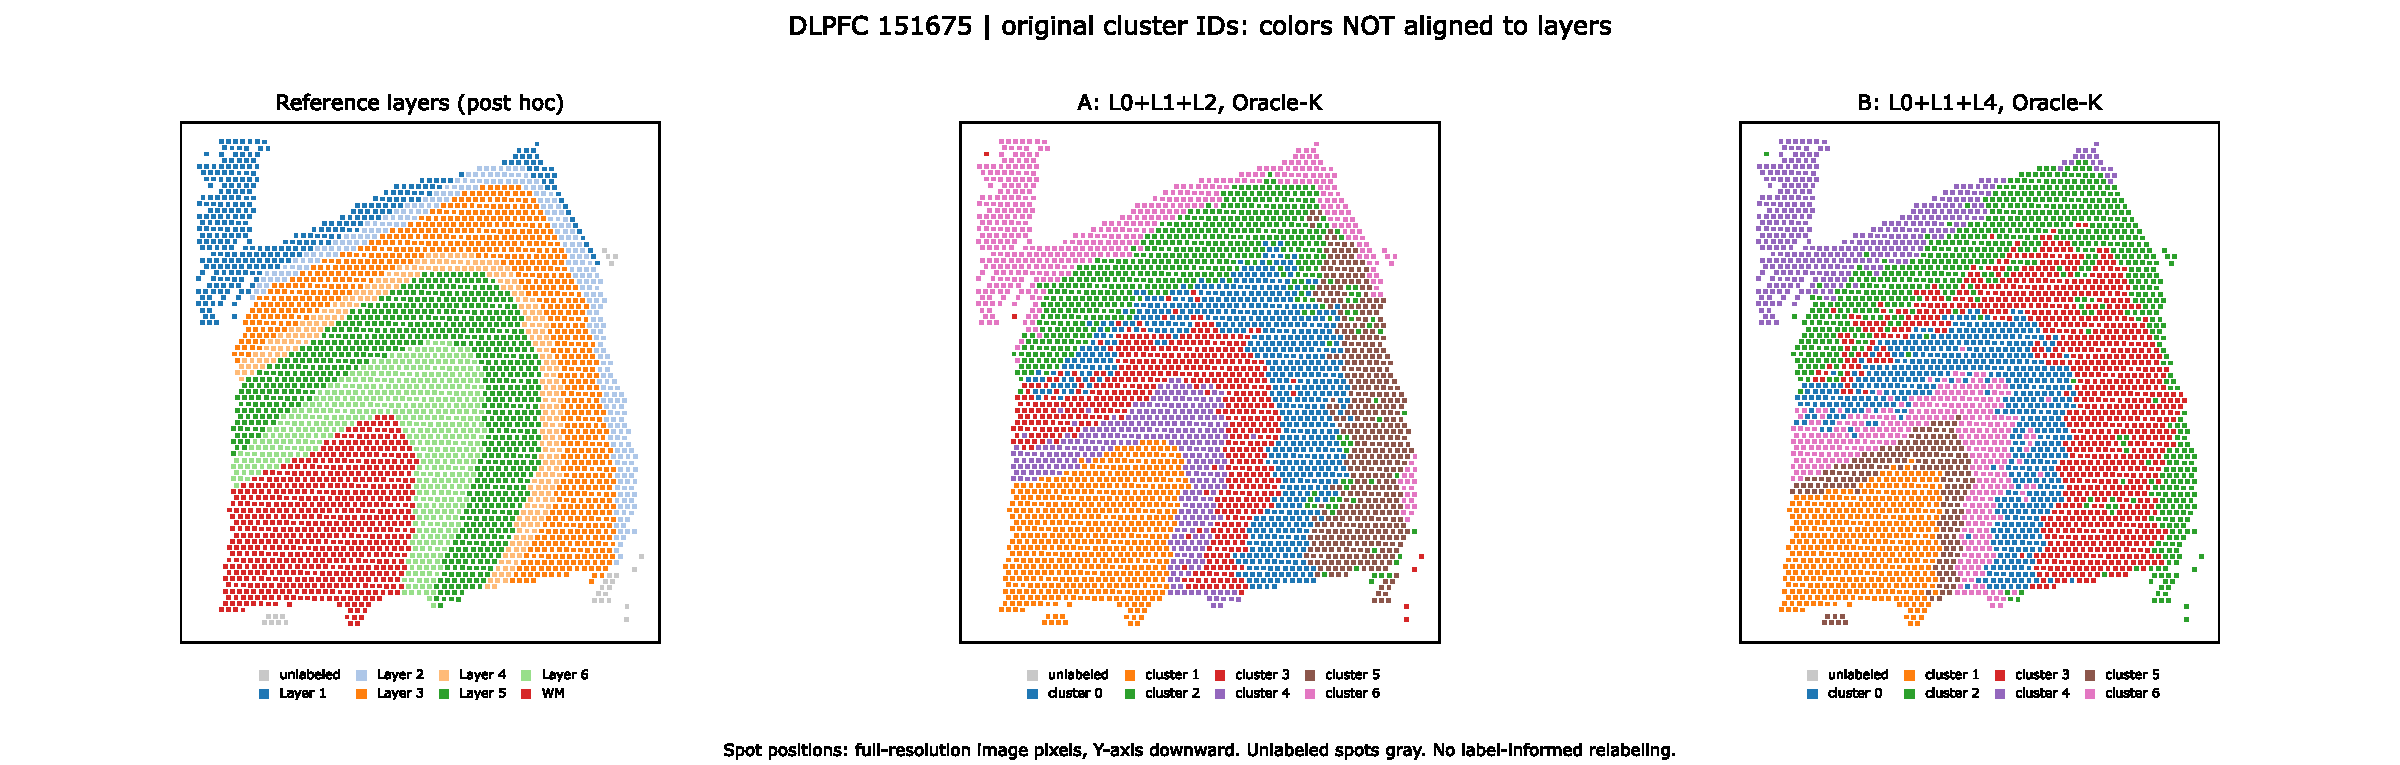
\includegraphics[width=0.97\linewidth,height=0.72\textheight,keepaspectratio]{E4_SOURCE_FIGURES_20261122_RELEASE/figures_pdf/151675/151675_reference_A_B_spatial.pdf}
\captionof{figure}{DLPFC切片151675：参考层与A/B原始聚类三联图（原始E4图件转换的矢量PDF；聚类编号未根据参考标签重排）。}
\label{fig:cc-e4-app-151675-map}
\end{minipage}\par\medskip
}{%
\par\noindent\emph{[编译提示：未找到该图件的PDF，请检查相对路径。]}\par
}
\IfFileExists{E4_SOURCE_FIGURES_20261122_RELEASE/figures_pdf/151675/151675_MOBP_PCP4_SNAP25_expression.pdf}{%
\par\noindent\begin{minipage}{\linewidth}
\centering
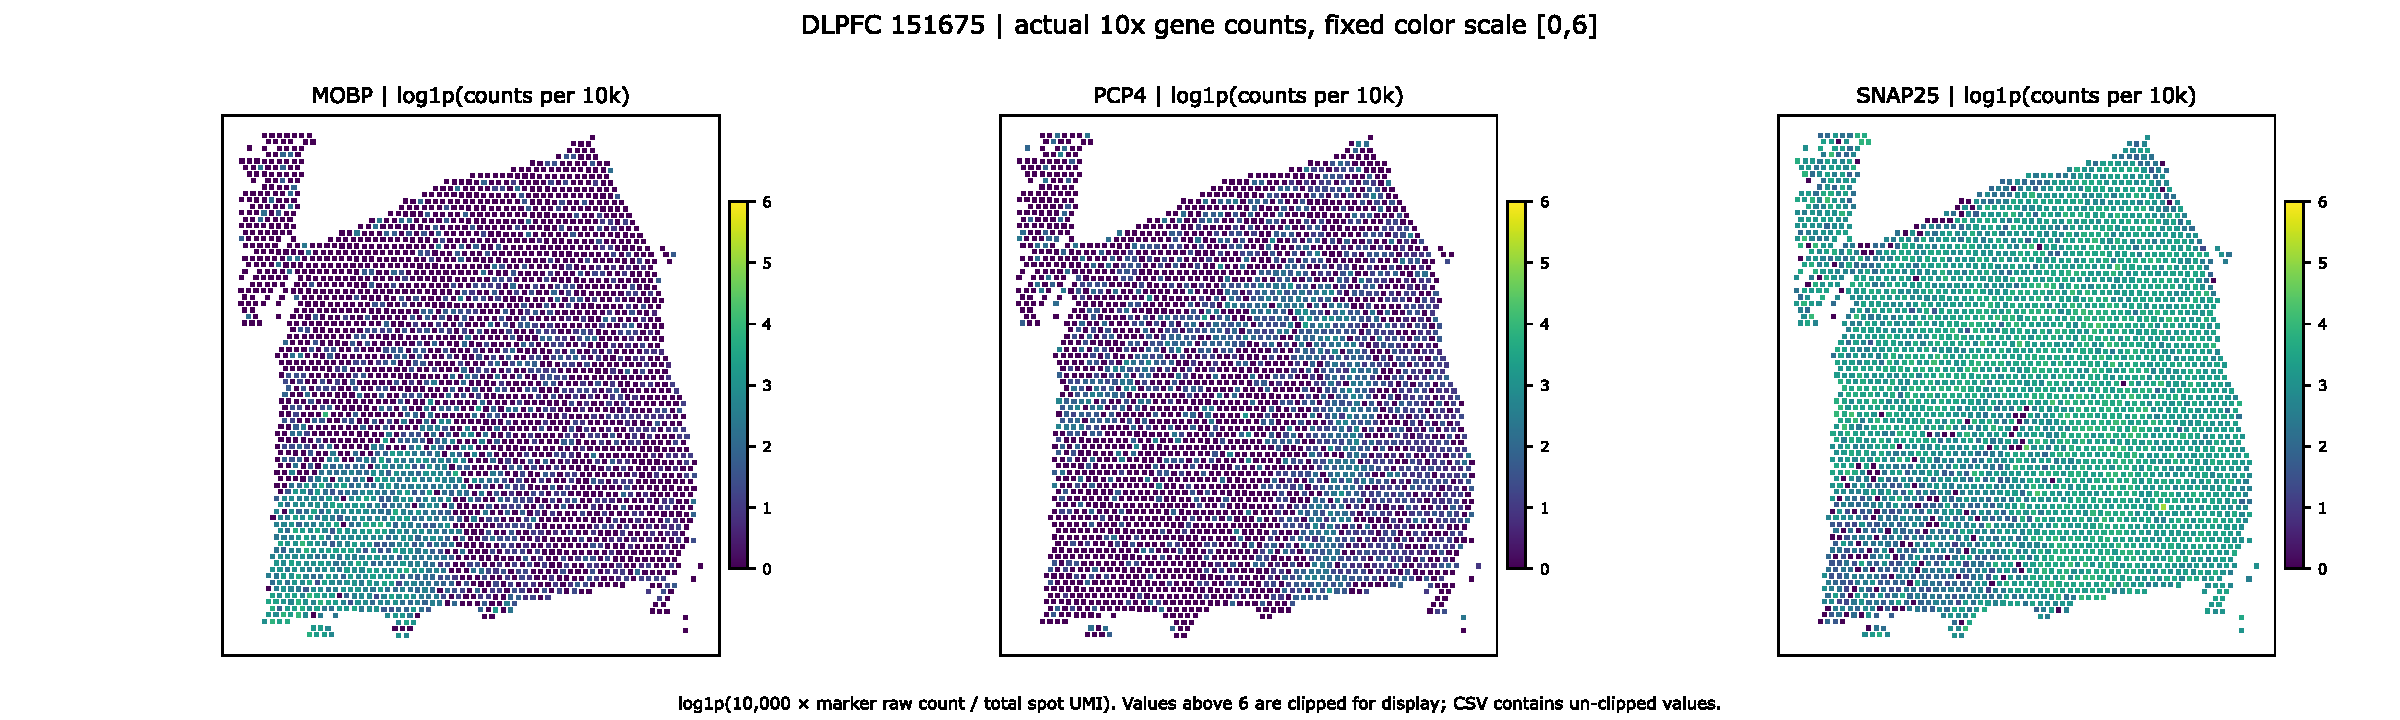
\includegraphics[width=0.97\linewidth,height=0.72\textheight,keepaspectratio]{E4_SOURCE_FIGURES_20261122_RELEASE/figures_pdf/151675/151675_MOBP_PCP4_SNAP25_expression.pdf}
\captionof{figure}{DLPFC切片151675：MOBP/PCP4/SNAP25表达三联图（原始E4图件转换的矢量PDF；聚类编号未根据参考标签重排）。}
\label{fig:cc-e4-app-151675-markers}
\end{minipage}\par\medskip
}{%
\par\noindent\emph{[编译提示：未找到该图件的PDF，请检查相对路径。]}\par
}
\IfFileExists{E4_SOURCE_FIGURES_20261122_RELEASE/figures_pdf/151675/151675_reference_A_B_confusion.pdf}{%
\par\noindent\begin{minipage}{\linewidth}
\centering
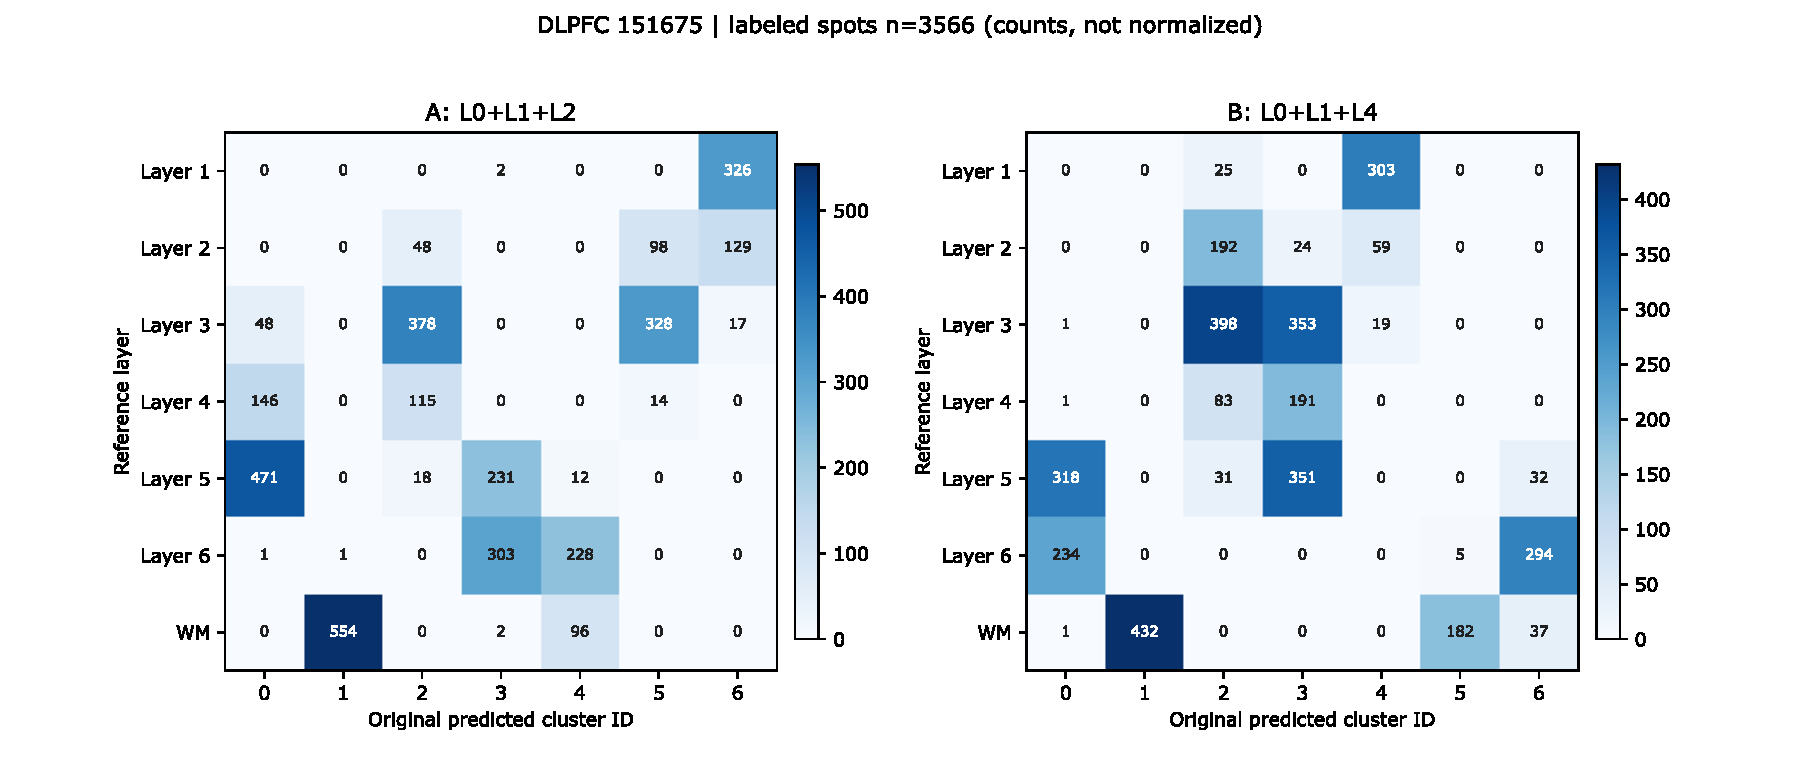
\includegraphics[width=0.97\linewidth,height=0.72\textheight,keepaspectratio]{E4_SOURCE_FIGURES_20261122_RELEASE/figures_pdf/151675/151675_reference_A_B_confusion.pdf}
\captionof{figure}{DLPFC切片151675：参考层与A/B簇交叉计数图（原始E4图件转换的矢量PDF；聚类编号未根据参考标签重排）。}
\label{fig:cc-e4-app-151675-confusion}
\end{minipage}\par\medskip
}{%
\par\noindent\emph{[编译提示：未找到该图件的PDF，请检查相对路径。]}\par
}
\subsection{DLPFC切片151676}
\IfFileExists{E4_SOURCE_FIGURES_20261122_RELEASE/figures_pdf/151676/151676_reference_A_B_spatial.pdf}{%
\par\noindent\begin{minipage}{\linewidth}
\centering
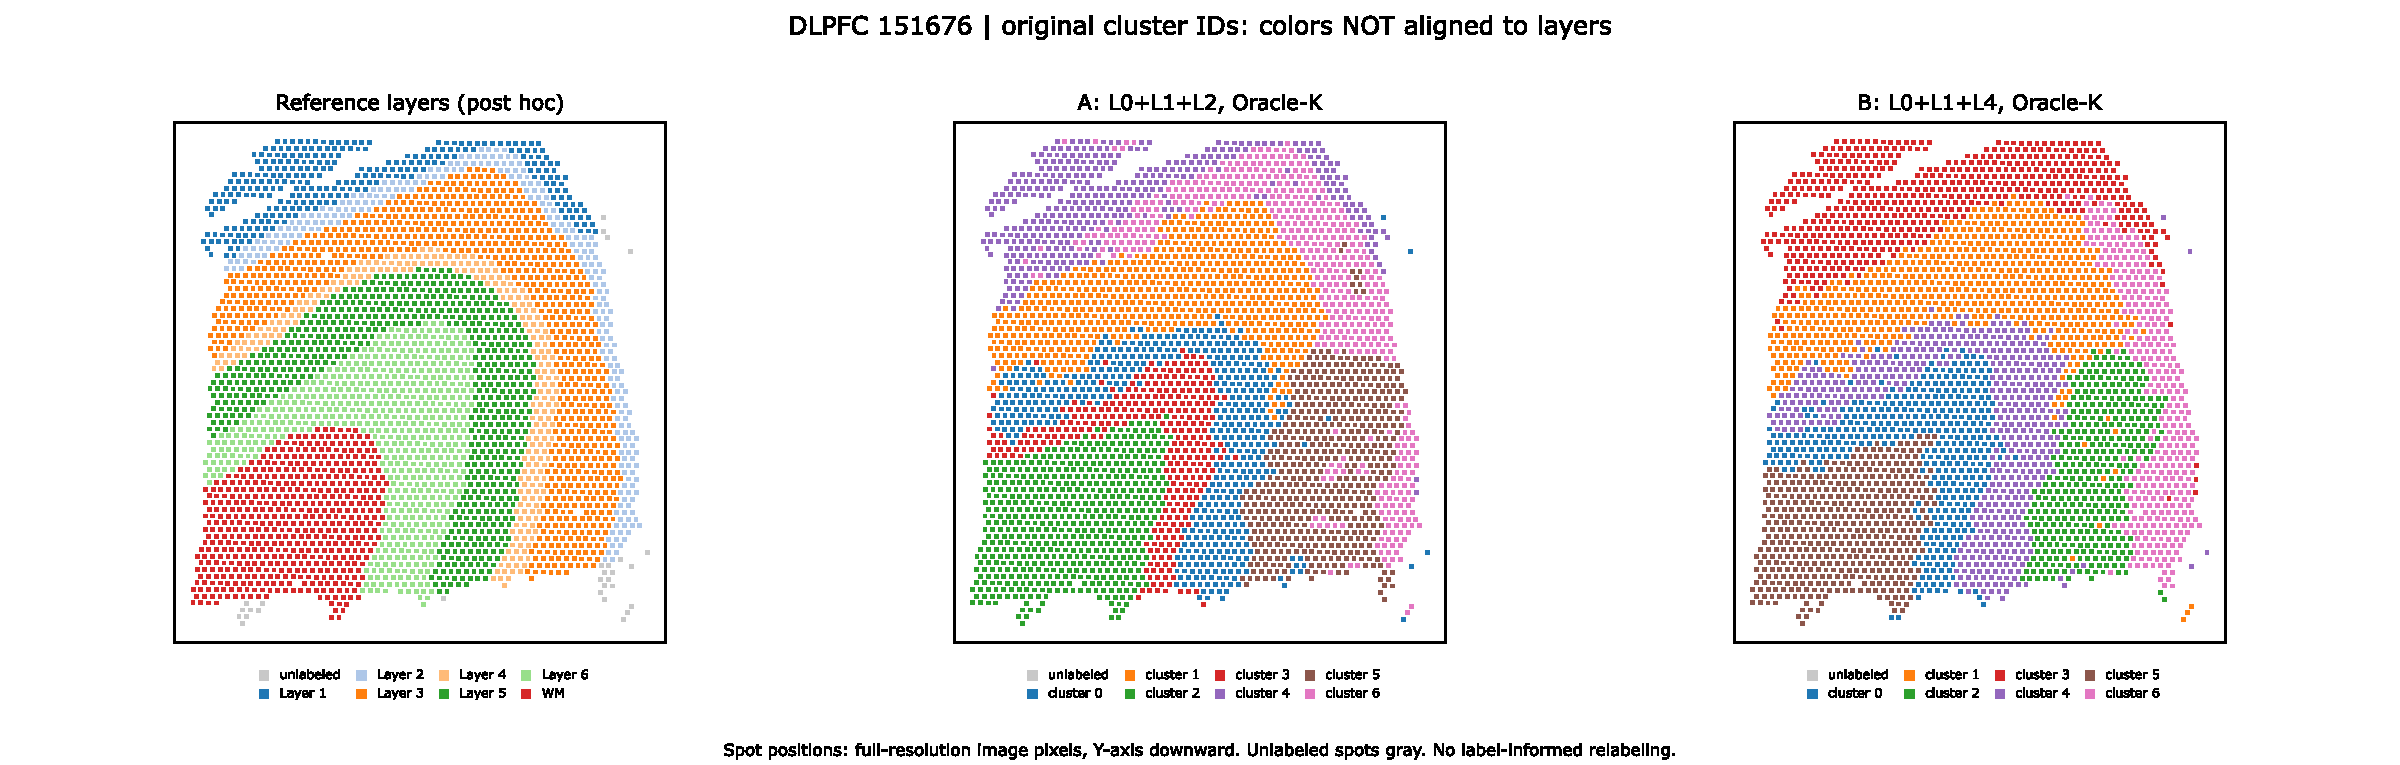
\includegraphics[width=0.97\linewidth,height=0.72\textheight,keepaspectratio]{E4_SOURCE_FIGURES_20261122_RELEASE/figures_pdf/151676/151676_reference_A_B_spatial.pdf}
\captionof{figure}{DLPFC切片151676：参考层与A/B原始聚类三联图（原始E4图件转换的矢量PDF；聚类编号未根据参考标签重排）。}
\label{fig:cc-e4-app-151676-map}
\end{minipage}\par\medskip
}{%
\par\noindent\emph{[编译提示：未找到该图件的PDF，请检查相对路径。]}\par
}
\IfFileExists{E4_SOURCE_FIGURES_20261122_RELEASE/figures_pdf/151676/151676_MOBP_PCP4_SNAP25_expression.pdf}{%
\par\noindent\begin{minipage}{\linewidth}
\centering
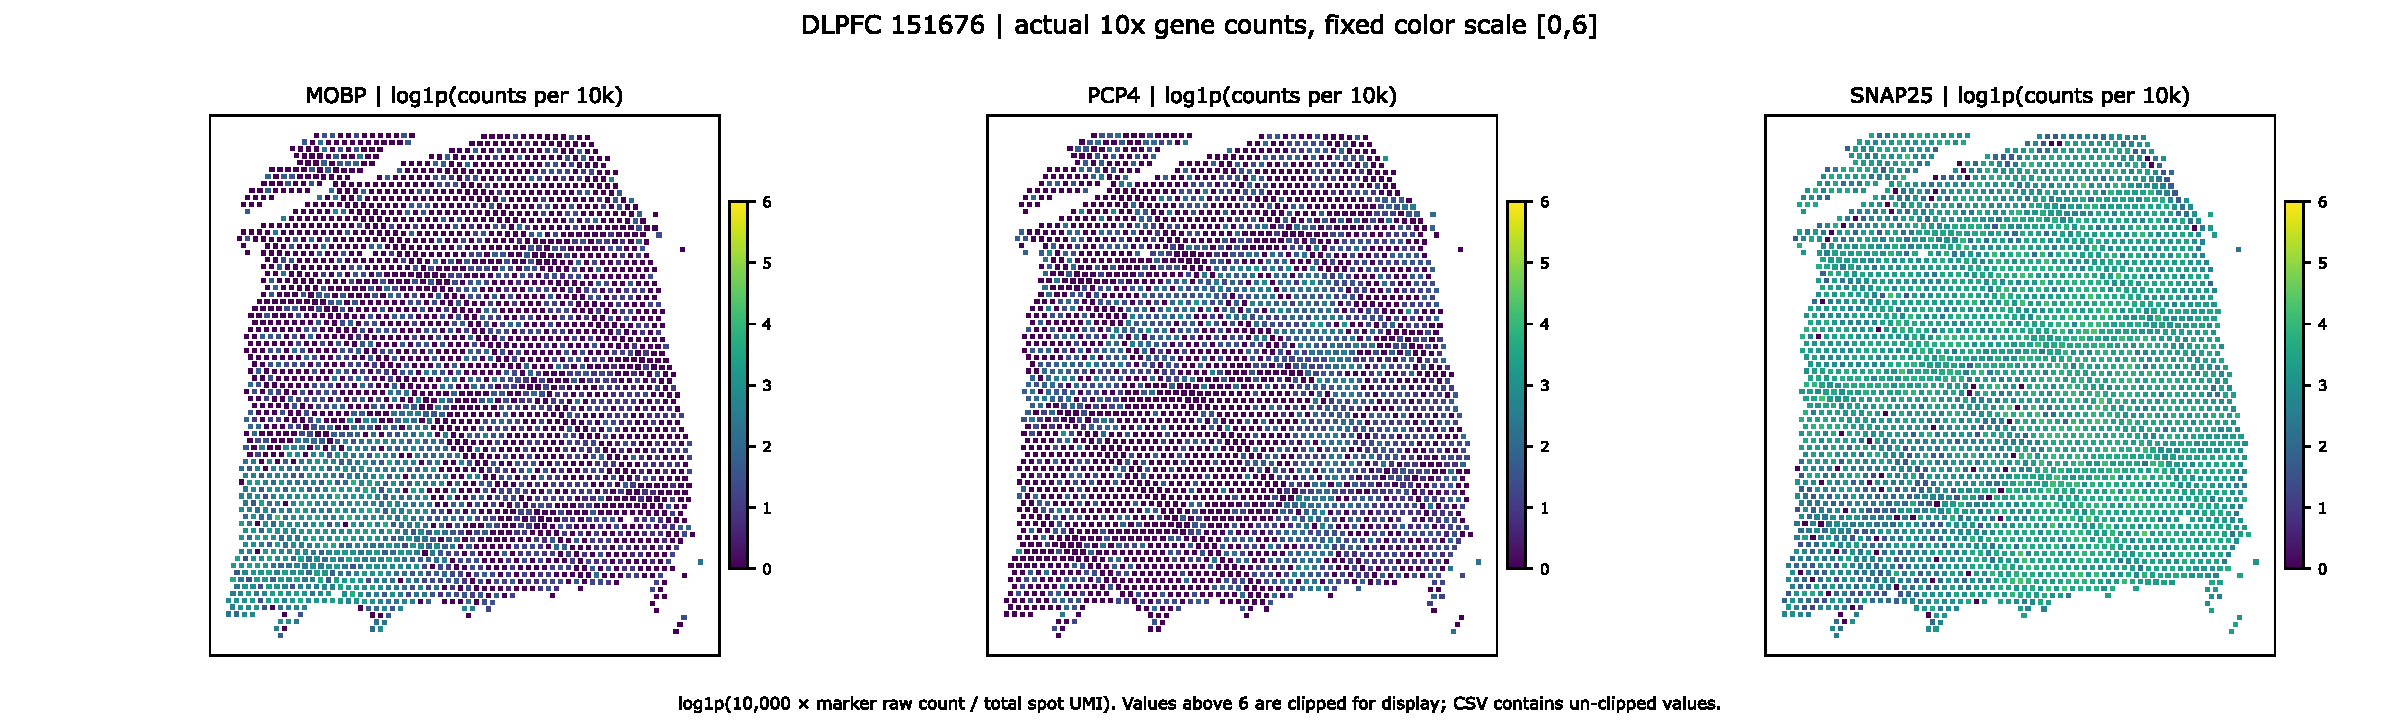
\includegraphics[width=0.97\linewidth,height=0.72\textheight,keepaspectratio]{E4_SOURCE_FIGURES_20261122_RELEASE/figures_pdf/151676/151676_MOBP_PCP4_SNAP25_expression.pdf}
\captionof{figure}{DLPFC切片151676：MOBP/PCP4/SNAP25表达三联图（原始E4图件转换的矢量PDF；聚类编号未根据参考标签重排）。}
\label{fig:cc-e4-app-151676-markers}
\end{minipage}\par\medskip
}{%
\par\noindent\emph{[编译提示：未找到该图件的PDF，请检查相对路径。]}\par
}
\IfFileExists{E4_SOURCE_FIGURES_20261122_RELEASE/figures_pdf/151676/151676_reference_A_B_confusion.pdf}{%
\par\noindent\begin{minipage}{\linewidth}
\centering
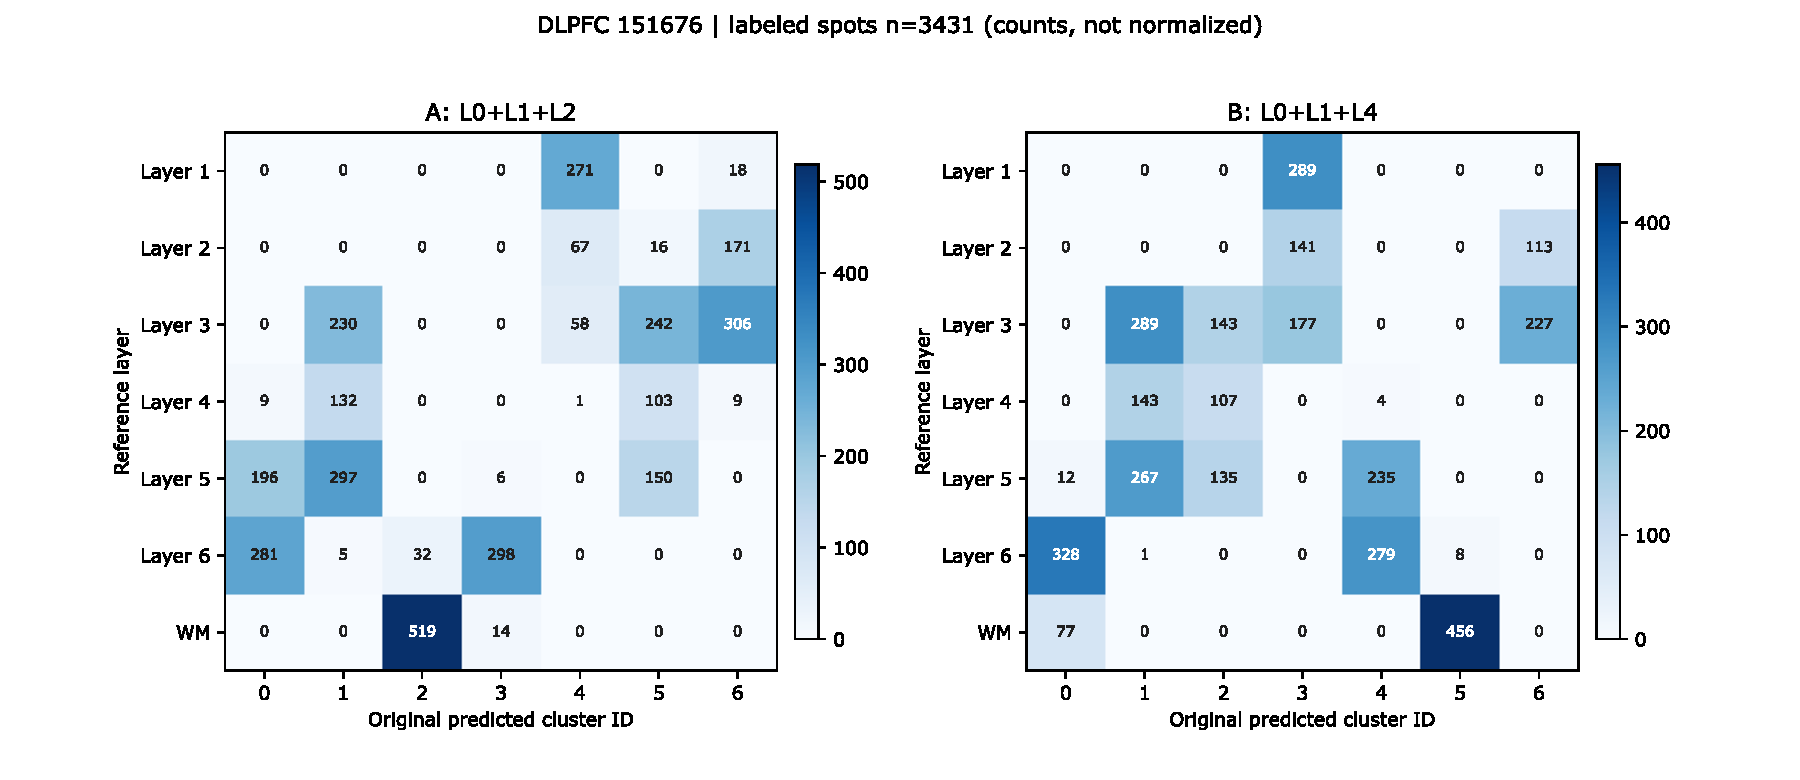
\includegraphics[width=0.97\linewidth,height=0.72\textheight,keepaspectratio]{E4_SOURCE_FIGURES_20261122_RELEASE/figures_pdf/151676/151676_reference_A_B_confusion.pdf}
\captionof{figure}{DLPFC切片151676：参考层与A/B簇交叉计数图（原始E4图件转换的矢量PDF；聚类编号未根据参考标签重排）。}
\label{fig:cc-e4-app-151676-confusion}
\end{minipage}\par\medskip
}{%
\par\noindent\emph{[编译提示：未找到该图件的PDF，请检查相对路径。]}\par
}

\clearpage
}{\PackageError{CellCharterPreview}{Required E4 figure PDF missing; 36-figure appendix cannot be omitted}{Compile in the complete project repository with figures_pdf present; do not mistake a shortened PDF for a complete thesis preview.}}
% P1 学术写作版（2026-11-24）：数据、代码与实验记录附录。
% 承接从正文移出的实验编号、结果文件与可复现性信息。未编译。
\section{数据、代码与实验记录}
\label{sec:cc-records-p1}

\subsection{数据可用性}
DLPFC Visium数据及人工层注释来自Maynard等公开的数据资源\cite{maynard2021}。乳腺癌Visium数据及病理区域注释来自Wu等的公开数据\cite{wu2021,wu2021zenodo}。CellCharter原作者的基准代码与结果文件取自其公开仓库\cite{cellcharteranalyses2024}；本研究用于对照的文件固定在提交\texttt{fd63ac5}，按MIT许可随本研究的记录一并保存。原始10x表达矩阵、scVI模型权重以及部分对照方法的逐spot预测，因体积较大没有放入公开仓库；正文所有表格中的数值都可以由已公开的结果文件复算。

\subsection{实验记录编号对照}
正文按研究问题组织，研究过程中的实验记录则按内部编号归档。两者的对应关系见表\ref{tab:cc-record-map-p1}。各项分析的方案文件均在相应模型拟合之前固定；每项结果都保存了逐任务的预测文件或指标文件及其SHA256校验值。

\begin{table}[htbp]
\centering
\caption{正文内容与实验记录编号、结果目录的对应关系（目录相对于\texttt{experiments/cellcharter\_dlpfc/}）}
\label{tab:cc-record-map-p1}
\small
\begin{tabularx}{\linewidth}{p{1.2cm}Xp{1.8cm}X}
\toprule
编号 & 内容 & 正文位置 & 结果目录\\
\midrule
E1/E2 & 10种邻域配置$\times$10个GMM种子，参考类别数 & 第\ref{subsec:cc-res-neighborhood-p1}节 & \texttt{E1E2\_20261119\_RELEASE}；逐任务预测见\texttt{E3B\_E1E2\_1200\_PREDICTIONS\_20261122}\\
E3c & 固定$K=5$--9网格 & 第\ref{subsec:cc-res-k-p1}节 & \texttt{E3C\_20261120\_RELEASE}\\
E3d & 逐切片稳定性选K及事后评分 & 第\ref{subsec:cc-res-k-p1}节 & \texttt{E3D\_20261122\_RELEASE}，\texttt{E3D\_POSTHOC\_20261122\_RELEASE}\\
E3b & 严格与容差边界评价（事后） & 第\ref{subsec:cc-res-boundary-p1}节 & \texttt{E3B\_E1E2\_1200\_POSTHOC\_20261122\_RELEASE}，\texttt{E3B\_E3D48\_POSTHOC\_20261122\_RELEASE}\\
E4 & 空间分布、标记基因与交叉计数图 & 第\ref{subsec:cc-res-maps-p1}节及附录 & \texttt{E4\_SOURCE\_FIGURES\_20261122\_RELEASE}\\
E5a & DLPFC成熟方法对照 & 第\ref{subsec:cc-res-baselines-p1}节 & \texttt{E5A\_20261122\_RELEASE}\\
E5b & 乳腺癌患者队列 & 第\ref{subsec:cc-res-external-p1}节 & \texttt{E5B\_20261122\_RELEASE}\\
汇总 & 描述性再汇总表T1--T11（只读、可复算） & 各节表注 & \texttt{REV\_P0\_20261124/derived}，\texttt{P1\_20261124/derived}\\
\bottomrule
\end{tabularx}
\end{table}

\subsection{可复现性说明}
各分析的方案文件包括：邻域表征比较的GMM方案（\texttt{THIRD\_PAPER\_E1E2\_FROZEN\_GMM\_PROTOCOL\_20261113.md}）、固定K网格方案（\texttt{THIRD\_PAPER\_E3C\_K\_SENSITIVITY\_FROZEN\_PROTOCOL\_20261119.md}）、稳定性选K方案（\texttt{E3D\_AUTOK\_FROZEN\_PROTOCOL\_20261120.md}）、成熟方法对照方案（\texttt{E5A\_FROZEN\_FAIR\_BASELINE\_PROTOCOL\_20261120.md}）和外部队列方案（\texttt{E5B\_FROZEN\_EXTERNAL\_VALIDATION\_PROTOCOL\_20261121.md}）。正文中的描述性再汇总，由\texttt{REV\_P0\_20261124/rev\_p0\_derived\_summaries\_v1.py}和\texttt{P1\_20261124/p1\_additional\_summaries\_v1.py}从上述结果文件只读计算，只依赖Python标准库；输入与输出的SHA256分别记录在两处\texttt{derived/MANIFEST\_SHA256.csv}中。DLPFC特征生成脚本为\texttt{scripts/cellcharter/prepare\_dlpfc\_10\_features.py}，所用的软件版本记录在各特征缓存的配置文件中。


\clearpage
\bibliographystyle{unsrt}
\bibliography{thesis_cellcharter_references_p1_20261124}
\end{document}
